\documentclass[english,12pt,jmp,graphicx]{revtex4-1}
%\documentclass[jmp,graphicx]{revtex4-1}
%\documentclass[aip,reprint]{revtex4-1}

\usepackage{graphicx}% Include figure files
\usepackage{dcolumn}% Align table columns on decimal point
\usepackage{bm}% bold math
\usepackage{amsmath,amssymb,latexsym,mathrsfs}

\draft % marks overfull lines with a black rule on the right

\newtheorem{lemma}{Lemma}[section]
\newtheorem{theorem}{Theorem}[section]
\newtheorem{proof}{Proof}[section]
\newtheorem{definition}{Definition}[section]
\newtheorem{remark}{Remark}[section]
\newtheorem{corollary}{Corollary}[section]


\newcommand{\ph}{\hat{\phi}}
\newcommand{\pt}{\tilde{\phi}}
\newcommand{\pc}{\check{\phi}}
\newcommand{\gh}{\hat{\gamma}}
\newcommand{\Dh}{\hat{\Delta}}
\newcommand{\dha}{\hat{\delta}}
\newcommand{\qh}{\hat{q}}
\newcommand{\xh}{\hat{x}}
\newcommand{\HM}{\mathcal{H}_{\text{max}}}
\newcommand{\Hm}{\mathcal{H}_{\text{min}}}
\newcommand{\sech}{\rm \hspace{0.7mm}sech}
\newcommand{\I}{\mathrm{i}}
\newcommand{\hh}{\hat{h}}
\newcommand{\mh}{m_r}
\newcommand{\mt}{m_i}

\begin{document}

% Use the \preprint command to place your local institutional report number 
% on the title page in preprint mode.
% Multiple \preprint commands are allowed.
%\preprint{}

\title{The Ising Model
and Critical Behavior of Transport \\in Binary Composite Media} %Title of paper

% repeat the \author .. \affiliation  etc. as needed
% \email, \thanks, \homepage, \altaffiliation all apply to the current author.
% Explanatory text should go in the []'s, 
% actual e-mail address or url should go in the {}'s for \email and \homepage.
% Please use the appropriate macro for the type of information

% \affiliation command applies to all authors since the last \affiliation command. 
% The \affiliation command should follow the other information.

\author{N. B. Murphy$^1$ and K. M. Golden$^1$}
%\email[]{benmurphy.math@gmail.com}
%\homepage[]{Your web page}
%\thanks{}
%\altaffiliation{}
\affiliation{University of Utah, Department of Mathematics, 155 S 1400
  E RM 233, Salt Lake City, UT 84112-0090, USA}
%
%\collaboration{K. M. Golden$^1$}
%\author{K. M. Golden$^1$}
%\email[]{benmurphy.math@gmail.com}
%\homepage[]{Your web page} 
%\thanks{}
%\altaffiliation{}
%\affiliation{University of Utah, Department of Mathematics, 155 S 1400
%  E RM 233, Salt Lake City, UT 84112-009, USA}

% Collaboration name, if desired (requires use of superscriptaddress option in \documentclass). 
% \noaffiliation is required (may also be used with the \author command).
%\collaboration{}
%\noaffiliation

\date{\today}

\begin{abstract}
%
We present a general theory for critical behavior of transport in
binary composite media. The theory holds for lattice and continuum
percolation models in both the static case with real parameters and
the quasi--static case (frequency dependent) with complex
parameters. Through a direct, analytic correspondence between the
magnetization of the Ising model and the effective parameter problem
of two phase random media, we show that the critical exponents of the
transport coefficients satisfy the standard scaling relations for
phase transitions in statistical mechanics. Our work also shows that
delta components form in the underlying spectral measures at the
spectral endpoints precisely at the percolation threshold $p_c$ and at
$1-p_c$. This is analogous to the Lee-Yang-Ruelle characterization of
the Ising model phase transition, and identifies these transport
transitions with the collapse of spectral gaps in these measures. 
%
\end{abstract}

%\pacs{}% insert suggested PACS numbers in braces on next line

\maketitle %\maketitle must follow title, authors, abstract and \pacs

% Body of paper goes here. Use proper sectioning commands. 
% References should be done using the \cite, \ref, and \label commands
%
%------------------------------------------------------------------------
\section{Introduction}\label{sec:Introduction}
%
Lattice and continuum percolation models have been used to study a
broad range of disordered composite materials including semiconductors 
\cite{Efros-84}, radar absorbing coatings \cite{Kusy:N-58},
%thin films \cite{Davis:OC-70},
bone
%\cite{Golden:JoB:337},
\cite{Sasaki:JTB:25,Golden:JoB:337},
rocks \cite{Bourbie:JGR-11524,Broadbent:PCPS-629}, 
glacial ice \cite{Enting:1985:LSM}, polycrystalline metals
\cite{Chen:PRL:2007}, carbon nanotube composites
\cite{Kyrylyuk:PNAS:2008}, and sea ice
\cite{Golden:2007:GRL,Golden:S-2238}. A key 
feature of these materials is the critical dependence of the effective
transport properties on the connectedness, or percolation
characteristics, of a particular component. The behavior of such
composite media is particularly challenging to describe physically,
and to predict mathematically.  

Here we construct a mathematical framework which unifies the critical
theory of transport in two phase random media. By adapting techniques
developed by G. A. Baker for the Ising model \cite{Baker-1990}, we
provide a detailed description of percolation--driven critical
transitions in transport exhibited by such media. The most natural
formulation is in terms of the conduction problem in the continuum
$\mathbb{R}^d$, which includes the lattice $\mathbb{Z}^d$ as a special
case \cite{Golden:JMP-5627,Golden:CMP-473}. Although, symmetries
in Maxwell's equations \cite{MILTON:2002:TC} immediately extend our
results to the effective parameter problem of electrical
permittivity.

An original motivation for this work was to gain a better
understanding of critical transitions in the transport properties of
sea ice. In particular, fluid flow through sea ice mediates a broad
range of processes that are important to studying its role in the
climate system, and the impact of climate change on polar ecosystems
\cite{Golden:NAMS:2009}. In fact, the brine microstructure of sea ice
undergoes a percolation threshold at a critical brine volume fraction
$\phi$ of about 5\% in columnar sea ice
\cite{Golden:S-2238,Golden:2007:GRL,Pringle:JGR:2009}. 
This leads to critical behavior of fluid flow, where sea ice is effectively
impermeable to fluid transport for $\phi$
below 5\%, and is increasingly permeable for $\phi$ above 5\%, which is
known as the {\it rule of fives} \cite{Golden:S-2238}.
Percolation theory can then be used to capture the behavior of
the fluid permeability of sea ice \cite{Golden:2007:GRL}.
There has also been evidence \cite{Gully:PhysB:357,Orum:PRSLA:2011}
that this critical behavior in the
microstructure also induces similar behavior in the effective electromagnetic
properties of sea ice, such as its effective complex permittivity $\epsilon^*$.
In \cite{Gully:PhysB:357} and \cite{Orum:PRSLA:2011}, for example,
microstructural properties of the brine phase were recovered from
measurements of the complex permittivity of sea ice.
The current paper helps lay the groundwork for the analysis of
sea ice permittivity data collected in the polar regions, and how it can
be used to monitor changes in the microstructure, the fluid transport properties,
and the geophysical and biological processes that are controlled by
fluid flow.



%------------------------------------------------------------------------
\section{Background and Summary of the Results}\label{sec:Background}
%
The partition function $Z$ of the Ising model is a polynomial
in the activity variable \cite{Lee:PR:411,Baker-1990,Ruelle-1969,Ruelle:AM:589}.
In 1952 Lee and Yang \cite{Lee:PR:411} showed that the 
roots of $Z$ lie on the unit circle, which is
known as the Lee--Yang Theorem \cite{Lee:PR:411,Ruelle-1969}.
They also demonstrated that 
the distribution of the roots determines 
the associated equation of state
\cite{Yang:PR:404}, and that the properties of 
the system, in relation to phase transitions, are governed by the
behavior of these roots near the positive real axis.   

In 1968 Baker \cite{Baker:PRL-990} used the Lee--Yang Theorem to represent the Gibbs
free energy per spin $f=-(N\beta)^{-1}\ln{Z}$ as a logarithmic potential
\cite{Saff_Totik:97}, where $N$ is the number of spins, $\beta=(kT)^{-1}$,
$k$ is Boltzmann's constant, and $T$ is the absolute temperature.
He used this special analytic structure to prove
that the magnetization per spin $M(T,H)=-\partial f/\partial H$
\cite{Robertson-1993} may be represented in terms of a Stieltjes
function $G$ in the variable $\tau=\tanh{\beta mH}$,          
%
\begin{align}\label{Ising_Stieltjes_Fun}
  \frac{M}{m} =\tau(1+(1-\tau^2)G(\tau^2)), \quad
  G(\tau^2)=\int_0^\infty\frac{d\psi(y)}{1+\tau^2y}\,, % for single column paper
  %\frac{M(T,H)}{m} =\tau(1+(1-\tau^2)G(\tau^2)), \\
  %G(\tau^2)=\int_0^\infty\frac{d\psi(y)}{1+\tau^2y}\;,\notag % for two column paper
\end{align}
%
where $H$ is the applied magnetic field strength, $m$ is the
(constant) magnetic dipole moment of each spin \cite{Griffiths-1999},
and $\psi$ is a non--negative definite measure
\cite{Baker:PRL-990,Baker-1990}. The integral representation in
\eqref{Ising_Stieltjes_Fun} immediately leads to the inequalities    
%
\begin{align}\label{eq:Gtau_inneq}
  G\geq0, \qquad \frac{\partial G}{\partial u}\leq0, \qquad \frac{\partial^2G}{\partial u^2}\geq0,
\end{align}
%
where $u=\tau^2$. The last formula in equation \eqref{eq:Gtau_inneq} is
the GHS inequality, which is an important tool in the study of the
Ising model \cite{Golden:JMP-5627}. 

In 1970 Ruelle  \cite{Ruelle:PRL:303} extended the Lee--Yang Theorem and proved that
there exists a \emph{gap} $\theta_0(T)>0$ in the roots of $Z$ about the positive
real axis for high temperatures. Moreover, he
proved that the gap collapses, $\theta_0(T)\to0$, as $T$ decreases to a
critical temperature $T_c>0$. Consequently, the temperature--driven
phase transition (spontaneous magnetization) is unique, and is
characterized by the pinching of the real axis by the roots of $Z$
\cite{Ruelle-1969}.   

Baker \cite{Baker:PRB:1184,Baker-1990} then exploited the
Lee--Yang--Ruelle Theorem to provide a detailed description of the 
critical behavior of the parameters characterizing 
the phase transition exhibited by the Ising model
\cite{Christensen-2005}. He defined a critical 
exponent $\Delta$ for the gap in the distribution of the Lee--Yang--Ruelle
zeros, $\theta_0(T)\sim(T-T_c)^\Delta$, as $T\to T_c^+$, and proved that
%the support $\Sigma_\psi$ of
the measure $\psi$ is supported on the compact interval
$[0,S(T)]$ for $T>T_c\,$, with $S(T)\sim(T-T_c)^{-2\Delta}$ as
$T\to T_c^+$. He demonstrated that the moments $\psi_n=\int_0^\infty y^n\,d\psi(y)$ of $\psi$
diverge as $T\to T_c^+$ according to the power law $\psi_n\sim(T-T_c)^{-\gamma_n}$,
$n\geq0$, by proving that the sequence $\gamma_n$ satisfies Baker's
inequalities $\gamma_{n+1}-2\gamma_n+\gamma_{n-1}\geq0$. They imply that this sequence
increases at least linearly with $n$. He later proved that this
sequence is actually linear in $n$, $\gamma_n=\gamma+2\Delta n$, with constant gap
$\gamma_i-\gamma_{i-1}=2\Delta$ \cite{Baker-1990}. The critical exponent $\gamma$ is
defined via the magnetic susceptibility per spin $\chi=\partial M/\partial H=-\partial^2f/\partial
H^2\sim(T-T_c)^{-\gamma}$, as $T\to T_c^+$. 

The phase transition may be concisely described with two
other critical exponents. When $H=0$, $M(T,0)\sim(T-T_c)^\beta$, as $T\to T_c^-$,
where the critical exponent $\beta$ is not to be confused with
$(kT)^{-1}$, and along the critical isotherm $T=T_c$, $M(T_c,H)\sim H^{1/\delta}$,
as $H\to0$ \cite{Christensen-2005,Baker-1990}. Using the integral
representation in \eqref{Ising_Stieltjes_Fun}, Baker obtained 
(two--parameter) scaling relations for these critical exponents
\cite{Baker-1990} 
%
\begin{align}\label{eq:Ising_Scaling_Relations}
  \beta=\Delta-\gamma, \qquad \delta=\Delta/(\Delta-\gamma), \qquad \gamma_n=\gamma+2\Delta n.
\end{align}
%
The critical exponent $\gamma$, for example, is defined
in terms of the following limit, and $\gamma$ exists when this limit exists
\cite{Baker-1990},
% 
\begin{align}\label{eq:Critical_Exponent_Existence}
  \gamma=\limsup_{T\to T_c^+, \;H=0}\left(\frac{-\ln \chi(T,H)}{\ln(T-T_c)}  \right).
\end{align}
%

In 1997 Golden \cite{Golden:PRL-3935} demonstrated that Baker's
critical theory may be adapted to provide a precise description of
percolation--driven critical transitions in transport, exhibited by
two phase random media in the static regime. This result puts these
two classes of seemingly unrelated problems on an equal mathematical
footing. He did so by considering percolation models of classical
conductive two phase composite media, where the connectedness of the
system is determined, for example, by the volume fraction $p$ of
inclusions with conductance $\sigma_2$ in an otherwise homogeneous medium
of conductivity $\sigma_1$, with $h=\sigma_1/\sigma_2\in[0,1]$. 
He demonstrated that the function $m(p,h)=\sigma^*(p,h)/\sigma_2$ plays the role
of the magnetization  $M(T,H)$, where $\sigma^*$ is the effective
conductivity of the medium
\cite{Bergman:PRC-377,Milton:APL-300,Golden:CMP-473}. Moreover, he 
showed that the volume fraction $p$ mimics the temperature $T$ while
the contrast ratio $h$ is analogous to the applied magnetic field strength $H$. 
More specifically, critical behavior of transport
arises when $h=0$ $(\sigma_1=0, \ 0<\sigma_2<\infty)$, as $p\to p_c^+$
\cite{Golden:PRL-3935}, and 
critical behavior of the magnetization in the Ising model 
arises when $H=0$, as $T\to T_c^+$
\cite{Christensen-2005}. Using these mathematical
parallels, it was shown that the critical exponents of transport 
satisfy an analogue of Baker's %two--parameter
scaling relations \eqref{eq:Ising_Scaling_Relations}.

Here, using a novel unified approach, we reproduce Golden's
static results $(h\in\mathbb{R})$ and obtain the analogous static
results associated with a conductive--superconductive medium in terms
of $w(p,z)=\sigma^*(p,z)/\sigma_1$, where $z=1/h$. Using Stieltjes function
integral representations of $m(p,h;\mu)$ and $w(p,z;\alpha)$, where $\mu$ and
$\alpha$ are each spectral measures of a random self--adjoint operator, we
determine the (two--parameter) critical exponent scaling relations of
each system. We then extend these results to the frequency dependent
quasi--static regime $(h\in\mathbb{C})$. We also link these two sets of
critical exponents.
%showing that they are all, in general, determined by only three
%critical exponents, and are determined by only two critical exponents
%under a physically consistent symmetry in the 
%properties of $\mu$ and $\alpha$.
In arbitrary finite lattice systems we
explicitly show that there are \emph{gaps} in the supports of the measures
$\alpha(d\lambda)$ and $\mu(d\lambda)$ about the spectral endpoints $\lambda=0,1$ for $p\ll1$ and
$1-p\ll1$, respectively.
%, which collapse as $p$ tends towards $p_c$.
Moreover in infinite lattice or continuum composite systems, we
demonstrate that critical transitions in transport are due to the
formation of delta
%function
components in $\mu$ and $\alpha$ located at
$\lambda=0,1$. We do so by constructing a measure $\varrho$ which is supported
on the set $\{0,1\}$ that links
%the measures
$\mu$ and $\alpha$. This general
result demonstrates that, for percolation models, the onset of
criticality (the formation of these delta components) occurs
\emph{precisely} at the percolation threshold $p_c$ and at
$1-p_c$. We stress that there are similar critical exponents involving
the effective complex permittivity $\epsilon^*$ of two phase dielectric
media \cite{Clerc:AP-191,Bergman:SSP-147}, and there are direct
analogs of our results regarding such media.     
%
%
%------------------------------------------------------------------------------
%
\section{The Analytic Continuation Method}\label{eq:TACM}
%
We now formulate the effective parameter problem for two component
conductive media. Let $(\Omega,P)$ be a probability space, and let
$\bm{\sigma}(\vec{x},\omega)$ and $\bm{\rho}(\vec{x},\omega)$ be the local 
conductivity and resistivity tensors, respectively, which are
(spatially) stationary random fields in $\vec{x}\in\mathbb{R}^d$ and
$\omega\in\Omega$. Here $\Omega$ is the set of all geometric realizations of our random
medium, $P(d\omega)$ is the underlying probability measure, which is
compatible with stationarity, and $\bm{\rho}=\bm{\sigma}^{-1}$
\cite{Golden:CMP-473}. Define the Hilbert  
space of stationary random fields $\mathscr{H}_s\subset L^2(\Omega,P)$, and the
underlying Hilbert spaces of stationary curl free
$\mathscr{H}_\times\subset\mathscr{H}_s$ and divergence free
$\mathscr{H}_{\bullet}\subset\mathscr{H}_s$ random fields   
%
\begin{align}\label{eq:curlfreeHilbert}
  &\mathscr{H}_\times=
  \{\vec{Y}(\omega)\in \mathscr{H}_s \ | \ \vec{\nabla} \times\vec{Y}=0 \text{ weakly and }
    \langle\vec{Y}\rangle=0\}, \\
&\mathscr{H}_{\bullet}=
\{\vec{Y}(\omega)\in \mathscr{H}_s \ | \ \vec{\nabla}\cdot\vec{Y}=0 \text{ weakly and }
    \langle\vec{Y}\rangle=0\},\notag
\end{align}
%
where $\vec{Y}:\Omega\mapsto\mathbb{R}^d$ and $\langle\cdot\rangle$ means ensemble average over
$\Omega$, or by an ergodic theorem spatial average over all of
${\mathbb{R}}^d$ \cite{Golden:CMP-473}.  

Consider the following variational problems: 
find $\vec{E}_f\in\mathscr{H}_\times$ and  $\vec{J}_f\in \mathscr{H}_{\bullet}$ such
that \cite{Golden:CMP-473}   
%
\begin{align}
  \label{eq:Weak_Curl_Free_Variational_Form}
 &\langle\bm{\sigma}(\vec{E}_0+\vec{E}_f)\cdot\vec{Y}\rangle=0 \quad  \forall \
  \vec{Y}\in\mathscr{H}_\times &&\text{and}
%
 &&\langle\bm{\rho}(\vec{J}_0+\vec{J}_f)\cdot\vec{Y}\rangle=0 \quad  \forall \
  \vec{Y}\in\mathscr{H}_{\bullet}\,,  
\end{align}
%
respectively.
%Under the assumption that the
When the bilinear forms
$a(\vec{u},\vec{v})=\vec{u}^{\,T}\bm{\sigma}\,\vec{v}$ and
$\tilde{a}(\vec{u},\vec{v})=\vec{u}^{\,T}\bm{\rho}\,\vec{v}$
are bounded and coercive,
%, where $\vec{u},\vec{v}\in\mathbb{R}^d$,
these problems have unique solutions satisfying \cite{Golden:CMP-473}  
%
\begin{align}   \label{eq:Maxwells_Equations_E}  
  &\vec{\nabla}\times\vec{E}=0, &&
  \vec{\nabla}\cdot\vec{J}=0,&&
  \vec{J}=\bm{\sigma}\vec{E},&&
  \vec{E}=\vec{E}_0+\vec{E}_f, &&
  \langle\vec{E}\,\rangle=\vec{E}_0, \\
%
  %\label{eq:Maxwells_Equations_D}
   &\vec{\nabla}\times\vec{E}=0, &&
   \vec{\nabla}\cdot\vec{J}=0, &&
   \vec{E}=\bm{\rho}\vec{J},&&
   \vec{J}=\vec{J}_0+\vec{J}_f,&&
   \langle\vec{J}\,\rangle=\vec{J}_0,\notag
\end{align}
%
respectively. Here $\vec{E}_f$ and $\vec{J}_f$ are the fluctuating
electric field and current density of mean zero, respectively, about the
(constant) averages $\vec{E}_0$ and $\vec{J}_0$, respectively. 

We assume that the local conductivity $\sigma(\vec{x},\omega)$ of the medium
takes the \emph{complex} values $\sigma_1$ and $\sigma_2$ and write
$\sigma(\vec{x},\omega)=\sigma_1\chi_1(\vec{x},\omega)+\sigma_2\chi_2(\vec{x},\omega)$, where $\chi_j$ is the
characteristic function of medium $j=1,2$, which equals one for all
$\omega\in\Omega$ having medium $j$ at $\vec{x}$, and zero otherwise, with
$\chi_1=1-\chi_2$ \cite{Golden:CMP-473}. Similarly, we assume that the local
resistivity $\rho(\vec{x},\omega)$ takes the values $1/\sigma_1$ and $1/\sigma_2$
and write
$\rho(\vec{x},\omega)=\chi_1(\vec{x},\omega)/\sigma_1+\chi_2(\vec{x},\omega)/\sigma_2$.
% Here $\sigma_j=\text{Re}\,\sigma_j(f)-\I f \epsilon_j(f)$, where $f$ is the frequency
% of the applied electric field and $\epsilon_j$ is the \emph{real} dielectric
% permittivity of medium $j=1,2$ \cite{Jackson-1999}.

As $\vec{E}_f\in\mathscr{H}_\times$ and $\vec{J}_f\in\mathscr{H}_{\bullet}$, equation
\eqref{eq:Weak_Curl_Free_Variational_Form}
yields the energy (power density) constraints
$\langle\vec{J}\cdot\vec{E}_f\rangle=\langle\vec{E}\cdot\vec{J}_f\rangle=0$, which lead to the
reduced energy representations   
%
\begin{align}\label{eq:Reduced_System_Energy_Representations}
  \langle\vec{J}\cdot\vec{E}\rangle=\langle\vec{J}\rangle\cdot\vec{E}_0 \quad \text{and} \quad
  \langle\vec{E}\cdot\vec{J}\rangle=\langle\vec{E}\rangle\cdot\vec{J}_0\,.
\end{align}
%
%In light of \eqref{eq:Reduced_System_Energy_Representations}, we define
The effective complex conductivity and resistivity tensors, $\bm{\sigma}^*$
and $\bm{\rho}^*$, are defined by  
%
\begin{align}\label{eq:eff_eps_def}
    \langle \vec{J} \,\rangle=  \bm{\sigma}^* \vec{E}_0 \quad \text{and} \quad
    %\quad \text{and}  \quad 
    \langle \vec{E} \,\rangle=  \bm{\rho}^*\vec{J}_0,
\end{align}
%
respectively, yielding
$\langle\vec{J}\cdot\vec{E}\rangle=\bm{\sigma}^*\vec{E}_0\cdot\vec{E}_0=\bm{\rho}^*\vec{J}_0\cdot\vec{J}_0$. For 
simplicity we focus on one diagonal component of 
these
%symmetric
tensors, $\sigma^*=\sigma^*_{kk}$ and $\rho^*=\rho^*_{kk}$, for some
$k=1,\ldots,d$. Assuming that $0<|\sigma_1|<|\sigma_2|<\infty$, these functions have the
following bounds \cite{Torquato:RHM-02,MILTON:2002:TC}      
%
\begin{align}\label{eq:Elementary_Bounds}
  |\sigma_1\mid\leq|\sigma^*|\leq|\sigma_2|, \qquad |\sigma_2|^{-1}\leq|\rho^*|\leq|\sigma_1|^{-1}.
\end{align}
Due to the homogeneity of these functions, e.g. 
$\sigma^*(a\sigma_1,a\sigma_2)=a\sigma^*(\sigma_1,\sigma_2)$ for any complex number $a$,
%$\sigma^*$ and $\rho^*$
they depend only on the ratio $h=\sigma_1/\sigma_2$, and we define the
functions  
%
\begin{align}
  m(h)=\sigma^*/\sigma_2, \quad w(z)=\sigma^*/\sigma_1, \quad \tilde{m}(h)=\sigma_1\rho^*,
  \quad \tilde{w}(z)=\sigma_2\rho^*,
\end{align}
%
where $z=1/h$. The dimensionless functions $m(h)$ and
$\tilde{m}(h)$ are analytic off the negative real axis in the
$h$--plane, while $w(z)$ and $\tilde{w}(z)$ are analytic off the
negative real axis in the $z$--plane \cite{Golden:CMP-473}. Each take
the corresponding upper half plane to the upper half plane, so that
they are examples of Herglotz functions \cite{Golden:CMP-473}.
As a function of $h$, $z:(-\infty,0)\mapsto(-\infty,0)$. Therefore the
functions $w(z(h))$ and $\tilde{w}(z(h))$ are also analytic off the
negative real axis in the $h$--plane. We henceforth restrict $h$ in
the complex plane to the set   
%
\begin{align}\label{eq:h_Domain}
  \mathcal{U}_\varepsilon=\{h\in\mathbb{C}: |h|<1 \text{ and } |h-h_0|>\varepsilon
  \text{ for all } h_0\in(-1,0]\},
\end{align}
%
which is parameterized by $0<\varepsilon\ll1$. When $\varepsilon=0$ in equation
\eqref{eq:h_Domain} we write $\mathcal{U}_0$.

A key step in the method is obtaining integral representations for
$\sigma^*$ and $\rho^*$ in terms of Herglotz functions $\mathcal{A}_{i,j}$ and
$\mathcal{S}_{i,j}$, $i,j=0,1,2,\ldots$, of the form \cite{Henrici:1974:v3}  
%
\begin{align}\label{eq:Integral_Reps}
  \mathcal{A}_{i,j}(\xi;\upsilon)=\int_0^1\frac{\lambda^id\upsilon(\lambda)}{(\xi-\lambda)^j}\,, \quad  
  \mathcal{S}_{i,j}(\xi;\upsilon)=\int_0^\infty\frac{y^id\upsilon(y)}{(1+\xi y)^j}\,,
\end{align}
%
which follow from resolvent representations of the electric field
$\vec{E}$ and the current density $\vec{J}$,     
%
\begin{align}\label{eq:Resolvent_representations_E_D}
  &\vec{E}=s(s-\Gamma\chi_1)^{-1}\vec{E}_0=t(t-\Gamma\chi_2)^{-1}\vec{E}_0 &&\text{and}
  &&\vec{J}=s(s-\Upsilon\chi_2)^{-1}\vec{J}_0=t(t-\Upsilon\chi_1)^{-1}\vec{J}_0,
\end{align}
%
respectively. Here we have defined $s=1/(1-h)$,
$t=1/(1-z)=1-s$, $\Gamma=\vec{\nabla}\,\Delta^{-1}\,\vec{\nabla}\cdot$, and
$\Upsilon=-\vec{\nabla}\times\,\Delta^{-1}\,\vec{\nabla}\times$. These formulas follow from
manipulations of equation \eqref{eq:Maxwells_Equations_E}.

The operator $\Gamma$ is a projection onto curl--free fields, based on
convolution with the free-space Green's function for the Laplacian
$\Delta=\nabla^{\,2}$ \cite{Golden:CMP-473}. More specifically
$\Gamma:\mathscr{H}_s\mapsto\mathscr{H}_\times$, and for every 
$\vec{\zeta}\in\mathscr{H}_\times$ we have $\Gamma\vec{\zeta}=\vec{\zeta}$. 
For the convenience of the reader we recall a few vector calculus
facts. For every $\vec{\zeta}\in\mathscr{H}_\bullet$ we have
$\vec{\zeta}=\vec{\nabla}\times(\vec{A}+\vec{C})$ weakly, where $\vec{\nabla}\times\vec{C}=0$
weakly
%\cite{Jackson-1999}.
\cite{Jackson-1999,Folland:95}.
The arbitrary vector $\vec{C}$
can be chosen so that $\vec{\nabla}\cdot\vec{A}=0$ weakly
\cite{Jackson-1999}. Hence, $\vec{\nabla}\times\vec{\zeta}=\vec{\nabla}\times\vec{\nabla}\times\vec{A}
=\vec{\nabla}(\vec{\nabla}\cdot\vec{A})-\Delta\vec{A}=-\Delta\vec{A}$ weakly. The vector
$\vec{C}$ chosen in this manner gives the Coulomb (or transverse)
\emph{gauge} of $\vec{\zeta}$ \cite{Jackson-1999}. Choosing the members of
the Hilbert space $\mathscr{H}_{\bullet}$ to have Coulomb gauge, one can 
similarly show that the operator $\Upsilon$ is a projector onto
divergence--free fields, based on convolution with the free-space
Green's function for the Laplacian $\Delta$. More specifically
$\Upsilon:\mathscr{H}_s\mapsto\mathscr{H}_\bullet$, and for every $\vec{\zeta}\in\mathscr{H}_\bullet$
we have $\Upsilon\vec{\zeta}=\vec{\zeta}$.   

It is more convenient to consider the functions
$F(s)=1-m(h)$ and $E(s)=1-\tilde{m}(h)$, which are
analytic off $[0,1]$ in the $s$--plane, and $G(t)=1-w(z)$ and
$H(t)=1-\tilde{w}(z)$, which are analytic off $[0,1]$ in the
$t$--plane \cite{Bergman:PRC-377,Golden:CMP-473}. By equation
\eqref{eq:Elementary_Bounds} they satisfy
%
\begin{align}\label{eq:Stieltjes_Bounds}
 0<|F(s)|,|E(s)|<1, \quad
 0<|G(t)|,|H(t)|<\infty, 
 \quad h\in\mathcal{U}_0.
\end{align}
%
Here $G(t)$ and $H(t)$ are not to 
be confused with the Stieltjes function in \eqref{Ising_Stieltjes_Fun}
and the magnetic field strength in the Ising model, respectively. We
write $\vec{E}_0=E_0\,\vec{e}_k$ and $\vec{J}_0=J_0\,\vec{j}_k$, where
$\vec{e}_k$ and $\vec{j}_k$ are standard basis vectors, for some
$k=1,\ldots,d$. Using equations \eqref{eq:Maxwells_Equations_E},
\eqref{eq:eff_eps_def}, \eqref{eq:Resolvent_representations_E_D}, and
the Spectral Theorem \cite{Reed-1980}, we obtain the following
Herglotz integral representations of $F(s)$, $E(s)$, $G(t)$, and
$H(t)$ \cite{Golden:CMP-473,Bergman:PRC-377,Bergman:AP-78}    
% 
\begin{align}\label{eq:Herglotz_Funs_sed_LYRB}
  &F(s)=\langle\chi_1(s-\Gamma\chi_1)^{-1}\vec{e}_k\cdot\vec{e}_k\rangle
       =\int_{\lambda_0}^{\lambda_1}\frac{d\mu(\lambda)}{s-\lambda}\,,
       &&
%       
  E(s)=\langle\chi_2(s-\Upsilon\chi_2)^{-1}\vec{j}_k\cdot\vec{j}_k\rangle
       =\int_{\tilde{\lambda}_0}^{\tilde{\lambda}_1}\frac{d\eta(\lambda)}{s-\lambda}\,,
    \\
%   
  &G(t)=\langle\chi_2(t-\Gamma\chi_2)^{-1}\vec{e}_k\cdot\vec{e}_k\rangle
       =\int_{\hat{\lambda}_0}^{\hat{\lambda}_1}\frac{d\alpha(\lambda)}{t-\lambda}\,,
    &&
%   
  H(t)=\langle\chi_1(t-\Upsilon\chi_1)^{-1}\vec{j}_k\cdot\vec{j}_k\rangle
       =\int_{\check{\lambda}_0}^{\check{\lambda}_1}\frac{d\kappa(\lambda)}{t-\lambda}\,,
  \notag
\end{align}
%
or in the compact notation of \eqref{eq:Integral_Reps}
$F(s)=\mathcal{A}_{0,1}(s;\mu)$, $E(s)=\mathcal{A}_{0,1}(s;\eta)$,
$G(t)=\mathcal{A}_{0,1}(t;\alpha)$, and $H(t)=\mathcal{A}_{0,1}(t;\kappa)$. 
Equation \eqref{eq:Herglotz_Funs_sed_LYRB} displays Stieltjes
transforms of the bounded positive measures $\mu$, $\eta$, $\alpha$, and
$\kappa$ which are supported on $\Sigma_\mu,\Sigma_\eta,\Sigma_\alpha,\Sigma_\kappa\subseteq[0,1]$, respectively, and
depend only on the geometry of the medium 
\cite{Golden:CMP-473,Bergman:AP-78}. The supremum and infimum of these
sets are defined to be the upper and lower limits of integration
displayed in equation \eqref{eq:Herglotz_Funs_sed_LYRB}.

The integro-differential operators $\mathbf{M}_j=\chi_j\Gamma\chi_j$ and
$\mathbf{K}_j=\chi_j\Upsilon\chi_j$, $j=1,2$, are compositions of projection
operators on the associated Hilbert spaces $\mathscr{H}_\times$ and
$\mathscr{H}_\bullet$, respectively, and are consequently positive definite
and bounded by 1 in the underlying operator norm \cite{Rudin:87}. They
are self--adjoint 
on $L^2(\Omega,P)$ \cite{Golden:CMP-473}. Consequently, in the Hilbert
space $L^2(\Omega,P)$ with weight $\chi_2$ in the inner product, for example,
$\Gamma\chi_2$ is a bounded self--adjoint operator
\cite{Golden:CMP-473}. Equation \eqref{eq:Herglotz_Funs_sed_LYRB}
involves spectral representations of resolvents involving these
self--adjoint operators. The measures $\mu$, $\eta$, $\alpha$, and $\kappa$ are
spectral measures of the family of projections of these operators in
the respective $\langle\vec{e}_k,\vec{e}_k\rangle$ or $\langle\vec{j}_k,\vec{j}_k\rangle$ state
\cite{Golden:CMP-473,Reed-1980}.    

A key feature of equations
\eqref{eq:Reduced_System_Energy_Representations}, \eqref{eq:eff_eps_def}, and
\eqref{eq:Herglotz_Funs_sed_LYRB} is 
that the parameter information in $s$ and $E_0$ is {\it separated}
from the geometry of the composite, which is encapsulated in the 
measures $\mu$, $\eta$, $\alpha$, and $\kappa$ through their moments $\mu_n$, $\eta_n$,
$\alpha_n$, and $\kappa_n$, $n\geq0$, respectively, which depend on the correlation functions of the
medium \cite{Golden:CMP-473}. For example, $\alpha_0=\eta_0=p$ and
$\mu_0=\kappa_0=1-p$. A principal application of the analytic continuation
method is to derive \emph{forward bounds} on $\sigma^*$ and $\rho^*$, given partial
information on the microgeometry
\cite{Bergman:PRL-1285,Milton:APL-300,Golden:CMP-473,Bergman:AP-78}. One
can also use the
%integral
representations in
\eqref{eq:Herglotz_Funs_sed_LYRB} to obtain \emph{inverse bounds},
allowing one to use data about the electromagnetic response of a
sample to bound its structural parameters such as $p$
\cite{Day:JPCM-99,Golden:JoB:337}. 
%
\section{Stieltjes Function Representations of $\sigma^*$ and $\rho^*$}
\label{sec:SF_Reps}
%
In Section \ref{eq:TACM} we formulated the effective parameter problem
for two--component conductive media and obtained integral
representations of the effective complex conductivity $\sigma^*$ and
resistivity $\rho^*$. In this section we derive Stieltjes function
representations of $\sigma^*$ and $\rho^*$. These alternate
representations will be used in Sections
\ref{sec:Measure_Equivalences} and \ref{sec:Crit_Behav_of_Transport}
to provide spectral characterizations of critical behavior
exhibited by $\sigma^*$ and $\rho^*$.   

In order to illuminate the many symmetries of this mathematical
framework,
%without loss of generality
we will henceforth focus on the
complex variable $h=h_r+\I h_i$, where $h_r=\text{Re}\,h$ and
$h_i=\text{Im}\,h$.
%with $z=z(h)=1/h$, $s=s(h)=1/(1-h)$, and $t=t(h)=h/(h-1)$.
Moreover, in the last two formulas of equation 
\eqref{eq:Herglotz_Funs_sed_LYRB}, we will make the change of
variables $t(s)=1-s$ and $\lambda\mapsto1-\lambda$, so that
$G(t(s))=-\int_{1-\hat{\lambda}_1}^{1-\hat{\lambda}_0}[-d\alpha(1-\lambda)]/(s-\lambda)$, for 
example. The change of variables $s(h)=1/(1-h)$ and $\lambda(y)=y/(1+y)\iff
y(\lambda)=\lambda/(1-\lambda)$ yield Stieltjes function representations
\cite{Baker-1990} of the formulas in
\eqref{eq:Herglotz_Funs_sed_LYRB}. For example, 
%
\begin{align}\label{eq:var_subs_Fs}
  F(s)=%\int_{S_0}^{S}\frac{d\mu(\frac{y}{1+y})}
         %       {\frac{1}{1-h}-\frac{y}{1+y}}
                %:=
                (1-h)\int_{S_0}^{S}\frac{(1+y)d\mu(\lambda(y))}{1+hy}
                %:=(1-h)\int_{S_0}^{S}\frac{d\phi(y)}{1+hy}
                \,,  \ \ \,
  G(t(s))=%-\int_{\hat{S}_0}^{\hat{S}}\frac{[-d\alpha(1-\lambda(y))]}
           %     {\frac{1}{1-h}-\frac{y}{1+y}}
                %:=
                (h-1)\int_{\hat{S}_0}^{\hat{S}}\frac{(1+y)[-d\alpha(1-\lambda(y))]}{1+hy}
                %:=(h-1)\int_{\hat{S}_0}^{\hat{S}}\frac{d\ph(y)}{1+hy}
                \,,               
\end{align}    
%
where $S_0=\lambda_0/(1-\lambda_0)$, $S=\lambda_1/(1-\lambda_1)$,
$\hat{S}_0=(1-\hat{\lambda}_1)/\hat{\lambda}_1$, 
$\hat{S}=(1-\hat{\lambda}_0)/\hat{\lambda}_0$, and the supports $\Sigma_\mu=[\lambda_0,\lambda_1]$ and
$\Sigma_\alpha=[\hat{\lambda}_0,\hat{\lambda}_1]$ are defined in
\eqref{eq:Herglotz_Funs_sed_LYRB}. Therefore,
$\lim_{\lambda_0\to0}S_0=\lim_{\hat{\lambda}_1\to1}\hat{S}_0=0$ and 
$\lim_{\lambda_1\to1}S=\lim_{\hat{\lambda}_0\to0}\hat{S}=\infty$. Moreover,
$d\mu(\lambda(y))$ is the measure $d\mu(\lambda)$ under the variable change
$\lambda\mapsto\lambda(y)=y/(1+y)$ and $[-d\alpha(1-\lambda(y))]$ is the measure $d\alpha(\lambda)$
under the variable change $\lambda\mapsto1-\lambda(y)$, where the negative sign accounts
for the switch of integration limits in the second formula of
\eqref{eq:var_subs_Fs}. By equations \eqref{eq:Herglotz_Funs_sed_LYRB}
and \eqref{eq:var_subs_Fs}, the Stieltjes function representations of
$m(h)$ and $w(z(h))$ are given 
by            
% 
\begin{align}\label{eq:mh_Stieltjes_rep} 
    m(h)&=1+(h-1)g(h), \quad
    g(h)=\int_0^\infty\frac{d\phi(y)}{1+hy}\,, \quad
    d\phi(y)=(1+y)d\mu(\lambda(y)),
\\    
%     \tilde{m}(h)&=1+(h-1)\tilde{g}(h), \quad
%     \tilde{g}(h)=\mathcal{S}(h;\tilde{\phi}), \quad
%     d\tilde{\phi}(y)=(1+y)d\eta(\lambda(y)),
%      \notag
%\\
% %       
     w(z(h))&=1-(h-1)\hat{g}(h),\quad
     \hat{g}(h):=\int_0^\infty\frac{d\ph(y)}{1+hy}\,, \quad
     d\ph(y)=(1+y)[-d\alpha(1-\lambda(y))],
     \notag
%\\     
%     \tilde{w}(z(h))&=1-(h-1)\check{g}(h),
%       \quad \check{g}(h)=\mathcal{S}(h;\check{\phi}), \quad
%       d\check{\phi}(y)=(1+y)[-d\kappa(1-\lambda(y))].
%      \notag
\end{align}
%
with analogous formulas for $\tilde{m}(h)$ and $\tilde{w}(z(h))$
involving Stieltjes functions $\tilde{g}(h)=\mathcal{S}_{0,1}(h;\tilde{\phi})$
and $\check{g}(h)=\mathcal{S}_{0,1}(h;\check{\phi})$, respectively. Equation 
\eqref{eq:mh_Stieltjes_rep} should be compared to equation
\eqref{Ising_Stieltjes_Fun} regarding the Ising model. The Stieltjes 
functions $g(h),\tilde{g}(h)$, $\hat{g}(h)$, and $\check{g}(h)$ are
analytic for all $h\in\mathcal{U}_0$ \cite{Golden:CMP-473}.  As $\mu$, $\eta$,
$\alpha$, and $\kappa$ are positive measures on $[0,1]$, $\phi$, $\tilde{\phi}$,
$\ph$, and $\check{\phi}$ are positive measures on $[0,\infty]$. Consequently,
the following inequalities hold (see lemma \ref{lem:L1_Sij} below)
%
\begin{align}\label{eq:Herglotz_Inneq}
  \frac{\partial^{2n}\zeta}{\partial h^{2n}}>0, \quad
  \frac{\partial^{2n+1}\zeta}{\partial h^{2n+1}}<0, \qquad
  \left|\frac{\partial^n\zeta}{\partial h^n}\right|>0, \qquad
  \zeta=g(h),\tilde{g}(h),\hat{g}(h),\check{g}(h), \quad h\in\mathcal{U}_0,
\end{align}
%
for $n\geq0$, which are analogs of equation \eqref{eq:Gtau_inneq} for the
Ising model \cite{Golden:JMP-5627}. The first two inequalities in
\eqref{eq:Herglotz_Inneq} hold for $h\in\mathcal{U}_0\cap\mathbb{R}$, and the
last inequality holds for $h\in\mathcal{U}_0$ such that $h_i\neq0$. 
%The formula $\partial^2m(h)/\partial h^2>0$ in \eqref{eq:Herglotz_Inneq}, for
%example, is a macroscopic version of the fact that the effective
%resistance of a finite network is a concave downward function of the
%resistances of the individual network elements \cite{Golden:JMP-5627}. 

By equation \eqref{eq:mh_Stieltjes_rep}, the moments $\phi_n$ of $\phi$
satisfy  
%
\begin{align}\label{eq:phi_moments}
  \phi_n=\int_0^\infty y^nd\phi(y)
    =\int_0^\infty y^n(1+y)d\mu(\lambda)
    =\int_0^1\frac{\lambda^nd\mu(\lambda)}{(1-\lambda)^{n+1}}=\mathcal{A}_{n,n+1}(1;\mu)\,.
\end{align}
%
A partial fraction expansion of $\lambda^n/(1-\lambda)^{n+1}$ then shows that (see
Lemma \ref{lem:L1_Sij} below) 
%
\begin{align}\label{eq:phi_moments_F(s)}
  \frac{(-1)^n}{n!}\lim_{s\to1}\frac{\partial^nF(s)}{\partial s^n}=\int_0^1\frac{d\mu(\lambda)}{(1-\lambda)^{n+1}}
                                =\sum_{j=0}^n{n \choose j} \phi_j\,.
\end{align}
%
Equation \eqref{eq:phi_moments_F(s)} demonstrates that $\phi_n$ depends
on $\int_0^1d\mu(\lambda)/(1-\lambda)^{n+1}$ \emph{and} all the lower moments $\phi_j$,
$j=0,1,\ldots,n-1$, of $\phi$. Equations \eqref{eq:Stieltjes_Bounds} and
\eqref{eq:phi_moments} imply that $\phi_0$ is bounded. In Lemma
\ref{lem:Measure_consistency_condition} below, we prove that the  
higher moments $\phi_n$, $n\geq1$, diverge as $\sup\{\Sigma_\mu\}\to1$.

We now show that the moments $\phi_j$ have physical significance. The
energy constraints $\langle\vec{J}\cdot\vec{E}_f\rangle=\langle\vec{E}\cdot\vec{J}_f\rangle=0$ lead to
detailed decompositions of the system energy in terms of Herglotz
functions involving $\mu$, $\eta$, $\alpha$, and $\kappa$. For example,
$\langle\vec{J}\cdot\vec{E}_f\rangle=0$, $\vec{E}=\vec{E}_0+\vec{E}_f$,
$\langle\vec{E}_f\,\rangle=0$, and $\sigma=\sigma_2(1-\chi_1/s)$ imply that
$0=\langle\sigma\vec{E}\cdot\vec{E}_f\rangle=\langle\sigma_2(1-\chi_1/s)(\vec{E}_f\cdot\vec{E}_0+E_f^2)\rangle
=\sigma_2\left[\langle E_f^2\rangle- (\langle\chi_1\vec{E}_f\cdot\vec{E}_0\rangle+\langle\chi_1E_f^2\rangle)/s\right].$
% %
% \begin{align*}
%   0=\langle\sigma\vec{E}\cdot\vec{E}_f\rangle=\langle\sigma_2(1-\chi_1/s)(\vec{E}_0\cdot\vec{E}_f+E_f^2)\rangle
%  =\sigma_2\left(\langle E_f^2\rangle- \frac{1}{s}\left(\langle\chi_1\vec{E}_0\cdot\vec{E}_f\rangle
%      + \langle\chi_1E_f^2\rangle\right)\right).
% \end{align*}
% %
The Spectral Theorem \cite{Reed-1980} and 
\eqref{eq:Integral_Reps} then yield
%
\begin{align}\label{eq:Herglotz_energy_Reps}
 &\langle E_f^2\rangle/E_0^2=\mathcal{A}_{1,2}(s;\mu)=\mathcal{A}_{1,2}(t;\alpha),
 &&\langle J_f^2\rangle/J_0^2=\mathcal{A}_{1,2}(s;\eta)=\mathcal{A}_{1,2}(t;\kappa).
\end{align}
%
% %
% \begin{align}\label{eq:Herglotz_energy_Reps}
%  &\frac{\langle E_f^2\rangle}{E_0^2}=\int_0^1 \frac{\lambda\,d\mu(\lambda)}{(s-\lambda)^2}
%            =\int_0^1 \frac{\lambda\,d\alpha(\lambda)}{(1-s-\lambda)^2}\,, 
%  &&\frac{\langle J_f^2\rangle}{J_0^2}=\int_0^1 \frac{\lambda\,d\eta(\lambda)}{(s-\lambda)^2}
%            =\int_0^1 \frac{\lambda\,d\kappa(\lambda)}{(1-s-\lambda)^2}\,.
% \end{align}
% %
Equation \eqref{eq:Herglotz_energy_Reps} leads to Herglotz
representations of all such energy components involving $\mu$,  
$\eta$, $\alpha$, and $\kappa$,
e.g. $\langle\chi_1\vec{E}_f\cdot\vec{E}_0\rangle/E_0^2=\mathcal{A}_{1,1}(s;\mu)=\mathcal{A}_{1,1}(t;\alpha)$. 
Equations \eqref{eq:Herglotz_Funs_sed_LYRB},
\eqref{eq:phi_moments}, and \eqref{eq:Herglotz_energy_Reps} show
that the first two moments, $\phi_0$ and $\phi_1$, of $\phi$ are identified
with energy components:      
%
\begin{align}\label{eq:phi_energy_relations}
  \phi_0=\lim_{s\to1}\frac{\langle\chi_1\vec{E}\cdot\vec{E}_0\rangle}{E_0^2},   \quad
  \phi_1=\lim_{s\to1}\frac{\langle E_f^2\rangle}{E_0^2}.
\end{align}
%
By equation \eqref{eq:phi_moments_F(s)}, \emph{all} of the higher
moments $\phi_j$, $j\geq2$, depend on these energy components. 

Similarly, the moments $\ph_n$ of $\ph$
satisfy (see Lemma \ref{lem:L1_Sij} below)
%
\begin{align}\label{eq:phi_hat_moments}
  \ph_n%&=\int_0^\infty y^nd\ph(y)
      %=\int_0^\infty y^n(1+y)d\alpha\left(1-\lambda(y)\right)
      %=\int_0^1\frac{\lambda^n[-d\alpha(1-\lambda)]}{(1-\lambda)^{n+1}}
      &=\int_0^1\frac{(1-\lambda)^nd\alpha(\lambda)}{\lambda^{n+1}}, \qquad
      %=\sum_{j=0}^n(-1)^j {n \choose j} \int_0^1\frac{d\alpha(\lambda)}{\lambda^{n+1-j}}
      %=\sum_{j=0}^n\frac{(-1)^{n+1}}{(n-j)!}{n \choose j}
         %    \lim_{s\to1}\frac{\partial^{n-j}G(t(s))}{\partial s^{n-j}}.
      \frac{(-1)^{n+1}}{n!}\lim_{s\to1}\frac{\partial^nG(t(s))}{\partial^nt}
         =\int_0^1\frac{d\alpha(\lambda)}{\lambda^{n+1}}
          =\sum_{j=0}^n{n \choose j} \ph_j\,.
\end{align}
%
Equations
\eqref{eq:Herglotz_Funs_sed_LYRB}, \eqref{eq:Herglotz_energy_Reps},
and \eqref{eq:phi_hat_moments} 
also identify the first two moments, $\ph_0$ and $\ph_1$, of
$\ph$ with energy components. Equation \eqref{eq:phi_hat_moments} then
implies that all of the higher moments $\ph_j$, $j\geq2$, depend on these
energy components. We prove in Lemma
\ref{lem:Measure_consistency_condition} below that \emph{all} the
moments $\ph_n$, $n\geq0$, diverge as
$\inf\{\Sigma_\alpha\}\to0$.
By the symmetries in equations 
\eqref{eq:Herglotz_Funs_sed_LYRB} and \eqref{eq:mh_Stieltjes_rep},
equations \eqref{eq:phi_moments} and \eqref{eq:phi_moments_F(s)} hold for
$\tilde{\phi}$ with $E(s)$ and $\eta$ in lieu of $F(s)$ and $\mu$,
respectively, and equation \eqref{eq:phi_hat_moments} holds for
$\check{\phi}$ with $H(t(s))$ and $\kappa$ in lieu of $G(t(s))$ and $\alpha$,
respectively.
% In order to make connections to $F(s)$ and $G(t(s))$ in the
% representation of equations \eqref{eq:phi_moments_F(s)} and
% \eqref{eq:phi_hat_moments}, we have assumed that $F(s)$ and $G(t(s))$ may
% be differentiated under the integral sign with respect to $s$. This
% is warranted by Lemma \ref{lem:h_diff_commutation} below.

We now give some key formulas which will be used extensively. Equations
\eqref{eq:Reduced_System_Energy_Representations} and \eqref{eq:eff_eps_def}
yield the energy representations $\langle\vec{J}\cdot\vec{E}\rangle=\sigma_2m(h)E_0^2=\sigma_1w(z(h))E_0^2$ and
$\langle\vec{E}\cdot\vec{J}\rangle=\tilde{m}(h)E_0^2/\sigma_1=\tilde{w}(z(h))E_0^2/\sigma_2$
involving $\sigma^*$ and $\rho^*$, which imply that
%
\begin{align}\label{eq:m_w_relation}
  m(h)=hw(z(h)) \iff  1-F(s)=(1-1/s)(1-G(t(s))), \quad h\in\mathcal{U}_0
  %\\
  %\tilde{m}(h)=h\tilde{w}(z(h)) \iff  1-E(s)=(1-1/s)(1-H(t(s))).
  %\notag
\end{align}
%
and an analogous formula linking $\tilde{m}(h)$ and
$\tilde{w}(z(h))$. Equations \eqref{eq:mh_Stieltjes_rep} and
\eqref{eq:m_w_relation} then yield
%
\begin{align}\label{eq:g_ghat_relation}
  g(h)+h\hat{g}(h)=1,
  \qquad
  \tilde{g}(h)+h\check{g}(h)=1, \quad h\in\mathcal{U}_0.
\end{align}
%
For $h\in\mathcal{U}_0$, the functions $g(h)$, $\hat{g}(h)$,
$\tilde{g}(h)$, and $\check{g}(h)$ are analytic \cite{Golden:CMP-473}
and have bounded $h$ derivatives of all orders \cite{Rudin:87}. An
inductive argument applied to equation \eqref{eq:g_ghat_relation} yields  
%
\begin{align}\label{eq:Diff_g_ghat_relation}
  \frac{\partial^ng}{\partial h^n}+n\frac{\partial^{n-1}\hat{g}}{\partial h^{n-1}}+h\frac{\partial^n\hat{g}}{\partial h^n}=0, 
  \qquad
  \frac{\partial^n\tilde{g}}{\partial h^n}+n\frac{\partial^{n-1}\check{g}}{\partial h^{n-1}}+h\frac{\partial^n\check{g}}{\partial h^n}=0,
  \quad  n\geq1.
\end{align}
%
When $h\in\mathcal{U}_0$ such that $h_i\neq0$, the complex representation of
equation \eqref{eq:Diff_g_ghat_relation} is, for example,  
%In the complex quasi--static case, where $h\in\mathcal{U}_0$ such that
%$h_i\neq0$, the complex representation of equation
%\eqref{eq:Diff_g_ghat_relation} is, for example,        
%
\begin{align}\label{eq:Complex_Diff_g_ghat_relation}
  &\frac{\partial^ng_r}{\partial h^n}+n\frac{\partial^{n-1}\hat{g}_r}{\partial h^{n-1}}
  +h_r\frac{\partial^n\hat{g}_r}{\partial h^n}-h_i\frac{\partial^n\hat{g}_i}{\partial h^n}=0,
  &&
  \frac{\partial^ng_i}{\partial h^n}+n\frac{\partial^{n-1}\hat{g}_i}{\partial h^{n-1}}
  +h_r\frac{\partial^n\hat{g}_i}{\partial h^n}+h_i\frac{\partial^n\hat{g}_r}{\partial h^n}=0,
  \notag \\
  &\frac{\partial^ng_r}{\partial h^n}=\text{Re}\frac{\partial^ng}{\partial h^n}\,, \quad
  \frac{\partial^ng_i}{\partial h^n}=\text{Im}\frac{\partial^ng}{\partial h^n}\,,
  &&
  \frac{\partial^n\hat{g}_r}{\partial h^n}=\text{Re}\frac{\partial^n\hat{g}}{\partial h^n}\,, \quad
  \frac{\partial^n\hat{g}_i}{\partial h^n}=\text{Im}\frac{\partial^n\hat{g}}{\partial h^n}\,
\end{align}
%
and an analogous equations involving $\tilde{g}$ and $\check{g}$.

The integral representations of equations
\eqref{eq:Diff_g_ghat_relation} and
\eqref{eq:Complex_Diff_g_ghat_relation} follow from equation
\eqref{eq:Integral_rep_g_ghat} of Lemma \ref{lem:L1_Sij} below,
involving Herglotz functions $\mathcal{S}_{i,j}$ defined in
\eqref{eq:Integral_Reps}. In this lemma we focus on the measures $\phi$
and $\ph$, as the analogous results involving $\tilde{\phi}$ and
$\check{\phi}$ follow by symmetry. 


%---------------------------------------------------------------------------------
\begin{lemma}\label{lem:L1_Sij}  
  %
  For all $h\in\mathcal{U}_0$ and $i,j\in\mathbb{Z}$ satisfying $0\leq i\leq j$,
  we have $|\mathcal{S}_{i,j}(h,\phi)|<\infty$, and for $0\leq i\leq j-1$,
  $|\mathcal{S}_{i,j}(h,\ph)|<\infty$. Consequently (\cite{Folland:99}
  Theorem 2.27), the Stieltjes functions $g(h)$ and $\hat{g}(h)$ may
  be repeatedly differentiated under the integral sign: 
  %
  \begin{align}\label{eq:Integral_rep_g_ghat}
    %\frac{\partial^nF(s)}{\partial s^n}&=\frac{\partial^n}{\partial s^n}\int_0^1\frac{d\mu(\lambda)}{s-\lambda}
    %                 =(-1)^nn!\int_0^1\frac{d\mu(\lambda)}{(s-\lambda)^{n+1}}
    %    \iff\\
    &\frac{\partial^ng(h)}{\partial h^n}%&=\frac{\partial^n}{\partial h^n}\int_0^\infty\frac{d\phi(y)}{1+hy}
                     =(-1)^nn!\int_0^\infty\frac{y^nd\phi(y)}{(1+hy)^{n+1}}\,,
         &&
    %\frac{\partial^nG(t(s))}{\partial s^n}&=-\frac{\partial^n}{\partial s^n}\int_0^1\frac{d\alpha(1-\lambda)}{s-\lambda}
    %                 =(-1)^{n+1}n!\int_0^1\frac{d\alpha(1-\lambda)}{(s-\lambda)^{n+1}}
    %    \iff\notag\\
    \frac{\partial^n\hat{g}(h)}{\partial h^n}%&=\frac{\partial^n}{\partial h^n}\int_0^\infty\frac{d\ph(y)}{1+hy}
                     =(-1)^nn!\int_0^\infty\frac{y^nd\ph(y)}{(1+hy)^{n+1}}\,,
                     \quad n\geq0.
           %\notag           
  \end{align}
  %
\end{lemma}
%

Before we prove Lemma \ref{lem:L1_Sij}, we note that equations
\eqref{eq:Diff_g_ghat_relation} and \eqref{eq:Integral_rep_g_ghat}
imply that
%
\begin{align}\label{eq:Diff_g_ghat_relation_Integral}
  \int_0^\infty \frac{y^nd\phi(y)}{(1+hy)^{n+1}}=\int_0^\infty\frac{y^{n-1}d\ph(y)}{(1+hy)^n} 
                                -h \int_0^\infty\frac{y^nd\ph(y)}{(1+hy)^{n+1}}
  \,, \quad   n\geq1, \ h\in\mathcal{U}_0.               
\end{align}
%
Moreover, equation \eqref{eq:Integral_rep_g_ghat} also yields the integral
representations of \eqref{eq:Complex_Diff_g_ghat_relation} using
%
\begin{align}\label{eq:Complex_Diff_g}
  \frac{(-1)^n}{n!}\frac{\partial^ng(h)}{\partial h^n}
   =\int_0^\infty\frac{y^nd\phi(y)}{|1+hy|^{2(n+1)}}(1+\bar{h}y)^{n+1}
   =\sum_{j=0}^{n+1}{n+1 \choose j}\bar{h}^j
                 \int_0^\infty\frac{y^{n+j}d\phi(y)}{|1+hy|^{2(n+1)}}\,,               
 %\notag
\end{align}
%
for example, where $\bar{h}$ denotes complex conjugation of the
complex variable $h$.

\noindent\textbf{Proof of Lemma \ref{lem:L1_Sij} }
Let $\mathcal{S}_{i,j}(\xi,\upsilon)$ be defined as in equation
\eqref{eq:Integral_Reps}. The supports of the measures $\phi$ and $\ph$
are $\Sigma_\phi=[S_0,S\,]$ and $\Sigma_{\ph}=[\hat{S}_0,\hat{S}\,]$, respectively,
which are defined in terms of $\Sigma_\mu=[\lambda_0,\lambda_1]$ and
$\Sigma_\alpha=[\hat{\lambda}_0,\hat{\lambda}_1]$, respectively, directly below equation
\eqref{eq:var_subs_Fs}. Recalling that $\lambda(y)=y/(1+y)\iff y(\lambda)=\lambda/(1-\lambda)$
and $s=1/(1-h)$, equation \eqref{eq:mh_Stieltjes_rep} implies that
%
\begin{align}\label{eq:Sij_lambda}
  \mathcal{S}_{i,j}(h,\phi)=s^j\int_{\lambda_0}^{\lambda_1}\frac{\lambda^i(1-\lambda)^{j-i-1}d\mu(\lambda)}{(s-\lambda)^j}\,,
  \quad 
\mathcal{S}_{i,j}(h,\ph)=s^j\int_{\hat{\lambda}_0}^{\hat{\lambda}_1}\frac{(1-\lambda)^i\lambda^{j-i-1}d\alpha(\lambda)}{(s-(1-\lambda))^j}\;.    
\end{align}
%
% % %%% DERIVATION %%%
% \begin{align*}
%   \text{DERIVATION:}\\
%   \mathcal{S}_{i,j}(h,\phi)&=\int_{S_0}^S\frac{y^id\phi(y)}{(1+hy)^j}
%        =\int_{S_0}^S\frac{y^i(1+y)d\mu(\lambda(y))}{(1+hy)^j}
%       =\int_{\lambda_0}^{\lambda_1}
%           \frac{
%                 \left(\frac{\lambda}{1-\lambda}\right)^i
%                 \left(\frac{1}{1-\lambda}\right)                
%                 d\mu(\lambda)
%                }
%                {\left(
%                    1+\left(1-\frac{1}{s}\right)\frac{\lambda}{1-\lambda}
%                 \right)^j
%                }\notag\\
%       &=s^j\int_{\lambda_0}^{\lambda_1}\frac{\lambda^i(1-\lambda)^{j-i-1}d\mu(\lambda)}{(s-\lambda)^j}\,, \\
% \mathcal{S}_{i,j}(h,\ph)&=s^j\int_{\hat{\lambda}_0}^{\hat{\lambda}_1}\frac{(1-\lambda)^i\lambda^{j-i-1}d\alpha(\lambda)}{(s-(1-\lambda))^j}\,.       
% \end{align*}
% %
We now show that $|\mathcal{S}_{i,j}(h,\phi)|$ and
$|\mathcal{S}_{i,j}(h,\ph)|$ in \eqref{eq:Sij_lambda} are uniformly
bounded for all $h\in\mathcal{U}_\varepsilon$.

Set $0<\varepsilon\ll1$ and let $h\in\mathcal{U}_\varepsilon$, so that $|h|<1$ and
$|h-h_0|>\varepsilon$ for all $h_0\in(-1,0]$. As a complex variable,
$s=1/(1-h)=|s|^2(1-h_r+\I h_i)$. Therefore, by the lower bound
%
\begin{align}
  |s|^2=\frac{1}{|1-h|^2}=\frac{1}{1-2h_r+|h|^2}
      >\frac{1}{2(1-h_r)}>\frac{1}{2(1-\varepsilon)}>\frac{1}{2}\,,
\end{align}
%
when $h_i\neq0$, we have $|s_i|=|s|^2|h_i|>\varepsilon/2>0$, and when $h_i=0$,
$s>1/(1-\varepsilon)=1+\varepsilon/(1-\varepsilon)>1+\varepsilon$. Moreover, $t=1-s$ then implies
that, when $h_i\neq0$, $|t_i|>\varepsilon/2>0$, and when $h_i=0$, $t<-\varepsilon<0$. By equation
\eqref{eq:Elementary_Bounds} we also have 
$F(1)=\int_0^1d\mu(\lambda)/(1-\lambda)\in[0,1]$. Thus, for $i,j\in\mathbb{Z}$ such 
that $0\leq i\leq j$ and $0\leq i\leq j-1$, equation \eqref{eq:Sij_lambda} now
implies that \cite{Rudin:87} 
%
\begin{align}\label{eq:Crude_bounds}
  |\mathcal{S}_{i,j}(h,\phi)|&\leq|s|^j\,\lambda_1^i\,(1-\lambda_0)^{j-i}\,F(1)\sup_{\lambda\in[\lambda_0,\lambda_1]}|s-\lambda|^{-j}<\infty
  \quad \text{ and }\\
%  
   |\mathcal{S}_{i,j}(h,\ph)|&\leq|s|^j\,(1-\hat{\lambda}_0)^i\,\hat{\lambda}_1^{j-i-1}\,\alpha_0
                          \sup_{\lambda\in[\hat{\lambda}_0,\hat{\lambda}_1]}|t-\lambda|^{-j}<\infty,\notag
\end{align}
%
respectively, where $\alpha_0$ is the mass of the measures $\alpha$. We stress
that these bounds, hence \eqref{eq:Integral_rep_g_ghat} holds
even if $\lambda_0=\hat{\lambda}_0=0$ and $\lambda_1=\hat{\lambda}_1=1$ when $h\in\mathcal{U}_\varepsilon$. As
$g(h)$ and $\hat{g}(h)$ are analytic on $\mathcal{U}_0$
\cite{Golden:CMP-473}, hence have bounded derivatives of all
orders \cite{Rudin:87}, we may now let $\varepsilon\to0$ $\Box$. 
%This concludes the proof of Lemma \ref{lem:L1_Sij} $\Box$. 
%----------------------------------------------------------------------------
%

All the equations given in this section display general formulas
holding for two--component stationary random media in the lattice and
continuum settings \cite{Golden:PRL-3935}. In section
\ref{sec:Crit_Behav_of_Transport} we will investigate a class of
composites for which $\sigma^*$ exhibits critical behavior in the limit $|h|\to0$
$(|s|\to1, \ |t|\to0)$. When $h=0$, the bounds in
\eqref{eq:Crude_bounds} are violated when $\lambda_1=1$ and $\hat{\lambda}_0=0$,
respectively. However, there is a class of composites for which 
there are \emph{gaps} in the support of the measures $\mu$ and $\alpha$ about
the spectral endpoints $\lambda=0,1$, including: matrix/particle composites
\cite{Bruno:PRSLA-353} and the composite  
underlying effective medium theory (EMT) \cite{MILTON:2002:TC} (see
section \ref{sec:EMT} below). For such composite media, there is
an $\varepsilon_0>0$ such that $\lambda_1<1-\varepsilon_0$ and
$\hat{\lambda}_0>\varepsilon_0$, so that the bounds in 
\eqref{eq:Crude_bounds} are valid even when $h=0$, and equation
\eqref{eq:Integral_rep_g_ghat} holds for all $n\geq0$ and
$h\in\mathcal{U}_0\cup\{0\}$. While in general the spectrum of $\mu$ and $\alpha$
extend all the way to $\lambda=0,1$, it has been argued that there are
composite microstructures for which the spectrum close to $\lambda=0,1$
corresponds to very large, but very rare connected regions (Lifshitz
phenomenon), and is believed to give exponentially small contributions 
to $\sigma^*$ when $h=0$ \cite{Clerc:AP-191,Jonckheere_Luck_JPA_1998}. In
this case, $|\partial^ng/\partial h^n|$ and $|\partial^n\hat{g}/\partial h^n|$ may diverge as $h\to0$
for $n\geq n_0\geq1$.  
%
\begin{definition}\label{def:Bounded_diff_g}
%
Define $\mathcal{B}_{n_\upsilon}$ to be the class of composites such that the
$\mathcal{S}_{i,j}$ in \eqref{eq:Integral_Reps} satisfy
$\lim_{|h|\to0}|\mathcal{S}_{n,n+1}(h;\upsilon)|<\infty$, $\upsilon=\phi,\ph\,$, for all $0\leq n\leq n_\upsilon$.   
%
\end{definition}
%
By equation \eqref{eq:Diff_g_ghat_relation_Integral}, we have
$n_\phi\geq n_{\ph}\,$. The class $\mathcal{B}_{n_\upsilon}$, $\upsilon=\phi,\ph\,$, will be used extensively
in the proof of Theorem \ref{thm:Crit_Theory_m_w} below. 
% 
% In section \ref{sec:Measure_Equivalences} we demonstrate that
% equations \eqref{eq:m_w_relation} and \eqref{eq:g_ghat_relation}, and
% the Stieltjes-Perron Inversion Theorem \cite{Henrici:1974:v3} allow us 
% to construct measures $\varrho$ and $\tilde{\varrho}$, supported on the set
% $\{0,1\}$, which link the measures $\mu$ and $\alpha$ and the measures $\eta$ and
% $\kappa$, respectively. The properties of $\varrho$ and $\tilde{\varrho}$ imply that
% critical transitions in the transport properties of $\sigma^*$ and
% $\rho^*$ are due to the formation of delta function components
% in the spectral measures $\mu$, $\alpha$, $\eta$, and $\kappa$ at $\lambda=0,1$. 
%at the spectral endpoints $\lambda=0,1$.    
%In section \ref{sec:Crit_Behav_of_Transport} we demonstrate that, in
%percolation models, the critical transition (the formation of these
%delta components) occurs precisely at the percolation threshold. 
%
%
%
\section{Spectral Characterization of Criticality in
  Transport} \label{sec:Measure_Equivalences}   
%
In this section we construct measures $\varrho$ and $\tilde{\varrho}$ that are
supported on $\{0,1\}$ which link the measures $\mu$ and $\alpha$, and $\eta$ and
$\kappa$, respectively. The properties of $\varrho$ and $\tilde{\varrho}$ imply that
critical transitions in the transport properties of $\sigma^*$ and $\rho^*$
are due to the formation of delta function components in the
underlying spectral measures at $\lambda=0,1$. In section
\ref{sec:Crit_Behav_of_Transport}, this identifies these transport
transitions with the collapse of spectral gaps in these measures and
leads to a precise spectral characterization of critical transport
behavior in binary composite media. 
%
% In this section we demonstrate that the integral representations of
% $\sigma^*$ and $\rho^*$ in \eqref{eq:Herglotz_Funs_sed_LYRB} and
% \eqref{eq:mh_Stieltjes_rep}, and the Stieltjes--Perron inversion
% theorem \cite{Henrici:1974:v3} provide a precise spectral
% characterization of critical transport behavior in binary composite
% media. More specifically, we will construct measures $\varrho$ and
% $\tilde{\varrho}$ which are supported on $\{0,1\}$ which link the measures $\mu$
% and $\alpha$, and the measures $\eta$ and $\kappa$, respectively. This result
% characterizes the critical behavior of $\sigma^*$ and $\rho^*$ via the
% formation of delta components in these spectral measures at the
% spectral endpoints.  

The Stieltjes transform of the spectral measures $\mu$, $\alpha$, $\eta$, and $\kappa$
completely determines the effective transport properties of the
medium. Conversely, given the Stieltjes transform of a measure, the
Stieltjes-Perron Inversion Theorem \cite{Henrici:1974:v3} recovers the
underlying measure, 
%
\begin{align}\label{eq:Stieltjes-Perron}
  \mu(\upsilon)=-\frac{1}{\pi}\lim_{\epsilon\downarrow0}\text{Im}\,F(\upsilon+\I\epsilon)\;, \quad
  \upsilon\in\Sigma_\mu, 
\end{align}
%
for example. To evoke this theorem directly, in equation
\eqref{eq:Herglotz_Funs_sed_LYRB} we define the measures
$d\tilde{\alpha}(\lambda)=[-d\alpha(1-\lambda)]$ and $d\tilde{\kappa}(\lambda)=[-d\kappa(1-\lambda)]$, and write
$G(t(s))=-\int_0^1d\tilde{\alpha}(\lambda)/(s-\lambda)$ and
$H(t(s))=-\int_0^1d\tilde{\kappa}(\lambda)/(s-\lambda)$. Setting $s=\upsilon+\I\epsilon$,
%for $\upsilon\in\Sigma_\mu\cap\Sigma_\alpha$
equations \eqref{eq:m_w_relation} and \eqref{eq:Stieltjes-Perron}
imply that  
% % %
% \begin{align*}
%   &DERIVATION\\
%   1-F(s)&=(1-1/s)(1-G(t(s)))
%   \Rightarrow-\mathcal{A}_{0,1}(s;\mu)-\mathcal{A}_{0,1}(s;\tilde{\alpha})
%               =-1/s-\mathcal{A}_{0,1}(s;\tilde{\alpha})/s\\
%   \mu(\upsilon)+\tilde{\alpha}(\upsilon)&=\frac{1}{\pi}\lim_{\epsilon\downarrow 0}\text{Im}
%         \left[ \frac{-\upsilon+\I\epsilon}{\upsilon^2+\epsilon^2}
%           \left(\text{Re}\,\mathcal{A}_{0,1}(\upsilon+\I\epsilon;\tilde{\alpha})
%             +\I\,\text{Im}\,\mathcal{A}_{0,1}(\upsilon+\I\epsilon;\tilde{\alpha})
%           \right)\right]\\
%        &=\frac{1}{\pi}\lim_{\epsilon\downarrow 0}
%         \left[\frac{\epsilon}{\upsilon^2+\epsilon^2}\text{Re}\,\mathcal{A}_{0,1}(\upsilon+\I\epsilon;\tilde{\alpha})
%           -\frac{\upsilon}{\upsilon^2+\epsilon^2}\text{Im}\,\mathcal{A}_{0,1}(\upsilon+\I\epsilon;\tilde{\alpha})
%           \right]\notag \\
%           &= \frac{1}{\upsilon}\tilde{\alpha}(\upsilon)-\varrho(\upsilon),\notag
%   \quad \varrho(\upsilon)=-\frac{1}{\pi}\lim_{\epsilon\downarrow 0}
%   \frac{\epsilon}{\upsilon^2+\epsilon^2}\text{Re}\mathcal{A}_{0,1}(\upsilon+\I\epsilon;\tilde{\alpha}).
% \end{align*}
% %
%
\begin{align}\label{eq:BM_measure_relationship}
  &\upsilon\mu(\upsilon)=(1-\upsilon)[-\alpha(1-\upsilon)] - \upsilon\varrho(\upsilon), &&
  %\upsilon\eta(\upsilon)=(1-\upsilon)[-\kappa(1-\upsilon)] - \upsilon\tilde{\varrho}(\upsilon),\\
  %
  &\varrho(\upsilon)=%-\frac{1}{\pi}
       \lim_{\epsilon\downarrow 0}\frac{-\epsilon/\pi}{\upsilon^2+\epsilon^2}
         \int_0^1\frac{(\upsilon+\lambda-1)\,d\alpha(\lambda)}{(\upsilon+\lambda-1)^2+\epsilon^2}\,,&&
%   \tilde{\varrho}(\upsilon)=%-\frac{1}{\pi}
%        \lim_{\epsilon\downarrow 0}\frac{-\epsilon/\pi}{\upsilon^2+\epsilon^2}
%             \int_0^1\frac{(\upsilon+\lambda-1)\,d\kappa(\lambda)}{(\upsilon+\lambda-1)^2+\epsilon^2}\,.
%   \notag  
\end{align}
%
and an analogous formula involving a measure $\tilde{\varrho}$ which links
$\eta$ and $\kappa$. We now demonstrate that equations \eqref{eq:m_w_relation},
\eqref{eq:g_ghat_relation}, and \eqref{eq:BM_measure_relationship}
explicitly determine the measures $\varrho$ and $\tilde{\varrho}$.

The integral representations of equation \eqref{eq:g_ghat_relation}
follow from equation \eqref{eq:mh_Stieltjes_rep}, and are given by  
%
\begin{align}\label{eq:g_ghat_relation_integral}
  \int_0^\infty\frac{d\phi(y)}{1+hy}+h\int_0^\infty\frac{d\ph(y)}{1+hy}=1,\qquad
  \int_0^\infty\frac{d\pt(y)}{1+hy}+h\int_0^\infty\frac{d\pc(y)}{1+hy}=1.
\end{align}
%
Due to the underlying symmetries of this framework, without loss of
generality, we henceforth focus on $F(s(h);\mu)$, $G(t(h);\alpha)$, $g(h;\phi)$,
and $\hat{g}(h;\ph)$. We wish to re-express the first formula in
equation \eqref{eq:g_ghat_relation_integral} in a more suggestive form
by adding and subtracting the quantity $h\int_0^\infty y\,d\phi(y)/(1+hy)$. This
is permissible if the modulus of this quantity is finite for all
$h\in\mathcal{U}_0$ \cite{Rudin:87,Folland:99}. The affirmation of this
fact is given by Lemma \ref{lem:L1_Sij} and we may therefore add and
subtract it in equation \eqref{eq:g_ghat_relation_integral}, yielding    
% %
% \begin{align}\label{eq:Phi_transform}
%    1%&=\int_0^\infty\frac{d\phi(y)}{1+hy}+h\int_0^\infty\frac{d\ph(y)}{1+hy}\\
%     &=\left[\int_0^\infty\frac{d\phi(y)}{1+hy}+h\int_0^\infty\frac{y\,d\phi(y)}{1+hy}\right]
%     +h\left[\int_0^\infty\frac{d\ph(y)}{1+hy}-\int_0^\infty\frac{y\,d\phi(y)}{1+hy}\right]
%     \notag\\
%     &=\phi_0+h\int_0^\infty\frac{d\Phi_0(y)}{1+hy},\quad d\Phi_0(y)=d\ph(y)-y\,d\phi(y).
% \end{align}
% %
% As $\hat{g}(h)$ is analytic for all $h\in\mathcal{U}_0$
% \cite{Golden:CMP-473}, the above argument leading to equation
% \eqref{eq:Phi_transform} shows that the transform
% $h\int_0^\infty d\Phi_0(y)/(1+hy)$ of the signed measure \cite{Rudin:87}  
% $\Phi_0(dy)$ is defined for all $h\in\mathcal{U}_0$, and is
% given by the second term in the first line of equation
% \eqref{eq:Phi_transform} \cite{Rudin:87}.  
%
% Equations \eqref{eq:phi_moments_F(s)} and \eqref{eq:Phi_transform}
% demonstrate that the first formula in equation
% \eqref{eq:g_ghat_relation_integral} may be re-expressed as  
%
\begin{align}\label{eq:n=0_measure_equivalence}
 h \int_0^\infty\frac{d\Phi_0(y)}{1+hy}\equiv1-\phi_0=m(0),  \quad
 d\Phi_0(y)=d\ph(y)-y\,d\phi(y), \quad
 h\in\mathcal{U}_0,
\end{align}
%
as $1-\phi_0=1-F(s)|_{s=1}=m(h)|_{h=0}$ (see equation
\eqref{eq:phi_moments}). We stress that $\sigma_1\neq\sigma_2$ when $h=0$ so that
in \eqref{eq:Elementary_Bounds}
$0\leq m(0)<1$. Equation \eqref{eq:n=0_measure_equivalence} 
provides another representation for the quantity $m(0)$ and
shows that the transform $h\int_0^\infty d\Phi_0(y)/(1+hy)$ of $\Phi_0$, a signed
measure \cite{Rudin:87}, is independent of $h$ for all 
$h\in\mathcal{U}_0$. Equation \eqref{eq:mh_Stieltjes_rep} and the
identity $y=\lambda/(1-\lambda)\iff\lambda=y/(1+y)$ relates this representation of $m(0)$
to the measure $\varrho$ defined in equation \eqref{eq:BM_measure_relationship}:         
%
\begin{align*}%\label{eq:Measure_equivalence_rho}
  d\Phi_0(y)%&=d\ph(y)-y\,d\phi(y)
         %(1+y)\left(\left[-d\alpha\left(1-\lambda(y)\right)\right]
         %           -y\,d\mu\left(\lambda(y)\right)
         %     \right)\\
        =\frac{1}{(1-\lambda)^2}((1-\lambda)\,[-d\alpha(1-\lambda)]-\lambda\,d\mu(\lambda))
        =\frac{\lambda\,d\varrho(\lambda)}{(1-\lambda)^2}=y(1+y)\,d\varrho\left(\lambda(y)\right).%\notag
\end{align*}
%
We may now express equation \eqref{eq:n=0_measure_equivalence}
in terms of $\varrho(d\lambda)$ as follows: 
%
\begin{align}\label{eq:n=0_measure_equivalence_rho_transform}
  m(0)= h\int_0^\infty\frac{d\Phi_0(y)}{1+hy}
      =h\int_0^\infty\frac{y(1+y)d\varrho(\lambda(y))}{1+hy}
      =\int_0^1\frac{\lambda\,d\varrho(\lambda)}{(1-\lambda)^2/h+\lambda(1-\lambda)}\,.
\end{align}
%
%
\begin{remark}\label{rem:varrho_conditions}
  %
  Define the transform $\mathcal{D}(h;\varrho)$ of the measure $\varrho$ by
  \begin{align}\label{eq:D_varrho}
    \mathcal{D}(h;\varrho)=\int_0^1\frac{\lambda\,d\varrho(\lambda)}{(1-\lambda)^2/h+\lambda(1-\lambda)}\,.
  \end{align}
  Equations \eqref{eq:Elementary_Bounds} and 
  \eqref{eq:n=0_measure_equivalence_rho_transform}
  show that $\mathcal{D}(h;\varrho)$ has the following properties for
  all $h\in\mathcal{U}_0$:
  \newline
  \textbf{(1)} $\;\mathcal{D}(h;\varrho)$ is independent of $h,\;$ \textbf{(2)}
  $\;0\leq|\mathcal{D}(h;\varrho)|<1,\;$ and \textbf{(3)} $\;\mathcal{D}(h;\varrho)=m(0)\not\equiv0$. 
  % \begin{itemize}
%   \item[(1)] $\mathcal{D}(h;\varrho)$ is independent of $h$.    
%   \item[(2)] $0<\mathcal{D}(h;\varrho)<1$.
%   \item[(3)] $\mathcal{D}(h;\varrho)\equiv m(0)$.   
%   \end{itemize}
%  
\end{remark}
%
%Lemma \ref{lem:Measure_consistency_condition} is the key result of this section. 
%
\begin{lemma}\label{lem:Measure_consistency_condition}
  %
  Let the quantities $m(0)=m(h)|_{h=0}=1-F(s)|_{s=1}$ and
  $w(0)=w(z)|_{z=0}=1-G(t)|_{t=1}$ be defined as in equation
  \eqref{eq:Herglotz_Funs_sed_LYRB}, which satisfy $0\leq m(0),w(0)<1$. If
  $\mathcal{D}(h;\varrho)$, defined in equation \eqref{eq:D_varrho},
  satisfies the properties of Remark \ref{rem:varrho_conditions} for
  all $h\in\mathcal{U}_0$, then     
  %
\begin{align}\label{eq:Measure_consistency_condition_h}
 \varrho(d\lambda)=-w(0)\delta_0(d\lambda)+m(0)(1-\lambda)\delta_1(d\lambda),
 %\quad
 %\tilde{\varrho}(d\lambda)=-\tilde{w}(0)\delta_0(d\lambda)+\tilde{m}(0)(1-\lambda)\delta_1(d\lambda),
 %  w(0)=&1-\int_0^1\frac{d\alpha(\lambda)}{1-\lambda}, \quad
%   m(0)=1-\int_0^1\frac{d\mu(\lambda)}{1-\lambda},
% \notag  
\end{align}
%
where $\delta_{\lambda_0}(d\lambda)$ is the Dirac measure concentrated at $\lambda_0$. 
%
\end{lemma}
%
\noindent \textbf{Proof}:
%
Let $\mathcal{D}(h;\varrho)$, defined in equation \eqref{eq:D_varrho}, satisfy
properties $\mathbf{(1)}$--$\mathbf{(3)}$ of Remark
\ref{rem:varrho_conditions}. The measure $\varrho$ is independent of $h$
\cite{Golden:CMP-473}. If the support $\Sigma_\varrho$ of the measure $\varrho$ is over
continuous spectrum \cite{Reed-1980} then $\mathcal{D}(h;\varrho)$ depends
on $h$, contradicting property $\mathbf{(1)}$. Therefore the measure
$\varrho$ is defined over pure point spectrum
\cite{Reed-1980}. The most general pure point set $\Sigma_\varrho$ which
satisfies properties $\mathbf{(1)}$--$\mathbf{(3)}$ is given by
$\Sigma_\varrho=\{0,1\}$. This implies that the measure $\varrho$ is of the form  
% 
\begin{align*}
  \varrho(d\lambda)=W_0(\lambda)\delta_0(d\lambda)+W_1(\lambda)\delta_1(d\lambda),
\end{align*}
%
where the $W_j(\lambda)$, $j=0,1$, are bounded functions of $\lambda\in[0,1]$ which are to
be determined. In view of the numerator of the integrand in equation
\eqref{eq:D_varrho}, we may assume that the function
$W_0(\lambda)\equiv W_0(0)=W_0\not\equiv0$ is independent of $\lambda$. In order for
properties $\mathbf{(2)}$ and $\mathbf{(3)}$ to be satisfied we must
have $W_1(\lambda)\sim(1-\lambda)^1$ as $\lambda\to1$ (any other power of $1-\lambda$ would contradict
one of these two properties). Therefore without loss of generality, we
may set $W_1(\lambda)=\text{w}_1\;(1-\lambda)$, where $\text{w}_1$ is independent of
$\lambda$. Property $\mathbf{(3)}$ now yields w$_1=m(0)$. 
% %
% \begin{align}
%   m(0)&=W_0\lim_{\lambda\to0}\left[\frac{\lambda}{(1-\lambda)^2/h+\lambda(1-\lambda)}\right]
%         +W_1\lim_{\lambda\to1}\left[\frac{\lambda(1-\lambda)}{(1-\lambda)^2/h+\lambda(1-\lambda)}\right]        
%         =W_1.
% \end{align}
% %

We have shown that $\varrho(d\lambda)=W_0\,\delta_0(d\lambda)+m(0)(1-\lambda)\delta_1(d\lambda)$, $W_0\not\equiv0.$
% %
% \begin{align}\label{eq:varrho_except_W0}
%   \varrho(d\lambda)=W_0\delta_0(d\lambda)+m(0)(1-\lambda)\delta_1(d\lambda), \quad W_0\not\equiv0.
% \end{align}
% %
%Plugging equation \eqref{eq:varrho_except_W0} into
By plugging this formula into equation
\eqref{eq:BM_measure_relationship} $(\,\lambda d\mu(\lambda)=(1-\lambda)[-d\alpha(1-\lambda)] - \lambda d\varrho(\lambda)\,)$,
we are able determine $W_0$. Indeed using equation
\eqref{eq:m_w_relation} $(\,F(s)-(1-1/s)G(t(s))=1/s\,)$, the
definition of $F(s)$ in equation \eqref{eq:Herglotz_Funs_sed_LYRB}, and
$(1-\lambda)/(\lambda(s-\lambda))=-(1-1/s)/(s-\lambda)+1/(s\lambda)$, we find that
%
\begin{align}\label{eq:find_varrho_W0}
  F(s)%&=\int_0^1\frac{d\mu(\lambda)}{s-\lambda}
      %=\int_0^1\frac{1-\lambda}{\lambda}\frac{[-d\alpha(1-\lambda)]}{s-\lambda}
      %                     -\int_0^1\frac{d\varrho(\lambda)}{s-\lambda}%\notag\\
      &=-\left(1-\frac{1}{s}\right)\int_0^1\frac{[-d\alpha(1-\lambda)]}{s-\lambda}
         +\frac{1}{s}\int_0^1\frac{[-d\alpha(1-\lambda)]}{\lambda} -\int_0^1\frac{d\varrho(\lambda)}{s-\lambda}
       \\
      &=\left(1-\frac{1}{s}\right)G(t(s))+\frac{1}{s}\int_0^1\frac{d\alpha(\lambda)}{1-\lambda}
         -\frac{W_0}{s}-m(0)\lim_{\lambda\to1}\frac{1-\lambda}{s-\lambda}, \quad
         \forall \ |s|>1, \notag
     %    \Rightarrow\notag\\
     % 1&=\int_0^1\frac{d\alpha(\lambda)}{1-\lambda}-W_0,\quad \Rightarrow and concludes the
     %W_0=\int_0^1\frac{d\alpha(\lambda)}{1-\lambda}-1=-w(0). \qquad 
\end{align}
%
which implies that $-W_0=1-\int_0^1d\alpha(\lambda)/(1-\lambda)=w(0)$ $\Box$.
%
\begin{corollary}\label{cor:Delta_functions}
%  
  If we instead focus on the contrast variables $z$ and $t$ in lieu of
  $h$ and $s$, respectively, equations
  \eqref{eq:BM_measure_relationship} and
  \eqref{eq:Measure_consistency_condition_h} become  
%
\begin{align}\label{eq:Measure_consistency_condition_z}
%  
 &\upsilon\alpha(\upsilon)=(1-\upsilon)[-\mu(1-\upsilon)] - \upsilon\varrho(\upsilon),
 &&\varrho(d\lambda)=-m(0)\delta_0(d\lambda)+w(0)(1-\lambda)\delta_1(d\lambda),
 %\\
 %&\upsilon\kappa(\upsilon)=(1-\upsilon)[-\eta(1-\upsilon)] - \upsilon\tilde{\varrho}(\upsilon),
 %&&\tilde{\varrho}(d\lambda)=-\tilde{m}(0)\delta_0(d\lambda)+\tilde{w}(0)(1-\lambda)\delta_1(d\lambda).
 %  w(0)=&1-\int_0^1\frac{d\alpha(\lambda)}{1-\lambda}, \quad
%   m(0)=1-\int_0^1\frac{d\mu(\lambda)}{1-\lambda},
% \notag
% 
\end{align}
%  
\end{corollary}
%
%The equations of this section display general formulas holding for
%two--component stationary random media in the lattice and continuum
%settings \cite{Golden:PRL-3935}.

 It is worth mentioning 
that equation \eqref{eq:Diff_g_ghat_relation_Integral} can be written
as $\int_0^\infty d\Phi_{n-1}(y)/(1+hy)^{n+1}\equiv0$, for all $n\geq1$ and $h\in\mathcal{U}_0$, in
terms of the signed measure $d\Phi_{n-1}(y)=y^{n-1}d\Phi_0(y)$. By Lemma
\ref{lem:L1_Sij}, this integral involving 
$\Phi_{n-1}(dy)$ is defined. Furthermore in equation
\eqref{eq:Complex_Diff_g_ghat_relation} for $n=1$, equation
\eqref{eq:Complex_Diff_g} implies that $\int_0^\infty d\Phi_1(y)/|1+hy|^4\equiv0$, for 
all $h\in\mathcal{U}_0$ such that $h_i\neq0$. These formulas are consistent
with equation \eqref{eq:Measure_consistency_condition_h} of Lemma
\ref{lem:Measure_consistency_condition}.

Lemma \ref{lem:Measure_consistency_condition} and Corollary 
\ref{cor:Delta_functions} are the key results of this section. They
provide a rigorous justification, and a generalization of an
analogous result found in \cite{Day:JPCM-96} by heuristic means. They
demonstrate that $\lambda=1$ is a removable \emph{simple} singularity under
$\mu$, $\alpha$, $\eta$, and $\kappa$, and illustrate how the relations in
\eqref{eq:Stieltjes_Bounds}, $0<|F(s)|,|E(s)|\leq1$, can hold even when
$s=1$ $(h=0)$ and the spectra extends all the way to $\lambda=1$. In Section 
\ref{sec:Crit_Behav_of_Transport}, we discuss how these general
features relate to percolation models of binary composite media. 
       
%-----------------------------------------------------------------------
%
\section{Scaling Laws for Critical Exponents of Transport in Lattice
  and Continuum Percolation Models}\label{sec:Crit_Behav_of_Transport}
%
We now formulate the problem of percolation--driven critical
transitions in transport exhibited by two--component conductive
media. In modeling transport in such materials, one often considers a
two component random medium with component conductivities $\sigma_1$ and
$\sigma_2$, in the volume fractions $1-p$ and $p$, respectively. The medium
may be continuous, like the random checkerboard
\cite{Sheng:PRB-1331,Berlyand:PRB-2114} and Swiss cheese models
\cite{Stauffer-92,Bergman:SSP-147,Halperin:PRL-2391}, or discrete,
like the random resistor network (RRN)
\cite{Stauffer-92,Clerc:AP-191,Bergman:SSP-147}. In the 
simplest case of the $2$--d square RRN
\cite{Stauffer-92,Torquato:RHM-02}, the average cluster size of the
$\sigma_2$ inclusions grows as $p$ increases, and there is a critical
volume fraction $p_c$, $0<p_c<1$, called the \emph{percolation
  threshold}, where an infinite cluster of $\sigma_2$ bonds first
appears. In the limit $h=\sigma_1/\sigma_2\to0$, the system exhibits two types of
critical behavior. First, as $h\to0$ ($\sigma_1\to0$ and $0<|\sigma_2|<\infty$), the
effective complex conductivity $\sigma^*(p,h)=\sigma_2\,m(p,h)$ and the
effective complex resistivity
$\rho^*(p,z)=\tilde{w}(p,z(h))/\sigma_2$ undergo a
conductor--insulator critical transition \cite{Bergman:SSP-147}: 
%
\begin{align}\label{eq:Cond-Insul_Crit_Beh_pc}
  |\sigma^*(p,0)|=0, \ \text{ for } \ p<p_c,
  \ &\text{ and } \
  0=|\sigma_1|<|\sigma^*(p,0)|<|\sigma_2|<\infty, \ \text{ for } \ p>p_c,
   \\
  \lim_{p\to p_c^+}|\rho^*(p,z(0))|=\infty,
  \ &\text{ and } \
  0<|\sigma_2|^{-1}<\left|\rho^*(p,z(0))\right|<|\sigma_1|^{-1}=\infty, \ \text{ for } \ p>p_c.\notag
\end{align}
% 
Second, as $h\to0$ ($|\sigma_2|\to\infty$ and $0<|\sigma_1|<\infty$), the effective complex 
conductivity $\sigma^*(p,z)=\sigma_1w(p,z(h))$ and the effective complex
resistivity $\rho^*(p,h)=\tilde{m}(p,h)/\sigma_1$ undergo a
conductor--superconductor critical transition \cite{Bergman:SSP-147}:
%
\begin{align}\label{eq:Cond-SuperCond_Crit_Beh_pc}
  0<|\sigma_1|<|\sigma^*(p,z(0))|<|\sigma_2|=\infty, \ \text{ for } \ p<p_c,
  \ &\text{ and } \
  \lim_{p\to p_c^-}|\sigma^*(p,z(0))|=\infty.
   \\
  0=|\sigma_2|^{-1}<\left|\rho^*(p,0)\right|<|\sigma_1|^{-1}<\infty, \ \text{ for } \ p<p_c,
  \ &\text{ and } \
  \left|\rho^*(p,0)\right|=0, \ \text{ for } \ p>p_c.\notag
\end{align}
% %
% %
% \begin{align}    
% \label{eq:Cond-SuperCond_Crit_Beh_pc}
%   &|\sigma^*(p,z(0))|%=|\sigma_1w(p,z(0))|
%   =\left\{
%     \begin{array}{ll}
%       0<|\sigma^*(p)|<\infty, &       \text{for } p<p_c\\
%       \infty, & \text{for } p>p_c
%     \end{array}
%     \right. ,
% \\
%   &|\rho^*(p,0)|%=|\sigma_1^{-1}\tilde{m}(p,0)|
%   =\left\{
%     \begin{array}{ll}
%       0<|\rho^*(p)|<\infty, &       \text{for } p<p_c\\
%       0, & \text{for } p>p_c
%     \end{array}
%     \right. .\notag
%   \end{align}
% %
%
We will focus on the conductor--insulator critical transition of the
effective complex conductivity $\sigma^*(p,h)=\sigma_2\,m(p,h)$ and the
conductor--superconductor critical transition of the effective
complex conductivity $\sigma^*(p,z(h))=\sigma_1w(p,z(h))$. It is clear from equations
\eqref{eq:mh_Stieltjes_rep}, \eqref{eq:Cond-Insul_Crit_Beh_pc}, and
\eqref{eq:Cond-SuperCond_Crit_Beh_pc} 
that our results immediately generalize to
$\rho^*(p,h)=\tilde{m}(p,h)/\sigma_1$ and
$\rho^*(p,z(h))=\tilde{w}(p,z(h))/\sigma_2$, respectively, with
$p\mapsto1-p$.

This critical behavior in transport is made more
precise through the definition of critical exponents. Recall that the
existence of a critical exponent is determined by the existence of a
limit like that given in \eqref{eq:Critical_Exponent_Existence}.
In the static limit, $h\in\mathcal{U}_0\cap\mathbb{R}$, as $h\to0$ the
effective conductivity $\sigma^*(p,h)=\sigma_2\,m(p,h)$ exhibits critical
behavior near the percolation threshold $\sigma^*(p,0)\sim(p-p_c)^t$, as
$p\to p_c^+$. Here, the critical exponent $t$, not to be confused with
the contrast parameter, is believed to be \emph{universal} for
lattices, depending only on dimension  \cite{Golden:PRL-3935}. At
$p=p_c$, $\sigma^*(p_c,h)\sim h^{1/\delta}$ as $h\to0$. We assume the existence
of the critical exponents $t$ and $\delta$, as well as $\gamma$, defined via
a conductive susceptibility
$\chi(p,0)=\partial m(p,0)/\partial h\sim(p-p_c)^{-\gamma}$, as $p\to p_c^+$.  For $p>p_c$, we assume that
% our percolation model is of class $\mathcal{B}_{n_\phi}$, $n_\phi\geq1$, so
%that
there is a gap $\theta_\mu\sim(p-p_c)^\Delta$ in the support
%$\Sigma_\mu$ of $\mu(d\lambda,p)$
of $\mu$ around $h=0$ or $s=1$ which collapses as $p\to p_c^+$, or that any
spectrum in this region does not affect power law behavior
\cite{Golden:PRL-3935}. Consequently, for $p>p_c$ we think of 
the support of $\phi$ as being contained in the interval $[0,S(p))$, with 
$S(p)\sim(p-p_c)^{-\Delta}$ as $p\to p_c^+$. We demonstrated in
\eqref{eq:phi_moments} that the moments $\phi_j$ of $\phi$ become singular  
as $\theta_\mu\to0$. We therefore assume the existence of critical exponents
$\gamma_n$ such that $\phi_n(p)\sim(p-p_c)^{-\gamma_n}$ as $p\to p_c^+$, $n\geq0$. 
When $h\in\mathcal{U}_0$ such that $h_i\neq0$, we also assume the existence
of critical exponents $t_r$, $\delta_r$, $t_i$ and $\delta_i$ corresponding to
%$m_r=\text{Re}(m)$ and $m_i=\text{Im}(m)$. 
%
$m_r(p,h)=\text{Re}\,m(p,h)$ and $m_i(p,h)=\text{Im}\,m(p,h)$.
%The critical exponents $\gamma_n$ and $\Delta$ depend only on the measure $\phi$
%are independent of $h$.
In summary:  
%
\begin{align}\label{eq:Crit_Exponents_mh}
  &m(p,0)\sim(p-p_c)^t, && m_r(p,0)\sim(p-p_c)^{t_r}, &&
     m_i(p,0)\sim(p-p_c)^{t_i},  && \text{as  } \ p \to p_c^+\\
  &m(p_c,h)\sim h^{1/ \delta }, && m_r(p_c,h)\sim |h|^{1/ \delta_r }, &&
     m_i(p_c,h)\sim |h|^{1/ \delta_i }, && \text{as } \  |h| \to 0,\notag\\
  &\chi(p,0)\sim(p-p_c)^{-\gamma}, && \phi_n\sim(p-p_c)^{-\gamma_n}, && S(p)\sim(p-p_c)^{-\Delta},
  && \text{as } \ p \to p_c^+. \notag
\end{align}
%
In a similar way we define critical exponents for the
conductor-superconductor system:
%
\begin{align}\label{eq:Crit_Exponents_wh}
  &w(p,z(0))\sim(p_c-p)^{-s}, && w_r(p,z(0))\sim(p_c-p)^{-s_r},
     && w_i(p,z(0))\sim(p_c-p)^{-s_i}, && \text{as  } p \to p_c^-\notag \\
  &w(p_c,z(h))\sim h^{-1/ \dha }, && w_r(p_c,z(h))\sim |h|^{-1/ \dha_r },
     && w_i(p_c,z(h))\sim |h|^{-1/ \dha_i }, && \text{as } |h| \to 0,
     \notag\\
  &\hat{\chi}(p,z(0))\sim(p_c-p)^{-\gh^\prime}, && \ph_n\sim(p_c-p)^{-\gh_n^\prime},
     && \hat{S}(p)\sim(p_c-p)^{-\Dh^\prime},  &&\text{as } p \to p_c^-,
\end{align}
%
where $s$ is the superconductor critical exponent, not to be confused
with the contrast parameter. We also assume the existence of critical
exponents $\gamma^\prime$, $\gamma^\prime_n$, and $\Delta^\prime$, associated with $m(p,h;\phi)$ for the
left hand limit $p\to p_c^-$, and critical exponents $\gh$, $\gh_n$,
and $\Dh$, associated with $w(p,h;\ph)$ for the right hand limit
$p\to p_c^+$. The critical exponents $\gamma$, $\delta$, $\Delta$, and $\gamma_n$ for   
transport are different from those defined in section
\ref{sec:Background} for the Ising model in
\eqref{eq:Ising_Scaling_Relations}.  


The key result of this section is the two--parameter scaling
relations between the critical exponents of the conductor--insulator
system, defined in equation \eqref{eq:Crit_Exponents_mh},
and that of the conductor--superconductor system,
defined in equation \eqref{eq:Crit_Exponents_wh}. Moreover, Lemma
\ref{lem:Measure_consistency_condition} shows that measures $\mu$ and
$\alpha$, hence $\phi$ and $\ph$ are related, and we therefore 
anticipate that these two sets of critical exponents are also
related. This is indeed the case and, assuming a symmetry in the
properties of $\mu$ and $\alpha$, the resultant relationship between the
critical exponents $t$ and $s$ is in agreement with the seminal paper
by A. L. Efros and B. I. Shklovskii \cite{Efros:PSSB-303}.

These results are summarized in Theorem \ref{thm:Crit_Theory_m_w}
below. In this Theorem, we assume that the percolation model under
consideration is of class $\mathcal{B}_{n_\phi}$ 
and $\mathcal{B}_{n_{\ph}}$ for $p>p_c$ and $p<p_c$, respectively (see
Definition \ref{def:Bounded_diff_g}).  
By equations \eqref{eq:Diff_g_ghat_relation_Integral},
\eqref{eq:Cond-Insul_Crit_Beh_pc}, and
\eqref{eq:Cond-SuperCond_Crit_Beh_pc}, the $2-d$ square RRN is of
class $\mathcal{B}_{n_{\ph}}$ and $\mathcal{B}_{n_\phi}$ for $p>p_c$ and $p<p_c$ 
with $0\leq n_{\ph}\leq n_\phi$. We assume that this holds for the percolation
model under consideration, and we further assume that $1\leq n_{\ph}\leq
n_\phi$ so that $\chi(p,0)=\partial m(p,0)/\partial h$ and $\hat{\chi}(p,z(0))=\partial w(p,z(0))/\partial h$
in \eqref{eq:Crit_Exponents_mh} and \eqref{eq:Crit_Exponents_wh} exist.   
%
\begin{theorem} \label{thm:Crit_Theory_m_w}
Consider a percolation model of a binary conductive medium of class 
$\mathcal{B}_{n_\phi}$ and $\mathcal{B}_{n_{\ph}}$ for $p>p_c$ and
$p<p_c$, respectively, and $1\leq n_{\ph}\leq n_\phi$.
Let the critical exponents associated with the model: $t$, $t_r$,
$t_i$, $\delta$, $\delta_r$, $\delta_i$, $\gamma$, $\gamma_n$, $\Delta$, $\gamma^\prime$, $\gamma_n^\prime$, and $\Delta^\prime$, and 
$s$, $s_r$, $s_i$, $\dha$, $\dha_r$, $\dha_i$, $\gh^\prime$, $\gh_n^\prime$, $\Dh^\prime$,
$\gh$, $\gh_n$, and $\Dh$, be defined as in equations
\eqref{eq:Crit_Exponents_mh} and \eqref{eq:Crit_Exponents_wh},
respectively, and in the paragraph following equation
\eqref{eq:Crit_Exponents_wh}. Then the following scaling relations hold:   
%  
  \begin{align*}   
   &\mathbf{1)} \ \gamma_1=\gamma, \ \gamma_1^\prime=\gamma^\prime, \ \gh_1=\gh, \text{ and } \ \gh_1^\prime=\gh^\prime. \qquad
     \mathbf{2)} \ \gamma_0^\prime=0, \ \gamma_0<0, \ \gamma_n^\prime>0 \text{ and } \gamma_n>0, \ n\geq1.\\
   &\mathbf{3)} \ \gh_n^\prime>0 \text{ for } n\geq0. \qquad
   \mathbf{4)} \ \gamma=\gh_0 \text{ and } \Delta=\Dh. \qquad
   \mathbf{5)} \ \gamma^\prime=\gh_0^\prime \text{ and } \Delta^\prime=\Dh^\prime. \\
   &\mathbf{6)} \ \gamma_n=\gamma+\Delta(n-1) \text{ for } \,1\leq n\leq n_\phi. \quad
   \mathbf{7)} \ \gh_n^\prime=\gh_0^\prime+\Dh^\prime n=\gh^\prime+\Dh^\prime(n-1) \text{ for }
                \,1\leq n \leq n_{\ph}. \\
   &\mathbf{8)} \ t=\Delta-\gamma. \qquad 
   \mathbf{9)} \ s=\gh_0^\prime=\gh^\prime-\Dh^\prime. \qquad
   \mathbf{10)} \ \delta=\frac{\Delta}{\Delta-\gamma}\,. \qquad
   \mathbf{11)} \ \dha=\frac{\Dh^\prime}{\gh_0^\prime}=\frac{\Dh^\prime}{\gh^\prime-\Dh^\prime}\,. \\
   &\mathbf{12)} \ t_r=t_i=t. \qquad
   \mathbf{13)} \ s_r=s_i=s. \qquad
   \mathbf{14)}  \ \delta_r=\delta_i=\delta\,. \qquad
   \mathbf{15)} \ \dha_r=\dha_i=\dha. \\
   &\mathbf{16)} \text{ If } \Delta=\Delta^\prime \ \text{ and } \ \gamma=\gamma^\prime, \ \text{
     then } \ t+s=\Delta \ \text{ and } \ 1/\delta+1/\dha=1.\\
   &\mathbf{17)} \text{ In general } 1/\delta+1/\dha=1.
                 \text{ If } \,1\leq n_{\ph}\leq n_{\phi}\,,
                  \text{ then }  t/\Delta+s/\Dh^\prime=1, \
                 \Delta=\Dh^\prime\iff\gamma=\gh_0^\prime. 
  \end{align*}
%  
\end{theorem}
%
It is important to note that the scaling relations $t_r=t_i=t$ and
$s_r=s_i=s$ are a fundamental identity, as these sets of critical
exponents are defined in terms of $m(p,0)$ and $w(p,z(0))$, where
$h=0\in\mathbb{R}$. The relation $1/\delta+1/\dha=1$ is also a fundamental
identity which follows from equation \eqref{eq:m_w_relation} and the
definition of these critical exponents. The calculation of these
scaling relations will serve as a consistency check of this
mathematical framework.  

Before we present the proof of Theorem \ref{thm:Crit_Theory_m_w},
which is given in section \ref{sec:Proof_of_Theorem} below, we first
demonstrate that the critical exponents of EMT
satisfy the critical exponent scaling relations therein. This
verification is essential, as there exists a binary composite medium
which realizes the effective parameter of EMT
\cite{MILTON:2002:TC}. Through our exploration of EMT, we will
uncover features which illuminate general features of critical
transport transitions exhibited by two phase random media. These
features will be discussed in detail in Section \ref{sec:Spectral_Gap}.    
%
\subsection{Effective Medium Theory} \label{sec:EMT}
%
%In section \ref{sec:Crit_Behav_of_Transport} we discussed the critical
% behavior of transport in percolation models of binary composite media. In
% section \ref{sec:Bakers_Critical_Theory} we derived scaling relations
% for the underlying sets of critical exponents, which precisely
% characterize this critical behavior. We now verify that these
% scaling relations are exactly satisfied by EMT. 
%
An EMT for the effective parameter problem may be constructed from
dilute limits \cite{Day:JPCM-96}. The EMT approximation for $\sigma^*$ with 
percolation threshold $p_c$ is given by \cite{Day:JPCM-96} 
%
\begin{align}\label{eq:EMT_eff_cond}
  p\,\frac{\sigma_2-\sigma^*}{1+p_c\,(\sigma_2/\sigma^*-1)}+(1-p)\,\frac{\sigma_1-\sigma^*}{1+p_c\,(\sigma_1/\sigma^*-1)}=0.
\end{align}
%
Equation \eqref{eq:EMT_eff_cond} leads to quadratic formulas
involving %the functions
$m(p,h)=\sigma^*/\sigma_2$ and $w(p,z(h))=\sigma^*/\sigma_1$.
%where $h=\sigma_1/\sigma_2\in(0,1)$ and $z=1/h$.
The quadratic equation demonstrates that
the relation $m(p,h)=h\,w(p,z(h))$ in \eqref{eq:m_w_relation} is exactly
satisfied and that
% %
% \begin{align}
%   &s(1-p_c)m(p,h(s))^2+((2p_c-1)s+(1-p-p_c))m(p,h(s))+s(1-p_c)=0\\
%   &t(1-p_c)w(p,z(t))^2+((2p_c-1)t+(p-p_c))w(p,z(t))+(1-t)p_c=0.\notag
% \end{align}
% %
%in the contrast variables $s=1/(1-h)$ and $t=1/(1-z(h))$, we have
%
\begin{align}\label{eq:EMT_m_w}
  m(p,h(s))&=\frac{-b\,(s,p,p_c)+\sqrt{-\zeta(s,p)}}{2s(1-p_c)},
  \ \ \zeta(\lambda,p)=-\lambda^2+2(1-\varphi)\lambda+\nu^2-(1-\varphi)^2,
  \\
  w(p,z(t))&=\frac{-b\,(s,1-p,p_c)+\sqrt{-\zeta(t,1-p)}}{2t(1-p_c)},
  \ \  \zeta(\lambda,1-p)=-\lambda^2+2\varphi\lambda+\nu^2-\varphi^2,\notag
\end{align}
%
where $b(\lambda,p,p_c)=(2p_c-1)\lambda+(1-p-p_c)$,
$\varphi=\varphi(p,p_c)=p\,(1-p_c)+p_c(1-p)$, and
$\nu=\nu(p,p_c)=2\sqrt{p\,(1-p)\,p_c(1-p_c)}$.

The spectral measures $\mu$ and $\alpha$ in \eqref{eq:Herglotz_Funs_sed_LYRB}
may be extracted from equation \eqref{eq:EMT_m_w} using the Stieltjes--Perron
Inversion Theorem in \eqref{eq:Stieltjes-Perron}. These measures are
absolutely continuous, i.e., there exist density functions such that
$\mu(d\lambda)=\mu(\lambda)d\lambda$ and $\alpha(d\lambda)=\alpha(\lambda)d\lambda$. Direct calculation shows
that, for $p\neq p_c,1-p_c$, these measures have gaps in the spectrum
about $\lambda=0,1$: $\mu(\lambda)=0\iff\zeta(\lambda,p)\leq0\iff|\lambda-(1-\varphi)|\geq\nu$ and
$\alpha(\lambda)=0\iff\zeta(\lambda,1-p)\leq0\iff|\lambda-\varphi|\geq\nu$. Therefore, the composite medium
underlying the percolation model of EMT \cite{MILTON:2002:TC} is of class $\mathcal{B}_{n_\phi}$
and $\mathcal{B}_{n_{\ph}}$ for $p\neq p_c,1-p_c$ with $n_\phi\,,n_{\ph}=\infty$
(see Definition \ref{def:Bounded_diff_g}).  
% %
% \begin{align}
%   &\mu(\lambda)=\begin{cases}
%          \frac{\sqrt{\zeta(\lambda,p)}}{2\pi(1-p_c)\lambda}, & |\lambda-(1-\varphi)|<\nu\\
%          0, &|\lambda-(1-\varphi)|\geq0
%        \end{cases},
%        &&
%   &\alpha(\lambda)=\begin{cases}
%          \frac{\sqrt{\zeta(\lambda,1-p)}}{2\pi(1-p_c)\lambda}, & |\lambda-\varphi|<\nu\\
%          0, &|\lambda-\varphi|\geq0
%        \end{cases}.
% \end{align}
% %
The Stieltjes transformations of $\mu$ and $\alpha$ are given by 
%
\begin{align}\label{eq:EFM_Fs_Gt}
  F(p,s)%=\int_{\lambda_0}^{1-\theta}\frac{\mu(\lambda)d\lambda}{s-\lambda}\\
      =\int_{\lambda_0}^{1-\theta}\frac{\sqrt{\zeta(\lambda,p)}\,d\lambda}{2\pi(1-p_c)\,\lambda(s-\lambda)}\,,
      \qquad 
  G(p,t)%=\int_{\theta}^{\hat{\lambda}_1}\frac{\mu(\lambda)d\lambda}{s-\lambda}\\
      =\int_{\theta}^{\hat{\lambda}_1}\frac{\sqrt{\zeta(\lambda,1-p)}\,d\lambda}{2\pi(1-p_c)\,\lambda(t-\lambda)}\,,
\end{align}
%
where $\theta=\theta(p,p_c)=\varphi-\nu$ and $\hat{\lambda}_1=1-\lambda_0=\varphi+\nu$ define \emph{spectral
  gaps}, which satisfy $\lim_{p\to1-p_c}\lambda_0=0$, $lim_{p\to p_c}\theta=0$,
and $\lim_{p\to1-p_c}\hat{\lambda}_1=1$. 

%As in section \ref{sec:Crit_Behav_of_Transport}, we
Define a critical exponent $\Delta$ for the spectral gap $\theta(p)\sim|p-p_c|^\Delta$,
as $p\to p_c$, in $\mu(d\lambda)$ about $\lambda=1$ and $\alpha(d\lambda)$ about $\lambda=0$. Using the
definition of a critical exponent in
\eqref{eq:Critical_Exponent_Existence} and L'H{\^o}pital's rule we have
shown that $\Delta=2$. Moreover $\lambda_0=1-\hat{\lambda}_1\sim|p-(1-p_c)|^\Delta$, as
$p\to1-p_c$, with the same critical exponent. The absolutely continuous
nature of the measures $\mu$ and $\alpha$ in EMT implies that critical indices
are the same for $p\to p_c^+$ and $p\to p_c^-$. Therefore the spectral
symmetry properties in the hypothesis of Lemma \ref{lem:s_t} hold for
EMT.  

We have explicitly calculated the integrals in equation 
\eqref{eq:EFM_Fs_Gt} for real and complex $h$ using the symbolic
mathematics software Maple 15. Using the exact representation in 
\eqref{eq:EFM_Fs_Gt} of $G(p,t(h))$, as a function of $0\leq\theta\ll1$ and
$0\leq|h|\ll1$, we have calculated the critical exponents
$s$, $\dha$, $\dha_r$, $\dha_i$, and $\gh_n$, for $n=0,1,2,\ldots$ These
results are in agreement with our general theory. With $h=0$ and
$0<\theta\ll1$, we found that $w(p,z(0))\sim\theta^{-1/2}$ which yields
$s=\Delta/2=1$. When $\theta=0$ and $0<h\ll1$, one must split up the integration
domain, $\Sigma_\alpha\supset(0,h-\epsilon)\cup(h+\epsilon,\hat{\lambda}_1)$, and take the principal value of
the integral as $\epsilon\to0$. Doing so yields $\dha=\dha_r=\dha_i=2$. As in
our general theory, the values of the exponents are independent of the
path of $h$ to zero. More 
specifically, these relations hold for $0<|h_r|=|ah_i|\ll1$ with
arbitrary $a\in\mathbb{R}$, and for independent $h_r$ and $h_i$
satisfying $0<|h_r|,|h_i|\ll1$. The critical exponents $\gh_n$
associated with the moments $\ph_n$ of the measure $\ph$ satisfy our
general relation $\gh_n=\gh_0+\Delta n$ with $\gh_0=\Delta=2$ so that
$\gh_n=\Delta(n+1)$.%, $n=0,1,2,\ldots$.   

Similarly, using the exact representation of $F(p,h)$ in \eqref{eq:EFM_Fs_Gt},
as a function of $0\leq\theta\ll1$ and $0\leq|h|\ll1$, we have calculated the
critical exponents $t$, $\delta$, $\delta_r$,
$\delta_i$, and $\gamma_n$, for $n=0,1,2,\ldots$ These results are also in agreement
with our general theory. In accordance with \cite{Day:JPCM-96}, we
obtain $t=\Delta/2=1$, so that the relation $s+t=\Delta=2$ is
satisfied. By direct calculation we have obtained $\delta=\delta_r=\delta_i=2$. We
have also obtained these values using $m(p,h)=hw(p,h)$ and the
associated relations for complex $h$, $m_r=h_rw_r-h_iw_i$ and
$m_i=h_rw_i+h_iw_r$, with $\dha=\dha_r=\dha_i$ and $1/\delta+1/\dha=1$.
% The relations
% $\delta=\delta_r=\delta_i$ are much more difficult to extract from these exact
% integral calculations than their counterparts $\dha=\dha_r=\dha_i$, as
% the diverging behavior of $w(p,z(h))$ is transparent while $O(1)$
% behavior of $m(p,h)$ depends on a subtle interaction between a large
% number of terms.
The mass $\phi_0(p)=F(p,1)$ of the measure $\phi$ behaves
logarithmically as $\theta\to0$, yielding $\gamma_0=0$. The exponents of
the higher moments satisfy our general relation
$\gamma_n=\gamma_0+\Delta n=\gamma+\Delta(n-1)$, or $\gamma_n=\Delta n$, for $n=0,1,2,\ldots$. 
%Appropriate asymptotic approximations of all these calculations
%yield identical results.

In summary, we have extended EMT to the complex quasi--static regime
and shown that the critical exponents of EMT exactly satisfy our
scaling relations displayed in Theorem
\ref{thm:Crit_Theory_m_w}. Moreover we have shown that, in EMT, the
percolation threshold $p_c$ and $1-p_c$ coincide with the collapse of
gaps in the spectral measures about the spectral endpoints $\lambda=0,1$. We  
will discuss this link between spectral gaps and the percolation
threshold in more detail in Section \ref{sec:Spectral_Gap}.
%
\subsection{Proof of Theorem
  \ref{thm:Crit_Theory_m_w}} \label{sec:Proof_of_Theorem}
%
Baker's critical theory characterizes phase transitions of a given system
via the asymptotic behavior of the underlying Stieltjes functions near a
critical point. This powerful method has been very successful for the
Ising model, precisely characterizing the phase transition
(spontaneous magnetization) \cite{Baker-1990}.
We will now show how this method may be adapted to provide a detailed
description of phase transitions in transport, exhibited by binary
composite media. Theorem \ref{thm:Crit_Theory_m_w} will be proven via
a sequence of lemmas as we collect some important properties of
$m(p,h)$, $g(p,h)$, $w(p,z(h))$, and $\hat{g}(p,h)$, and how they are
related. We stress that the only assumption needed for Theorem
\ref{thm:Crit_Theory_m_w} is that our percolation model is of class
$\mathcal{B}_{n_\phi}$ and $\mathcal{B}_{n_{\ph}}$ for $p>p_c$ and
$p<p_c$, respectively, and $1\leq n_{\ph}\leq n_\phi\,$ (see definition
\ref{def:Bounded_diff_g}). 
%, so that $m(p,0)$ and  $\chi(p,0)$ exist for $p>p_c$,
%and $w(p,z(0))$ and $\hat{\chi}(p,z(0))$ exist for $p<p_c$.
% in \eqref{eq:Crit_Exponents_wh} and \eqref{eq:Crit_Exponents_wh}.
%, respectively. 
%
% \begin{definition}  \label{def:stieltjes}
%   A function $\zeta(\upsilon)$ is said to be a \emph{Stieltjes function} if 
%   %
%   \begin{align} \label{eq:stieltjes}
%     \zeta(\upsilon)=\int_0^\infty\frac{d\xi(\lambda)}{1+\upsilon\lambda}
%     =\sum_{j =0}^\infty(-\upsilon)^j\int_0^\infty \lambda^jd\xi(\lambda)
%     =\sum_{j =0}^\infty(-\upsilon)^j\xi_j,
%   \end{align}
%   %
%   where $\xi(\lambda)$ is a bounded, non-decreasing function, taking on
%   infinitely many values, and all the moments $\xi_j$ of $\xi$ are
%   finite.  
% \end{definition}
% %
% By hypothesis, for $p<p_c$ the measure $\ph$ is compactly supported,
% hence bounded with bounded moments of all orders. Therefore the
% function $\hat{g}(h)=\hat{g}(p,h)$ is a Stieltjes function for
% $p<p_c$. For all $h\in\mathcal{U}_0$ the Stieltjes function $\hat{g}(p,h)$
% is analytic and has a convergent series representation
% \eqref{eq:stieltjes} for all $h\in\mathcal{U}_0$ such that
% $|h|\hat{S}(p)<1$ \cite{Golden:PRL-3935,Golden:CMP-473}. Similarly for
% $p>p_c$, $g(h)=g(p,h)$ is a Stieltjes function and is analytic
% with a convergent series representation \eqref{eq:stieltjes} for all
% $h\in\mathcal{U}_0$ such that $|h|S(p)<1$.
%
The following theorem characterizes Stieltjes functions (series of Stieltjes) \cite{Baker-1990}.  
% 
\begin{theorem} \label{thm:stieltjes_Characterization}
   Let $D(i,j)$ denote the determinant
    \begin{align} \label{eq:Detf} 
     D(i,j) = \left|
                 \begin{matrix}
                   \xi_i&\xi_{i+1}&\cdots&\xi_{i+j}\\ 
                   \vdots&\vdots&\ddots&\vdots\\
                   \xi_{i+j}&\xi_{i+j+1}&\cdots&\xi_{i+2j}                            
                   \end{matrix}
              \right| .
   \end{align}
   %where $D(i,j)=D(j,i)$.
   The $\xi_n$ form a series of Stieltjes if and only if
   $D(i,j) \geq 0$ for all $i,j =0,1,2,\ldots$ 

 \end{theorem} 
%
Baker's inequalities for the sequences $\gamma_n$ and $\gh_n$ of transport
follow directly from Theorem \ref{thm:stieltjes_Characterization}. For
example, $\phi_n\sim(p-p_c)^{-\gamma_n}$ and Theorem
\ref{thm:stieltjes_Characterization} with $\phi_i=\xi_i$, $i=n$, and $j=1$,
imply that, for $0<p-p_c\ll1$, 
%
\begin{align} \label{eq:CondBakerIneq_m}
  &(p-p_c)^{-\gamma_n - \gamma_{n+2}}-(p-p_c)^{-2\gamma_{n+1}} \geq  0
  %\notag \\
%  
  \iff (p-p_c)^{-\gamma_n - \gamma_{n+2} + 2\gamma_{n+1} }\geq1
%  \notag \\
%  
  \notag\\&\iff -\gamma_n - \gamma_{n+2} + 2\gamma_{n+1} \leq 0
%  \notag\\
%  
  \iff  \boxed{ \gamma_{n+1}-2\gamma_n+\gamma_{n-1}\geq  0}\,.
\end{align}
% 
The sequence of inequalities in \eqref{eq:CondBakerIneq_m} are
\emph{Baker's inequalities} for transport, corresponding to $m(p,h)$,
and they imply that the sequence $\gamma_n$ increases at least linearly
with $n$.
The symmetries in equations \eqref{eq:mh_Stieltjes_rep}, 
\eqref{eq:Crit_Exponents_mh}, and \eqref{eq:Crit_Exponents_wh} imply that
Baker's inequalities also hold for the sequences $\gh_n^\prime$, $\gamma_n^\prime$,
and $\gh_n$. 

The following lemma provides the asymptotic behavior of the $h$
derivatives of $g(p,h)$ and $\hat{g}(p,h)$, which will be used
extensively in this section. 
%--------------------------------------------------------------------
\begin{lemma}\label{lem:h_diff_commutation}
  Let $h\in\mathcal{U}_0$ and $0<|h|\ll1$ and
   $|p-p_c|\ll1$. Then the integrals in equation
   \eqref{eq:Integral_rep_g_ghat} have the following asymptotics for
   $n\geq0$ 
%  .
\begin{align}\label{eq:Diff_g}
  &\left|\frac{\partial^ng(p,h)}{\partial h^n}\right|\sim\phi_n, \qquad
  \left|\frac{\partial^n\hat{g}(p,h)}{\partial h^n}\right|\sim\ph_n.
\end{align}
\end{lemma}
%
\noindent \textbf{Proof}:
%
The asymptotic behavior in equation
\eqref{eq:Diff_g} follows from equations
\eqref{eq:phi_moments}, \eqref{eq:phi_moments_F(s)},
\eqref{eq:phi_hat_moments}, Baker's inequalities
\eqref{eq:CondBakerIneq_m}, and equation \eqref{eq:mh_Stieltjes_rep}
 ($g(p,h)=sF(p,s)$ and $\hat{g}(p,h)=-s\,G(p,t(s))$).
These equations imply that, for $c_j,b_j\in\mathbb{Z}$ and  $|p-p_c|\ll1$,
%
\begin{align*}%\label{eq:Diff_mh_Fs}
  &\lim_{h\to0}\frac{\partial^ng(p,h)}{\partial h^n}
         =\sum_{j=0}^nc_j\lim_{s\to1}\frac{\partial^jF(p,s)}{\partial s^j}\sim\phi_n\,,
  &&
  \lim_{h\to0}\frac{\partial^n\hat{g}(p,h)}{\partial h^n}
         =\sum_{j=0}^nb_j\lim_{s\to1}\frac{\partial^jG(p,t(s))}{\partial t^j}\sim\ph_n\, \ \Box.      
\end{align*}
%----------------------------------------------------------------
Lemma \ref{lem:h_diff_commutation} demonstrates that
%, for $|p-p_c|\ll1$,
the numbers $n_\phi$ and $n_{\ph}$ introduced in definition
\ref{def:Bounded_diff_g} are also related to the number of
\emph{finite} moments of the measures $\phi$ and $\ph$, respectively. 
%----------------------------------------------------------------
\begin{lemma}\label{lem:nonzero_gamma1_etc}
  $\gamma_1=\gamma$, $\gamma_1^\prime=\gamma^\prime$, $\gh_1=\gh$, and $\gh_1^\prime=\gh^\prime$
\end{lemma}
%
\noindent \textbf{Proof}:
%
Set $0<p-p_c\ll1$. By equations \eqref{eq:mh_Stieltjes_rep}
$(g(p,h)=sF(p,s))$, \eqref{eq:phi_moments_F(s)},
\eqref{eq:Crit_Exponents_mh}, and \eqref{eq:CondBakerIneq_m} 
%
\begin{align}\label{eq:gamma1_gamma}
  (p-p_c)^{-\gamma}\sim\chi(p,0)
          =\frac{\partial m(p,0)}{\partial h}
          =\lim_{s\to1}\left[-\frac{\partial F(p,s)}{\partial s}\right]
          =\phi_0+\phi_1
          \sim\phi_1\sim(p-p_c)^{-\gamma_1},
\end{align}
%
hence $\gamma_1=\gamma$. Similarly for $0<p_c-p\ll1$, we have $\gamma_1^\prime=\gamma^\prime$. By
equation \eqref{eq:gamma1_gamma}, the symmetries between $m(p,h)$ and
$w(p,z(h))$ given in \eqref{eq:mh_Stieltjes_rep}, and the critical exponent
definitions given in \eqref{eq:Crit_Exponents_mh} and
\eqref{eq:Crit_Exponents_wh}, we also have $\gh_1=\gh$ and
$\gh_1^\prime=\gh^\prime$ $\Box$.    
%----------------------------------------------------------------

Equation \eqref{eq:m_w_relation} is consistent with, and provides a
link between equations \eqref{eq:Cond-Insul_Crit_Beh_pc} and
\eqref{eq:Cond-SuperCond_Crit_Beh_pc}. We will see that the
fundamental asymmetry  between $m(p,h)$ and $w(p,z(h))$ ($\gamma_0^\prime=0$ and
$\gh_0^\prime>0$), given in Theorem \ref{thm:Crit_Theory_m_w}.2-3, is a
direct and essential consequence of equation \eqref{eq:m_w_relation},
and has deep and far reaching implications.      
%
%----------------------------------------------------------------
\begin{lemma}\label{lem:zero_gamma0}
  %
  Let the sequences $\gamma_n$ and $\gamma_n^\prime$, $n\geq0$, be defined as in
  equation \eqref{eq:Crit_Exponents_mh}. Then
  %
  \begin{align*}
    &\mathbf{1)} \quad \gamma_0^\prime=0, \ \gamma_0<0, \ \gamma_n^\prime>0,   \text{ and } \ \gamma_n>0, \
        \text{ for } \ n\geq1. \\
    &\mathbf{2)} \quad 0<\lim_{h\to0}\langle\chi_1\vec{E}\cdot\vec{E}_0\rangle/E_0^2<1 \
         \text{ for all } \ p\in[0,1].
          %\\
    %&\mathbf{3)} \quad \lim_{p\to p_c}\lim_{h\to0}\langle E_f^2\rangle=\infty.       
  \end{align*}
  %
\end{lemma}
%
\noindent \textbf{Proof}:
%
By equation \eqref{eq:Cond-SuperCond_Crit_Beh_pc} $|w(p,z(0))|$ is  
bounded for all $p<p_c$. Thus for all $p<p_c$, equations
\eqref{eq:phi_moments_F(s)}, \eqref{eq:m_w_relation},
and \eqref{eq:Crit_Exponents_mh} imply that
%
\begin{align*}
  0=\lim_{h\to0}hw(p,z(h))=\lim_{h\to0}m(p,h)=\lim_{s\to1}(1-F(p,s))=1-\phi_0(p)\sim1-(p_c-p)^{-\gamma_0^\prime},
\end{align*}
%
where the rightmost relation holds for $0<p_c-p\ll1$ and the leftmost
relation is consistent with equation
\eqref{eq:Cond-Insul_Crit_Beh_pc}. Therefore, $\gamma_0^\prime=0$ and $\phi$ is a
probability measure for all $p<p_c$. The strict positivity of the
$\gamma_n^\prime$, for $n\geq1$, follows from Baker's inequalities
in \eqref{eq:CondBakerIneq_m}. Thus, from the analogy of equation
\eqref{eq:gamma1_gamma} for $p<p_c$, we have  
%
\begin{align}\label{eq:div_phi1}
  \infty=\lim_{p\to p_c^-}\phi_1(p)=-\lim_{p\to p_c^-}\frac{\partial m(p,0)}{\partial h}\,.
\end{align}
%

For $p>p_c$, equations \eqref{eq:phi_moments_F(s)} and
\eqref{eq:Cond-Insul_Crit_Beh_pc} imply that
$0<\lim_{h\to0}|m(p,h)|=1-\phi_0<1$. Therefore, $(p-p_c)^{-\gamma_0}\sim\phi_0<1$ for
all $0<p-p_c\ll1$, hence $\gamma_0<0$. The strict positivity of $\gamma_1$ follows
from equation \eqref{eq:div_phi1}, and the strict positivity of the
$\gamma_n$ for $n\geq2$ follows from Baker's inequalities
\eqref{eq:CondBakerIneq_m}. Equation \eqref{eq:phi_energy_relations}
and the inequality $0<\lim_{h\to0}|m(p,h)|=1-\phi_0<1$ imply that
$0<\lim_{h\to0}\langle\chi_1\vec{E}\cdot\vec{E}_0\rangle/E_0^2<1$ for all
$p\in[0,1]$. %Equation  \eqref{eq:phi_energy_relations} and $\gamma_1,\gamma_1^\prime>0$
%imply that $\lim_{p\to p_c}\lim_{h\to0}\langle E_f^2\rangle=\infty$ $\Box$.    
%    
%------------------------------------------------------
%
%-------------------------------------------------------
\begin{lemma}\label{lem:nonzero_gh_n}
  %
  Let the sequence $\gh_n^\prime$, $n\geq0$, be defined as in equation
  \eqref{eq:Crit_Exponents_wh}. Then
  %
  \begin{align*}
  &\mathbf{1)} \quad \gh_n^\prime>0 \ \text{ for all } \ n\geq0.
  %\\%\qquad
  &\mathbf{2)} \quad \lim_{p\to p_c^-,h\to0}\langle E_f^2\rangle=\infty.
  %\ \text{ for all } \ p>p_c\,.
  \end{align*}
  %
\end{lemma}
%
\noindent \textbf{Proof}:
%
By equation \eqref{eq:Cond-Insul_Crit_Beh_pc} we have
$0<\lim_{h\to0}|m(p,h)|<1$, for all $p>p_c$. Therefore equation
\eqref{eq:m_w_relation} implies that
$\lim_{h\to0}w(p,z(h))=\lim_{h\to0}m(p,h)/h=\infty$, for all $p>p_c$, which is
consistent with equation
\eqref{eq:Cond-SuperCond_Crit_Beh_pc}. More specifically, for all
$p>p_c$, equations \eqref{eq:m_w_relation} and
\eqref{eq:Cond-Insul_Crit_Beh_pc} imply that
$0<\lim_{h\to0}|m(p,h)|=\lim_{h\to0}|hw(p,z(h))|=L(p)<1$, where
$L(p)=0$ for all $p<p_c$. Therefore, by equation
\eqref{eq:mh_Stieltjes_rep}, we have
%$\lim_{h\to0}|hw(p,z(h))|=\lim_{h\to0}|h\hat{g}(p,h)|=0$ and
%
\begin{align}\label{eq:Divergence_Rate_w(p,z(h))}
  &\lim_{h\to0}|h\,w(p,z(h))|=\lim_{h\to0}|h\,\hat{g}(p,h)|\in(0,1), 
                        \text{ for all } p>p_c, 
 \\
  &\lim_{h\to0}|h\,w(p,z(h))|=\lim_{h\to0}|h\,\hat{g}(p,h)|=0,
         \text{ for all } p< p_c \,. \notag                                       
\end{align}
%
%As will be shown below, equation \eqref{eq:Divergence_Rate_w(p,z(h))} has
%very important consequences.
By equations \eqref{eq:phi_hat_moments},
\eqref{eq:Cond-SuperCond_Crit_Beh_pc}, and
\eqref{eq:Crit_Exponents_wh} we have, for all $p>p_c$,
%
\begin{align*}
  \infty=\lim_{p\to p_c^-}\lim_{h\to0}w(p,z(h))
   =\lim_{p\to p_c^-}\lim_{s\to1}(1-G(p,t(s)))
   =1+\lim_{p\to p_c^-}\ph_0(p)
   \sim1+\lim_{p\to p_c^-}(p_c-p)^{-\gh_0^\prime},
\end{align*}
%
hence $\gh_0^\prime>0$. Baker's inequalities 
then imply that $\gh_n^\prime>0$ for all $n\geq0$.
The analogy of \eqref{eq:phi_energy_relations} involving $\ph_1$,
%and \eqref{eq:Divergence_Rate_w(p,z(h))},
and the positivity $\gh_1^\prime>0$ 
imply that  $\lim_{p\to p_c^-,h\to0}\langle E_f^2\rangle=\infty$  $\Box$.
%   
%----------------------------------------------------------------------

The asymptotic behavior of $|\hat{g}(p,h)|$ in equation
\eqref{eq:Diff_g}, and Lemma \ref{lem:nonzero_gh_n} motivates 
the following fundamental homogenization assumption of this section
\cite{Baker-1990}:   
%
\begin{remark}\label{rem:homogenization_w}
Near the critical point $(p,h)=(p_c,0)$, the asymptotic behavior of
the Stieltjes function $\hat{g}(p,h)$ is determined primarily by the
mass $\ph_0(p)$ of the measure $\ph$ and the rate of collapse of the
spectral gap $\theta_\alpha$.  
\end{remark}
%
\noindent By remark \ref{rem:homogenization_w}, and in light of Lemmas
\ref{lem:nonzero_gamma1_etc}--\ref{lem:nonzero_gh_n}, we make the
following variable changes:
%
\begin{align}\label{eq:variable_change_w}
  &\qh=y(p_c-p)^{\Dh^\prime}, && \hat{Q}(p)=\hat{S}(p)(p_c-p)^{\Dh^\prime},
      %\quad x=h(p-p_c)^{\Dh^\prime},\\
      && d\hat{\pi}(\qh)=(p_c-p)^{\gh_0^\prime} \;d\ph(y),
  \\
  %\label{eq:variable_change_m}
   &q=y(p-p_c)^\Delta, && Q(p)=S(p)(p-p_c)^\Delta,
      %\quad x=h(p-p_c)^{\Dh},\\
      && d\pi(q)=(p-p_c)^\gamma \;y\,d\ph(y), \notag
\end{align}
%
so that, by equations
\eqref{eq:Crit_Exponents_mh} and \eqref{eq:Crit_Exponents_wh},
$\hat{Q}(p),Q(p)\sim1$ and the masses $\hat{\pi}_0$ and $\pi_0$ of the
measures $\hat{\pi}$ and $\pi$, respectively, satisfy $\hat{\pi}_0,\pi_0\sim1$ as
$p\to p_c$. 

Equation \eqref{eq:variable_change_w}
defines the following scaling functions $G_{n-1}(x)$, $\hat{G}_n(\xh)$,
$\mathcal{G}_{n-1,j}(x)$, and $\hat{\mathcal{G}}_{n,j}(\xh)$ as follows.
For $h\in\mathcal{U}_0\cap\mathbb{R}$, equations \eqref{eq:Integral_rep_g_ghat} and 
\eqref{eq:variable_change_w} imply, for all $n\geq1$, that       
%
\begin{align}\label{eq:Scaling_fun_Def}
  &\frac{\partial^ng}{\partial h^n}\propto(p-p_c)^{-(\gamma+\Delta(n-1))} G_{n-1}(x),
      %&=\int_0^{S(p)}\frac{y^n d\phi(y)}{(1+hy)^{n+1}}
      %=(p_c-p)^{-(\gamma+\Delta n)}\int_0^{Q(p)}
      %   \frac{q^n d\pi(q)}{(1+xq)^{(n+1)}}\\
%     
&&
  \frac{\partial^n\hat{g}}{\partial h^n}\propto(p_c-p)^{-(\gh_0^\prime+\Dh^\prime n)} \hat{G}_n(\xh), 
      %&=\int_0^{\hat{S}(p)}\frac{y^nd\ph(y)}{(1+hy)^{n+1}}
      %=(p_c-p)^{-(\gh_0^\prime+\Dh^\prime n)}\int_0^{\hat{Q}(p)}
      %   \frac{\qh^nd\hat{\pi}(\qh)}{(1+xq)^{(n+1)}}\\
\\ 
  &G_{n-1}(x)=\int_0^{Q(p)}\frac{q^{n-1}d\pi(q)}{(1+xq)^{n+1}},
&&
  \hat{G}_n(\xh)=\int_0^{\hat{Q}(p)}\frac{\qh^{\,n}d\hat{\pi}(\qh)}{(1+\xh \qh)^{n+1}},
\notag\\  
  &x=h(p-p_c)^{-\Delta}, \quad 0<p-p_c\ll1,
  &&
  \xh=h(p_c-p)^{-\Dh^\prime}, \quad 0<p_c-p\ll1, \notag
\end{align}
%
respectively, and an analogue of \eqref{eq:Scaling_fun_Def} for the
opposite limits involving $\Dh$, $\gh_0$, $\Delta^\prime$, and $\gamma^\prime$. 
For $h\in\mathcal{U}_0$ such that $h_i\neq0$, we define the scaling
functions $\mathcal{R}_{n-1}(x)$, $\mathcal{I}_{n-1}(x)$,
$\hat{\mathcal{R}}_{n}(\xh)$, and $\hat{\mathcal{I}}_{n}(\xh)$ as
follows. Using equations \eqref{eq:Complex_Diff_g} and
\eqref{eq:variable_change_w} we have,
for $0<p-p_c\ll1$,  
%
\begin{align}\label{eq:Complex_Scaling_fun_Def}
\frac{\partial^ng}{\partial h^n}   
   &=(-1)^nn!\sum_{j=0}^{n+1}{n+1 \choose j}\bar{h}^j
                 \int_0^{S(p)}\frac{y^{n+j}d\phi(y)}{|1+hy|^{2(n+1)}}\\
   &=(-1)^nn!\sum_{j=0}^{n+1}{n+1 \choose j}[\bar{x}(p-p_c)^\Delta]^j
                 (p-p_c)^{-(\gamma+\Delta(n-1+j))}\mathcal{G}_{n-1,j}(x)\notag\\
   &=(-1)^nn!(p-p_c)^{-(\gamma+\Delta(n-1))}\mathcal{K}_{n-1}(x), \quad
   \mathcal{K}_{n-1}(x)=\mathcal{R}_{n-1}(x)+\I\,\mathcal{I}_{n-1}(x),
   \notag\\
   %&=(-1)^nn!(p-p_c)^{-(\gamma+\Delta(n-1))}
   %   \left[\mathcal{R}_{n-1}(x)+\I\,\mathcal{I}_{n-1}(x)\right],
   %\text{ and similarly}, \notag\\
\frac{\partial^n\hat{g}}{\partial h^n}
     &=(-1)^nn!(p-p_c)^{-(\gh_0+\Dh n)}\hat{\mathcal{K}}_n(\xh), \quad
       \hat{\mathcal{K}}_n(\xh)=\hat{\mathcal{R}}_{n}(\xh)+\I\,\hat{\mathcal{I}}_{n}(\xh).
       \notag
\end{align}
%
Here, $x$ and $\xh$ are defined in equation \eqref{eq:Scaling_fun_Def}
and  
%
\begin{align}\label{eq:Complex_Scaling_fun_Def_Integrals}
 &\mathcal{G}_{n-1,j}(x)=\int_0^{Q(p)}\frac{q^{n-1+j}d\pi(q)}{|1+xq|^{2(n+1)}}\,,
 &&
 \hat{\mathcal{G}}_{n,j}(\xh)=\int_0^{\hat{Q}(p)}\frac{\qh^{\,n+j}d\hat{\pi}(\qh)}{|1+\xh\qh|^{2(n+1)}}\,,
 \\
 &\mathcal{K}_{n-1}(x)=\sum_{j=0}^{n+1}{n+1 \choose j}\bar{x}^{\,j}
                       \mathcal{G}_{n-1,j}(x),
 &&
 \hat{\mathcal{K}}_n(\xh)=\sum_{j=0}^{n+1}{n+1 \choose j}\bar{\xh}^j
                       \hat{\mathcal{G}}_{n,j}(\xh),
 \notag
% \\
% &\mathcal{R}_{n-1}(x)=\text{Re}(\mathcal{K}_{n-1}(x)),
% &&
% \hat{\mathcal{R}}_n(\xh)=\text{Re}(\hat{\mathcal{K}}_n(\xh)),
%   \notag\\   
% &\mathcal{I}_{n-1}(\xh)=\text{Im}(\mathcal{K}_{n-1}(x)),
% &&
% \hat{\mathcal{I}}_n(\xh)=\text{Im}(\hat{\mathcal{K}}_n(\xh)),
% \notag
\end{align}
%
where we have made the definitions
$\mathcal{R}_{n-1}(x)=\text{Re}\,\mathcal{K}_{n-1}(x)$,
$\mathcal{I}_{n-1}(x)=\text{Im}\,\mathcal{K}_{n-1}(x)$,
$\hat{\mathcal{R}}_n(\xh)=\text{Re}\,\hat{\mathcal{K}}_n(\xh)$, and
$\hat{\mathcal{I}}_n(\xh)=\text{Im}\,\hat{\mathcal{K}}_n(\xh)$. Analogous
formulas are defined for the opposite limit, $0<p_c-p\ll1$, involving
$\Dh^\prime$, $\gh^\prime_0$, $\Delta^\prime$, and $\gamma^\prime$.  By \eqref{eq:Herglotz_Inneq}
we have, for $p\in[0,1]$ and $n\geq0$,  
%
\begin{align}\label{eq:Non-negative_Gn_Ghn}
   G_{n-1}(x)>0, \quad \mathcal{G}_{n-1,j}(x)>0,\qquad
%
  \hat{G}_n(\xh)>0, \quad  \hat{\mathcal{G}}_{n,j}(\xh)>0. 
\end{align}
%
By hypothesis, our percolation
model is of class $\mathcal{B}_{n_\phi}$ and $\mathcal{B}_{n_{\ph}}$ for
every $p>p_c$ and $p<p_c$, respectively, and $1\leq n_\phi\leq n_{\ph}$ (see
definition \ref{def:Bounded_diff_g}). We therefore have         
% 
\begin{align}\label{eq:Bounded_Gn_h}
  &\lim_{h\to0}G_{n-1}(x)<\infty, &&
  \lim_{h\to0}\mathcal{G}_{n-1,j}(x)<\infty,  &&
  \text{ for all } \ p>p_c, \ \ 0\leq n\leq n_\phi\\
%
  &\lim_{h\to0}\hat{G}_n(\xh)<\infty, &&
  \lim_{h\to0}\hat{\mathcal{G}}_{n,j}(\xh)<\infty,  &&
  \text{ for all } \ p<p_c,\ \ 0\leq n\leq n_{\ph}. \notag
\end{align}
%
%
%-----------------------------------------------------------------------------------
 \begin{lemma}\label{lem:asymp_Scaling_funs_x_to_0_p>pc}
   Let $\hat{G}_n(\xh)$, $G_{n-1}(x)$, and the associated critical
   exponents be defined as in equation \eqref{eq:Scaling_fun_Def}, for
   $p>p_c$. Then, if $n_\phi\geq1$,  
   %
   \begin{align*}
    &\mathbf{1)} \quad G_{n-1}(x)\sim1 \ \text{ as } \ x\to0 \ (h\to0 \
    \text{ and } \ 0<p-p_c\ll1) \ \text{ for all } \ 1\leq n\leq n_\phi. \\
    &\mathbf{2)} \quad [\hat{G}_{n-1}(\xh)-\xh\hat{G}_n(\xh)]\sim1
      %\iff \xh^n\hat{G}_n(\xh)\sim\hat{G}_0(\xh)
       \ \text{ as } \ \xh\to0 \ (h\to0 \text{ and } 0<p-p_c\ll1) \ \text{ for all
         } \ 1\leq n\leq n_{\ph}.  \\
    &\mathbf{3)} \quad \gamma=\gh_0\,. \\%\qquad
    &\mathbf{4)} \quad \Delta=\Dh\,.    
   \end{align*}
   %
 \end{lemma}
%
\noindent \textbf{Proof}:
%
Let $h\in\mathcal{U}_0\cap\mathbb{R}$ and $p>p_c.$
%, so that $g(p,h)$ and $\hat{g}(p,h)$ are real analytic
%\cite{Golden:CMP-473}, and $p>p_c$. so that, by equation
%\eqref{eq:Bounded_Gn_h}, all $h$ derivatives of $g(p,h)$ are bounded
%for $h=0$. Therefore,
Equations \eqref{eq:Diff_g_ghat_relation_Integral},
\eqref{eq:Scaling_fun_Def}, 
\eqref{eq:Non-negative_Gn_Ghn}, and \eqref{eq:Bounded_Gn_h} imply that we
have, for all $1\leq n\leq n_\phi$, $0<p-p_c\ll1$, and $0<h\ll1$,    
%
\begin{align}\label{eq:Matching_Condition_Gn_Gnhat_p>pc}
  (0,\infty)\ni(p-p_c)^{-(\gamma+\Delta(n-1))}G_{n-1}(x)
       =(p-p_c)^{-(\gh_0+\Dh(n-1))}[\hat{G}_{n-1}(\xh)-\xh\hat{G}_n(\xh)].
\end{align}
%
Equations \eqref{eq:Non-negative_Gn_Ghn} and \eqref{eq:Bounded_Gn_h}
imply that $[G_{n-1}(x)]\sim1$ as $x\to0$, for all $1\leq n\leq n_\phi$. Equation
\eqref{eq:Matching_Condition_Gn_Gnhat_p>pc} then implies that 
$[\hat{G}_{n-1}(\xh)-\xh\hat{G}_n(\xh)]\sim1$ as $\xh\to0$,
for all $1\leq n\leq n_\phi$ (a possible competition in sign between two
diverging terms). Or equivalently, generalizing
equation \eqref{eq:Divergence_Rate_w(p,z(h))},
$[\hat{G}_0(\xh)-\xh^n\hat{G}_n(\xh)]\sim1$. Therefore, equation
\eqref{eq:Matching_Condition_Gn_Gnhat_p>pc} implies that   
%
\begin{align}
  \gamma+\Delta(n-1)=\gh_0+\Dh(n-1), \quad 1\leq n\leq n_\phi,
\end{align}
%
which in turn, implies that $\gamma=\gh_0$ and $\Delta=\Dh$ $\Box$.
%
%-------------------------------------------------------
%
%-------------------------------------------------------
 \begin{lemma}\label{lem:asymp_Scaling_funs_x_to_0_p<pc}
   Let $\hat{G}_n(\xh)$, $G_{n-1}(x)$, and the associated critical
   exponents be defined as in equation \eqref{eq:Scaling_fun_Def}, for
   $p<p_c$. Then, if $n_{\ph}\geq1$,
   %if either (a) $n_{\ph}\geq1$ or (b) $n_{\ph}\geq0$ and we have
   %$\lim_{h\to0}|\mathcal{S}_{n_{\ph},n_{\ph}+1}(h;\ph)-h\mathcal{S}_{n_{\ph}+1,n_{\ph}+2}(h;\ph)|<\infty$,  
   %then 
   %
     \begin{align*}
    &\mathbf{1)}\quad [\hat{G}_{n-1}(\xh)-\xh\hat{G}_n(\xh)]\sim1 \ \text{ as } \ \xh\to0 \ (h\to0
    \ \text{ and } \ 0<p_c-p\ll1), \ \text{ for all } \ 1\leq n\leq n_{\ph}. \\
    &\mathbf{2)}\quad G_{n-1}(x)\sim1 \ \text{ as } \ x\to0 \ (h\to0 \ \text{
      and } \ 0<p_c-p\ll1, \ \text{ for all } \ 1\leq n\leq n_{\ph}.\\
    &\mathbf{3)}\quad \gamma^\prime=\gh_0^\prime.  \\%\qquad
    &\mathbf{4)}\quad \Delta^\prime=\Dh^\prime.   
     \end{align*}
   %
 \end{lemma}
%
\noindent \textbf{Proof}:
%
Let $h\in\mathcal{U}_0\cap\mathbb{R}$ and $p<p_c$.
%, so that $g(p,h)$ and $\hat{g}(p,h)$ are
%real analytic \cite{Golden:CMP-473}. Moreover let $p<p_c$ so that, by
%equation \eqref{eq:Bounded_Gn_h}, all $h$ derivatives of
%$\hat{g}(p,h)$ are bounded for $h=0$. Thus
%By equations \eqref{eq:Integral_rep_g_ghat} and \eqref{eq:Bounded_Gn_h} we
%have the following: $\lim_{h\to0}h \int_0^{S(p)}y^nd\ph(y)/(1+hy)^{n+1}=0$. 
Equations \eqref{eq:Diff_g_ghat_relation_Integral}, 
\eqref{eq:Scaling_fun_Def}, \eqref{eq:Non-negative_Gn_Ghn}, and
\eqref{eq:Bounded_Gn_h} imply that, 
for all $1\leq n\leq n_{\ph}$, $0<p_c-p\ll1$, and $0<h\ll1$,  
% %
% \begin{align}\label{eq:Matching_Condition_Gn_Gnhat_p<pc}
%   (0,\infty)\ni(p_c-p)^{-(\gh^\prime+\Dh^\prime(n-1))}\hat{G}_{n-1}(\xh)
%        \sim(p_c-p)^{-(\gamma^\prime+\Delta^\prime(n-1))}G_{n-1}(x).
% \end{align}
% %
%
\begin{align}\label{eq:x_infty_p<pc}
  (0,\infty)\ni(p_c-p)^{-(\gh_0^\prime+\Dh^\prime(n-1))}[\hat{G}_{n-1}(\xh)-\xh\hat{G}_n(\xh)]
       =(p_c-p)^{-(\gamma^\prime+\Delta^\prime(n-1))}G_{n-1}(x)
\end{align}
%
Equations \eqref{eq:Non-negative_Gn_Ghn} and \eqref{eq:Bounded_Gn_h}
imply that $[\hat{G}_{n-1}(\xh)-\xh\hat{G}_n(\xh)]\sim1$ as $\xh\to0$ for
all $1\leq n\leq n_{\ph}$. Equation \eqref{eq:x_infty_p<pc} then implies that
$G_{n-1}(x)\sim1$ as $x\to0$ for all $1\leq n\leq n_{\ph}$. Therefore, 
%
\begin{align*}
  \gamma^\prime+\Delta^\prime(n-1)=\gh_0^\prime+\Dh^\prime(n-1), \quad 1\leq n\leq n_{\ph}.
\end{align*}
%
Which in turn, implies that $\gamma^\prime=\gh_0^\prime$ and $\Delta^\prime=\Dh^\prime$ $\Box$.
%
%-------------------------------------------------------
%
%-------------------------------------------------------
 \begin{lemma}\label{lem:Scaling_rel_t_s_gamman}
   Let $\hat{G}_n(\xh)$, $G_{n-1}(x)$, and the associated critical
   exponents be defined as in equation
   \eqref{eq:Scaling_fun_Def}. Then, if $1\leq n_{\ph}\leq n_\phi$,   
   %
     \begin{align*}
    &\mathbf{1)} \quad \gamma_n= \gamma+\Delta(n-1), \ \text{ for all } \ 1\leq n\leq n_\phi . \\
    &\mathbf{2)} \quad\gh_n^\prime=\gh_0^\prime+\Dh^\prime n=\gh^\prime+\Dh^\prime(n-1), \
    \text{ for all } \ 1\leq n\leq n_{\ph}. \\
    &\mathbf{3)} \quad t=\Dh-\gh_0=\Delta-\gamma. \\%\qquad 
    &\mathbf{4)} \quad s=\gh_0^\prime=\gh^\prime-\Dh^\prime.  
     \end{align*}
   %
 \end{lemma}
%
\noindent \textbf{Proof}:
%
Let $0<p-p_c\ll1$. By equations \eqref{eq:Crit_Exponents_mh},
\eqref{eq:Diff_g}, and \eqref{eq:Scaling_fun_Def},
and Lemma  \ref{lem:asymp_Scaling_funs_x_to_0_p>pc}
we have, for all $1\leq n\leq n_\phi$,
%
\begin{align*}
  (p-p_c)^{-\gamma_n}\sim\phi_n
             \sim\lim_{h\to0}\frac{\partial^ng(p,h)}{\partial h^n}
             \sim(p-p_c)^{-(\gamma+\Delta(n-1))}\lim_{x\to0}G_{n-1}(x)
             \sim(p-p_c)^{-(\gamma+\Delta(n-1))}.\notag 
\end{align*}
%
Therefore $\gamma_n=\gamma+\Delta(n-1)$ for all $1\leq n\leq n_\phi$, with constant gap
$\gamma_i-\gamma_{i-1}=\Delta$. When this is true for all $n\geq0$, as in EMT where
$n_\phi=\infty$, this is consistent with the absence of multifractal behavior
for the bulk conductivity $\sigma^*(p,h)=\sigma_2m(p,h)$ \cite{Stauffer-92}. 

Now let $0<p_c-p\ll1$. By equations \eqref{eq:Crit_Exponents_wh},
\eqref{eq:Diff_g}, \eqref{eq:Scaling_fun_Def},
\eqref{eq:Non-negative_Gn_Ghn} and \eqref{eq:Bounded_Gn_h}
%and Lemma \ref{lem:asymp_Scaling_funs_x_to_0_p<pc}
we have, for all $1\leq n\leq n_{\ph}$, 
%
\begin{align*}
  (p_c-p)^{-\gh_n}\sim\ph_n
             \sim\lim_{h\to0}\frac{\partial^n\hat{g}(p,h)}{\partial h^n}
             \propto(p_c-p)^{-(\gh_0^\prime+\Dh^\prime n)}\lim_{\xh\to0}\hat{G}_n(\xh)
             \sim(p_c-p)^{-(\gh_0^\prime+\Dh^\prime n)}. 
\end{align*}
%
Therefore, by Lemma \ref{lem:nonzero_gamma1_etc}, we have
$\gh_n=\gh_0^\prime+\Dh^\prime n=\gh^\prime+\Dh^\prime(n-1)$ for all $1\leq n\leq n_{\ph}$, with constant
gap $\gh^\prime_i-\gh^\prime_{i-1}=\Dh$. When this is true for all $n\geq0$, as in
EMT where $n_{\ph}=\infty$, this
is consistent with the absence of multifractal behavior for the bulk
conductivity $\sigma^*(p,h)=\sigma_1w(p,h)$ \cite{Stauffer-92}. 

Again let $0<p-p_c\ll1$. Equations \eqref{eq:mh_Stieltjes_rep},
\eqref{eq:g_ghat_relation}, \eqref{eq:Crit_Exponents_mh}, 
\eqref{eq:Divergence_Rate_w(p,z(h))}, and \eqref{eq:Scaling_fun_Def} yield
%
\begin{align}\label{eq:t_calculation}
  (p-p_c)^t&\sim\lim_{h\to0}m(p,h)
        =1-\lim_{h\to0}g(p,h)
        =\lim_{h\to0}h\hat{g}(p,h)
        =(p-p_c)^{\Dh-\gh_0 }\lim_{\xh\to0}\xh\hat{G}_0(\xh)\notag\\
        &\sim(p-p_c)^{\Dh-\gh_0}.
\end{align}
%
Therefore, by Lemma \ref{lem:asymp_Scaling_funs_x_to_0_p>pc} we have
$t=\Dh-\gh_0=\Delta-\gamma$.

Finally let $0<p_c-p\ll1$. By equations \eqref{eq:mh_Stieltjes_rep}, 
\eqref{eq:Crit_Exponents_wh}, \eqref{eq:Scaling_fun_Def},
\eqref{eq:Non-negative_Gn_Ghn}, and \eqref{eq:Bounded_Gn_h}, and  
Lemma \ref{lem:nonzero_gh_n},
%and \ref{lem:asymp_Scaling_funs_x_to_0_p<pc},
we have
%
\begin{align*}
  (p_c-p)^{-s}\sim\lim_{h\to0}w(p,z(h))
           \sim1+\lim_{h\to0}\hat{g}(p,h)
           =1+(p_c-p)^{-\gh_0^\prime}\lim_{\xh\to0}\hat{G}_0(\xh)
           \sim(p_c-p)^{-\gh_0^\prime}. 
\end{align*}
%
Therefore, by Lemma \ref{lem:Scaling_rel_t_s_gamman}.2, we have
$s=\gh_0^\prime=\gh^\prime-\Dh^\prime$ $\Box$. 
%---------------------------------------------------------------------------
%
%-------------------------------------------------------
 \begin{lemma}\label{lem:G_ghat_asymp_x_to_infty}
   Let $\hat{G}_n(\xh)$, $G_{n-1}(x)$, and the associated critical
   exponents be defined as in equation \eqref{eq:Scaling_fun_Def}, for
   $p>p_c$ and $p<p_c$. Then for all $1\leq n\leq n_{\ph}\leq n_\phi$ 
   %
     \begin{align*}
    &\mathbf{1)} \quad G_{n-1}(x)\sim[\hat{G}_{n-1}(\xh)-\xh\hat{G}_n(\xh)]\sim
      x^{-(\gamma+\Delta(n-1))/\Delta}\,, \text{ as } \xh\to\infty \ (p\to p_c^+  \text{
        and }  0<h\ll1)\,.\\
    &\mathbf{2)} \quad G_{n-1}(x)\sim[\hat{G}_{n-1}(\xh)-\xh\hat{G}_n(\xh)]\sim
      x^{-(\gamma^\prime+\Delta^\prime(n-1))/\Delta^\prime},  \text{ as }  x\to\infty \ (p\to p_c^- 
      \text{ and }  0<h\ll1)\,.\\      
    &\mathbf{3)} \quad \delta=\Dh/(\Dh-\gh_0)=\Delta/(\Delta-\gamma)\,.\\
    &\mathbf{4)} \quad \dha=\Dh^\prime/\gh_0^\prime=\Dh^\prime/(\gh^\prime-\Dh^\prime)\,.
     \end{align*}
   %
 \end{lemma}
%
\noindent \textbf{Proof}:
%
Let $0<h\ll1$, so that $g(p,h)$ and $\hat{g}(p,h)$ are analytic for
all $p\in[0,1]$ \cite{Golden:CMP-473}. The analyticity of $g(p,h)$ and
$\hat{g}(p,h)$ implies that all orders of $h$ derivatives of these
functions are bounded as $p\to p_c$, from the left or the
right. Therefore, equation \eqref{eq:Matching_Condition_Gn_Gnhat_p>pc}
holds for $0<p-p_c\ll1$, and equation \eqref{eq:x_infty_p<pc}
holds for $0<p_c-p\ll1$. Moreover, in order to cancel the diverging $p$
dependent prefactors in \eqref{eq:Matching_Condition_Gn_Gnhat_p>pc}
and \eqref{eq:x_infty_p<pc} we must have, \emph{in general}, for all $n\geq1$,  
%
\begin{align}\label{eq:Asymp_Gn_Ghn_x_to_infty}
  &G_{n-1}(x)\sim x^{-(\gamma+\Delta(n-1))/\Delta}\,, %\quad
  &&
  [\hat{G}_{n-1}(\xh)-\xh\hat{G}_n(\xh)]\sim\xh^{-(\gh_0+\Dh(n-1))/\Dh}\,, 
      && \text{as } \ p\to p_c^+,
\\
  &G_{n-1}(x)\sim x^{-(\gamma^\prime+\Delta^\prime(n-1))/\Delta^\prime}, %\quad
  &&
  [\hat{G}_{n-1}(\xh)-\xh\hat{G}_n(\xh)]\sim\xh^{-(\gh_0^\prime+\Dh^\prime(n-1))/\Dh^\prime}, 
      && \text{as } \  p\to p_c^-.    \notag
\end{align}
%
For $1\leq n\leq n_{\ph}\leq n_\phi$, lemma \ref{lem:G_ghat_asymp_x_to_infty}.1 and
\ref{lem:G_ghat_asymp_x_to_infty}.2 follow from 
\eqref{eq:Asymp_Gn_Ghn_x_to_infty} and Lemmas
\ref{lem:asymp_Scaling_funs_x_to_0_p>pc} and
\ref{lem:asymp_Scaling_funs_x_to_0_p<pc}. 

Now by equations \eqref{eq:mh_Stieltjes_rep},
\eqref{eq:m_w_relation},
\eqref{eq:Crit_Exponents_mh}, \eqref{eq:Scaling_fun_Def}, and
\eqref{eq:Asymp_Gn_Ghn_x_to_infty} for $n=1$, we have
%
\begin{align}
  h^{1/\delta}&\sim\lim_{p\to p_c^+}m(p,h)
      =\lim_{p\to p_c^+}hw(p,z(h))
      \sim\lim_{p\to p_c^+}h\hat{g}(p,h)
      =h\lim_{p\to p_c^+}(p-p_c)^{-\gh_0 }\hat{G}_0(\xh)\\
      &\sim h(p-p_c)^{-\gh_0 }h^{-\gh_0/\Dh}(p-p_c)^{-\Dh(-\gh_0/\Dh) }
      =h^{(\Dh-\gh_0)/\Dh}. \notag
\end{align}
%
Therefore $\delta=\Dh/(\Dh-\gh_0)$, and for $1\leq n\leq n_{\ph}\leq n_\phi$,  Lemma
\ref{lem:asymp_Scaling_funs_x_to_0_p<pc} implies
$\delta=\Delta/(\Delta-\gamma)$. Similarly by equations 
\eqref{eq:mh_Stieltjes_rep}, \eqref{eq:Crit_Exponents_wh},
\eqref{eq:Scaling_fun_Def}, and \eqref{eq:Asymp_Gn_Ghn_x_to_infty}
for $n=1$, and Lemma \ref{lem:nonzero_gh_n}, we have 
%
\begin{align}
   h^{-1/{\dha}}\sim\lim_{p\to p_c^-}w(p,z(h))
      \sim1+\lim_{p\to p_c^-}\hat{g}(p,h)
      =1+\lim_{p\to p_c^-}(p-p_c)^{-\gh_0^\prime}\hat{G}_0(\xh)      
      =h^{-\gh_0^\prime/\Dh\,^\prime},
\end{align}
%
\emph{in general}. By Lemma \ref{lem:Scaling_rel_t_s_gamman}, for $1\leq
n\leq n_{\ph}\leq n_\phi$,  we have $\dha=\Dh^\prime/\gh_0^\prime=\Dh^\prime/(\gh^\prime-\Dh^\prime)$ $\Box$.  
%-------------------------------------------------------
%
%-----------------------------------------------------------------------------------
 \begin{lemma}\label{lem:Complex_s_t}
   Let $h\in\mathcal{U}_0$ such that $h_i\neq0$, and $\hat{\mathcal{G}}_{n,j}(\xh)$,
   $\hat{\mathcal{R}}_n(\xh)$, $\hat{\mathcal{I}}_n(\xh)$, and the
   associated critical exponents be defined as in equations
   \eqref{eq:Complex_Scaling_fun_Def} and \eqref{eq:Complex_Scaling_fun_Def_Integrals} 
   for $p>p_c$ and $p<p_c$. Furthermore, let $s_r$, $s_i$, $t_r$, and
   $t_i$ be defined as in equations
   \eqref{eq:Crit_Exponents_mh} and \eqref{eq:Crit_Exponents_wh}. Then,       
   %
     \begin{align*}
    &\mathbf{1)} \quad
    [\hat{\mathcal{G}}_{0,0}(\xh)+\xh_r\hat{\mathcal{G}}_{0,1}(\xh)]\sim\xh_i\hat{\mathcal{G}}_{0,1}(\xh)\sim1 
    %\hat{\mathcal{R}}_0(\xh)\sim\hat{\mathcal{I}}_0(\xh)\sim1,
      \ \text{ as }
      \xh\to0 \ (h\to0 \text{ and } \ 0<p_c-p\ll1)\,.\\
    &\mathbf{2)} \quad
      \lim_{\xh\to0}[\xh_r\hat{\mathcal{G}}_{0,0}(\xh)+|\xh|^2\hat{\mathcal{G}}_{0,1}(\xh)]\sim
      \lim_{\xh\to0}[\xh_i\hat{\mathcal{G}}_{0,0}(\xh)]\sim1
      %\lim_{\xh\to0}[\xh_r\hat{\mathcal{R}}_0(\xh)-\xh_i\hat{\mathcal{I}}_0(\xh)]
      %\sim\lim_{\xh\to0}[\xh_r\hat{\mathcal{I}}_0(\xh)+\xh_i\hat{\mathcal{R}}_0(\xh)]\sim1,
      \ \text{ for } \ 0<p-p_c\ll1.  \\
    &\mathbf{3)} \quad s_r=s_i=\gh_0^\prime=s. \\%\qquad
    &\mathbf{4)} \quad t_r=t_i=\Delta-\gamma=t. 
     \end{align*}
   %
 \end{lemma}
%
\noindent \textbf{Proof}:
%
Let $0<p_c-p\ll1$, $h\in\mathcal{U}_0$ such that $h_i\neq0$, and $0<|h|\ll1$. By
equations \eqref{eq:Complex_Scaling_fun_Def} and
\eqref{eq:Complex_Scaling_fun_Def_Integrals}, for $n=0$, we have  
%
\begin{align}
  \hat{g}(p,h)=\int_0^{\hat{S}(p)}\frac{d\ph(y)}{|1+hy|^2}
                +\bar{h}\int_0^{\hat{S}(p)}\frac{y\,d\ph(y)}{|1+hy|^2}
              =(p_c-p)^{-\gh_0^\prime}[\hat{\mathcal{G}}_{0,0}(\xh)
                +\bar{\xh}\hat{\mathcal{G}}_{0,1}(\xh)],
\end{align}
%
so that
%
\begin{align}\label{eq:Complex_ghat}
  \hat{g}_r(p,h)&=(p_c-p)^{-\gh_0^\prime}\hat{\mathcal{R}}_0(\xh)
          =(p_c-p)^{-\gh_0^\prime}[\hat{\mathcal{G}}_{0,0}(\xh)
                +\xh_r\hat{\mathcal{G}}_{0,1}(\xh)]\\
  \hat{g}_i(p,h)&=(p_c-p)^{-\gh_0^\prime}\hat{\mathcal{I}}_0(\xh)
          =-(p_c-p)^{-\gh_0^\prime}\xh_i\hat{\mathcal{G}}_{0,1}(\xh).
          \notag
\end{align}
%
Equations \eqref{eq:Divergence_Rate_w(p,z(h))} and \eqref{eq:Non-negative_Gn_Ghn}
imply that $\hat{\mathcal{R}}_0(\xh)\sim\hat{\mathcal{I}}_0(\xh)\sim1$ as
$\xh\to0$ $(h\to0$ and $0<p_c-p\ll1)$. Therefore, equations
\eqref{eq:mh_Stieltjes_rep}, \eqref{eq:Crit_Exponents_wh},
\eqref{eq:Complex_ghat} and Lemma \ref{lem:nonzero_gh_n} imply that 
%
\begin{align}\label{eq:Complex_w_asymp}
  (p_c-p)^{-s_r}&\sim w_r(p,0)
              \sim1+\hat{g}_r(p,0)
              \sim1+(p_c-p)^{-\gh_0^\prime}\lim_{\xh\to0}\hat{\mathcal{R}}_0(\xh)
              \sim(p_c-p)^{-\gh_0^\prime},\\
   (p_c-p)^{-s_i}&\sim w_i(p,0)
              \sim\hat{g}_i(p,0)
              \sim(p_c-p)^{-\gh_0^\prime}\lim_{\xh\to0}\hat{\mathcal{I}}_0(\xh)
              \sim(p_c-p)^{-\gh_0^\prime}. \notag            
\end{align}
%
Equation \eqref{eq:Complex_w_asymp} and Lemma
\ref{lem:Scaling_rel_t_s_gamman} imply that $s_r=s_i=\gh_0^\prime=s$. 
 
Now let $0<p-p_c\ll1$ with $h$ as before. In equation
\eqref{eq:t_calculation} we demonstrated
that $m(p,0)=\lim_{h\to0}h\hat{g}(p,h)$. Therefore equation
\eqref{eq:Complex_ghat}, for $p>p_c$, implies that 
%
\begin{align}\label{eq:Complex_ghat_m}
  m_r(p,0)&\sim\lim_{h\to0}[h_r\hat{g}_r(p,h)-h_i\hat{g}_i(p,h)]
         =(p-p_c)^{\Dh-\gh_0}
           %\lim_{\xh\to0}[\xh_r\hat{\mathcal{R}}_0(\xh)-\xh_i\hat{\mathcal{I}}_0(\xh)],
           \lim_{\xh\to0}[\xh_r\hat{\mathcal{G}}_{0,0}(\xh)+|\xh_r|^2\hat{\mathcal{G}}_{0,1}(\xh)]
           \notag\\
  m_i(p,0)&\sim\lim_{h\to0}[h_i\hat{g}_r(p,h)+h_r\hat{g}_i(p,h)]
         =(p-p_c)^{\Dh-\gh_0}
            %\lim_{\xh\to0}[\xh_r\hat{\mathcal{I}}_0(\xh)+\xh_i\hat{\mathcal{R}}_0(\xh)].
            \lim_{\xh\to0}[\xh_i\hat{\mathcal{G}}_{0,0}(\xh)]
\end{align}
%
By equation \eqref{eq:Divergence_Rate_w(p,z(h))} we have 
%$\lim_{\xh\to0}[\xh_r\hat{\mathcal{R}}_0(\xh)-\xh_i\hat{\mathcal{I}}_0(\xh)]\sim
%\lim_{\xh\to0}[\xh_r\hat{\mathcal{I}}_0(\xh)-\xh_i\hat{\mathcal{R}}_0(\xh)]\sim1$
$\lim_{\xh\to0}[\xh_r\hat{\mathcal{G}}_{0,0}(\xh)+|\xh|^2\hat{\mathcal{G}}_{0,1}(\xh)]\sim
\lim_{\xh\to0}[\xh_i\hat{\mathcal{G}}_{0,0}(\xh)]\sim1$
for all $0<p-p_c\ll1$. Therefore, equations \eqref{eq:Crit_Exponents_mh} and
\eqref{eq:Complex_ghat_m} imply that
%
\begin{align}\label{eq:Complex_m_asymp}
  &(p-p_c)^{t_r}\sim m_r(p,0)\sim(p-p_c)^{\Dh-\gh_0}, && (p-p_c)^{t_i}\sim m_i(p,0)\sim(p-p_c)^{\Dh-\gh_0}.
\end{align}
%
Equation \eqref{eq:Complex_m_asymp} and Lemmas
\ref{lem:asymp_Scaling_funs_x_to_0_p>pc} and
\ref{lem:Scaling_rel_t_s_gamman} imply that, for $1\leq n\leq n_{\ph}\leq n_\phi$,
$t_r=t_i=\Dh-\gh_0=\Delta-\gamma=t$ $\Box$.    
%-----------------------------------------------------------------------------------
%
%-----------------------------------------------------------------------------------
 \begin{lemma} \label{lem:Complex_delta}
   Let $h\in\mathcal{U}_0$ such that $h_i\neq0$, and $\hat{\mathcal{G}}_{n,j}(\xh)$,
   $\hat{\mathcal{R}}_n(\xh)$, $\hat{\mathcal{I}}_n(\xh)$, and the
   associated critical exponents be defined as in equations
   \eqref{eq:Complex_Scaling_fun_Def} and
   \eqref{eq:Complex_Scaling_fun_Def_Integrals}  
   for $p>p_c$ and $p<p_c$. Furthermore, let $\dha_r$, $\dha_i$, $\delta_r$, and
   $\delta_i$ be defined as in equations
   \eqref{eq:Crit_Exponents_mh} and \eqref{eq:Crit_Exponents_wh}. Then,       
   %
     \begin{align*}
    &\mathbf{1)} \quad \hat{\mathcal{R}}_0(\xh)\sim\hat{\mathcal{I}}_0(\xh)
                                      \sim|\xh|^{-\gh_0^\prime/\Dh^\prime},
             \text{ as } \xh\to\infty \ (p\to p_c^- \text{ and } 0<|h|\ll1).\\ 
    &\mathbf{2)}\quad
      [\xh_r\hat{\mathcal{R}}_0(\xh)-\xh_i\hat{\mathcal{I}}_0(\xh)]
      \sim[\xh_r\hat{\mathcal{I}}_0(\xh)+\xh_i\hat{\mathcal{R}}_0(\xh)]
      \sim|\xh|^{(\Dh-\gh_0)/\Dh}, \text{ as } \xh\to\infty.    \\
    &\mathbf{3)} \quad \dha_r=\dha_i=\Dh^\prime/\gh_0^\prime=\dha\,.\\%\qquad
    &\mathbf{4)} \quad \delta_r=\delta_i=\Delta/(\Delta-\gamma)=\delta\,. 
     \end{align*}
   %
 \end{lemma}
%
\noindent \textbf{Proof}:
%
Let $h\in\mathcal{U}_0$ such that $h_i\neq0$ and $0<|h|\ll1$, so that $g(p,h)$
and $\hat{g}(p,h)$ are analytic for all $p\in[0,1]$
\cite{Golden:CMP-473}. Equations \eqref{eq:mh_Stieltjes_rep},
\eqref{eq:Crit_Exponents_wh}, \eqref{eq:Complex_ghat} and Lemma
\ref{lem:nonzero_gh_n} imply that   
%
\begin{align}\label{eq:Complex_w_asymp_infty}
  &|h|^{-1/\dha_r}\sim w_r(p_c,h)
              \sim1+\hat{g}_r(p_c,h)
              \sim\lim_{p\to p_c^-}(p_c-p)^{-\gh_0^\prime}\hat{\mathcal{R}}_0(\xh),
              \\
   &|h|^{-1/\dha_i}\sim w_i(p_c,h)
              \sim\hat{g}_i(p_c,h)
              \sim\lim_{p\to p_c^-}(p_c-p)^{-\gh_0^\prime}\hat{\mathcal{I}}_0(\xh). \notag            
\end{align}
%
The analyticity of $g(p,h)$ and $\hat{g}(p,h)$ implies that they are
bounded for all $p\in[0,1]$. Therefore, in order to cancel the diverging
$p$ dependent prefactors in equations \eqref{eq:Complex_w_asymp_infty}, we
must have
$\hat{\mathcal{R}}_0(\xh)\sim\hat{\mathcal{I}}_0(\xh)\sim|x|^{-\gh_0^\prime/\Dh^\prime}$
as $\xh\to\infty$ $(p\to p_c^-$ and $0<h\ll1)$. Equation
\eqref{eq:Complex_w_asymp_infty} then implies
%that
%
\begin{align}\label{eq:Complex_}
  &|h|^{-1/\dha_r}\sim(p_c-p)^{-\gh_0^\prime}|h|^{-\gh_0^\prime/\Dh^\prime}(p_c-p)^{-\Dh^\prime(-\gh_0^\prime/\Dh^\prime)}
               =|h|^{-\gh_0^\prime/\Dh^\prime},&&
   |h|^{-1/\dha_i}\sim|h|^{-\gh_0^\prime/\Dh^\prime}. %\notag             
\end{align}
%
Therefore, by Lemma \ref{lem:G_ghat_asymp_x_to_infty},
$\dha_r=\dha_i=\Dh^\prime/\gh_0^\prime=\dha$. It's worth mentioning that
these scaling relations are independent of the path of the limit $h\to0$. 

Equations \eqref{eq:mh_Stieltjes_rep} and \eqref{eq:m_w_relation}
imply that $m(p_c,h)\sim\lim_{p\to p_c^+}h\hat{g}(p,h)$, for
$0<|h|\ll1$. Therefore equations \eqref{eq:Crit_Exponents_mh} and
\eqref{eq:Complex_ghat_m} imply that  
%
\begin{align}\label{eq:Complex_ghat_m_infty}
   &|h|^{1/\delta_r}\sim m_r(p_c,h)%&=\lim_{p\to p_c^+}[h_r\hat{g}_r(p,h)-h_i\hat{g}_i(p,h)]\\
         =(p-p_c)^{\Dh-\gh_0}
           \lim_{p\to p_c^+}[\xh_r\hat{\mathcal{G}}_{0,0}(\xh)+|\xh_r|^2\hat{\mathcal{G}}_{0,1}(\xh)],
           \\
  &|h|^{1/\delta_i}\sim m_i(p_c,h)%&=\lim_{p\to p_c^+}[h_r\hat{g}_i(p,h)+h_i\hat{g}_r(p,h)]\notag\\
         =(p-p_c)^{\Dh-\gh_0}
            \lim_{p\to p_c^+}[\xh_i\hat{\mathcal{G}}_{0,0}(\xh)].
            \notag
\end{align}
%
The analyticity of $g(p,h)$ and $\hat{g}(p,h)$ implies that they are
bounded for all $p\in[0,1]$. Therefore, in order to cancel the diverging
$p$ dependent prefactors in equations \eqref{eq:Complex_ghat_m_infty}, we
must have
%$[\xh_r\hat{\mathcal{R}}_0(\xh)-\xh_i\hat{\mathcal{I}}_0(\xh)]
 %\sim[\xh_r\hat{\mathcal{I}}_0(\xh)+\xh_i\hat{\mathcal{R}}_0(\xh)]
$[\xh_r\hat{\mathcal{G}}_{0,0}(\xh)+|\xh_r|^2\hat{\mathcal{G}}_{0,1}(\xh)]\sim
\xh_i\hat{\mathcal{G}}_{0,0}(\xh)\sim|x|^{(\Dh-\gh_0)/\Dh}$
as $\xh\to\infty$ $(p\to p_c^+$ and $0<h\ll1)$. Therefore equation
\eqref{eq:Complex_ghat_m_infty} implies that $\delta_r=\delta_i=\Dh/(\Dh-\gh_0)$
\emph{in general}, and for $1\leq n_{\ph}\leq n_{\phi}$, Lemmas
\ref{lem:asymp_Scaling_funs_x_to_0_p>pc} and
\ref{lem:G_ghat_asymp_x_to_infty} imply that 
$\delta_r=\delta_i=\Dh/(\Dh-\gh_0)=\Delta/(\Delta-\gamma)=\delta$. As before, these scaling relations
are independent of the path of $h\to0$ $\Box$. 
%
%----------------------------------------------------------------------------------
\begin{lemma}\label{lem:s_t}
  For $1\leq n_{\ph}\leq n_{\phi}$, the measure $y\,d\phi(y)$ has the symmetry
  property ($\Delta=\Delta^\prime$ and $\gamma=\gamma^\prime$) if and only if the measure $d\ph(y)$
  has the symmetry property ($\Dh=\Dh^\prime$ and $\gh_0=\gh_0^\prime$). If
  either measure has this symmetry, then  
  %
  \begin{align*}    
    &\mathbf{1)} \quad s+t=\Delta\,. &&
    \mathbf{2)} \quad 1/\delta+1/\dha=1.&&
    \mathbf{3)} \quad \Delta=\Dh=\Delta^\prime=\Dh^\prime.&&
    \mathbf{4)} \quad \gamma=\gamma^\prime=\gh_0=\gh_0^\prime.
   \end{align*}
   %  
 \end{lemma}
%
\noindent \textbf{Proof}:
%
We have shown in Lemmas
\ref{lem:asymp_Scaling_funs_x_to_0_p>pc} and
\ref{lem:asymp_Scaling_funs_x_to_0_p<pc}  
that, for $1\leq n_{\ph}\leq n_{\phi}$, $\gamma=\gh_0$, $\Delta=\Dh$, $\gamma^\prime=\gh_0^\prime$, and $\Delta^\prime=\Dh^\prime$. Therefore, it
is clear that, ($\Delta=\Delta^\prime$ and $\gamma=\gamma^\prime$) $\iff$ ($\Dh=\Dh^\prime$ and
$\gh_0=\gh_0^\prime$). Assume that either of the measures, $d\ph(y)$
or $y\,d\phi(y)$, has this symmetry. Thus, $\Delta=\Dh=\Dh^\prime=\Delta^\prime$ and
$\gamma=\gh_0=\gh_0^\prime=\gamma^\prime$. By
Lemma \ref{lem:Scaling_rel_t_s_gamman} we have $t=\Delta-\gamma$ and
$s=\gh_0^\prime$, and by Lemma \ref{lem:G_ghat_asymp_x_to_infty} we have
$\delta=\Delta/(\Delta-\gamma)$ and $\dha=\Dh^\prime/\gh_0^\prime$. Therefore,    
%
\begin{align*}
  &s+t=\gh_0^\prime+\Delta-\gamma=\gh_0+\Delta-\gamma=\Delta\,.\\
  &\delta=\Delta/(\Delta-\gamma)=1/(1-\gamma/\Delta)=1/(1-\gh_0/\Dh)=1/(1-\gh_0^\prime/\Dh^\prime)=1/(1-1/\dha)\,
  \quad \Box.
\end{align*}
%----------------------------------------------------------------------------------

As mentioned above, the scaling relations $t_r=t_i=t$ and $s_r=s_i=s$
that we proved in Lemma \ref{lem:Complex_s_t} are a fundamental
identity, and serve as a consistency check of this mathematical
framework. Another consistency check was given in Lemma \ref{lem:s_t},
where we proved that $1/\delta+1/\dha=1$. This is also a fundamental
identity which follows from the relation in \eqref{eq:m_w_relation},
$m(p,h)=h\,w(p,z(h))$, and the definition of these critical exponents
in \eqref{eq:Crit_Exponents_mh} and \eqref{eq:Crit_Exponents_wh}:
$h^{1/\delta}\sim m(p_c,h)=h\,w(p_c,h)\sim h\,h^{-1/\dha}\sim h^{1-1/\dha}$, for
$0<|h|\ll1$. It follows that the relation in \eqref{eq:m_w_relation}
provides a partial converse to the assumption underlying Lemma 
\ref{lem:s_t}. Indeed as $1/\delta+1/\dha=1$ in
general, and for $1\leq n_{\ph}\leq n_{\phi}$ we have $\delta=\Delta/(\Delta-\gamma)=\Delta/t$ and
$\dha=\Dh^\prime/\gh_0^\prime=\Dh^\prime/s$, then $1-\gamma/\Delta=1/\delta=1-1/\dha=1-\gh_0^\prime/\Dh^\prime$ implies that, 
$t/\Delta+s/\Dh^\prime=1$, and $\Delta=\Dh^\prime\iff\gamma=\gh_0^\prime$. 
%
% \begin{align}
%   t/\Delta+s/\Dh^\prime=1, \ \text{ and } \   \Delta=\Dh^\prime\iff\gamma=\gh_0^\prime.
% \end{align}
% %
This concludes the proof of Theorem \ref{thm:Crit_Theory_m_w} $\Box$.
%
%
\subsection{Spectral Gaps and Critical Behavior of
  Transport} \label{sec:Spectral_Gap}   
%
We now discuss the gaps $\theta_\mu$ and $\theta_\alpha$ in the spectral measures $\mu$
and $\alpha$, respectively. As
the operators $\Gamma$ and $\Upsilon$ are projectors on the associated Hilbert
spaces $\mathscr{H}_\times$ and $\mathscr{H}_\bullet$, 
respectively, their eigenvalues are confined to the set $\{0,1\}$
\cite{Reed-1980}. The associated operators $\mathbf{M}_j$ and $\mathbf{K}_j$,
$j=1,2$ are positive definite compositions of projection operators,
thus their eigenvalues are confined to the set $[0,1]$
\cite{Golden:CMP-467}. While in general, the spectrum actually extends
all the way to the spectral endpoints $\lambda=0,1$, it has been argued that
the part close to $\lambda=0,1$ corresponds to
very large, but very rare connected regions (Lifshitz phenomenon). It
is believed that this phenomenon gives exponentially small
contributions to the effective complex conductivity (resistivity), and
does not affect power law behavior thereof \cite{Golden:PRL-3935}.

In \cite{Bruno:PRSLA-353} O. Bruno has proven the existence of
spectral gaps in matrix/particle systems with polygonal inclusions,
and studied how the gaps vanish as the inclusions touch (like
$p\to p_c$). In Figure 1 we give a graphical
representation of the spectral measure $\alpha$ for finite, square 2--$d$ and
3--$d$ RRN \cite{Golden:JoB:337} (explained in more detail below). In
the 2--$d$ RRN, as $p\to p_c=0.5$ the 
gaps in the spectrum near $\lambda=0,1$ shrink to 0 \emph{symmetrically}. In
the 3--$d$ RRN, as $p\to p_c\approx0.2488$ the spectral gap near $\lambda=0$ shrinks to
0, and as $p\to1-p_c\approx0.7512$ the spectral gap near $\lambda=1$ shrinks to 0.
As $p$ surpasses $p_c$ and $1-p_c$ the spectra pile up at $\lambda=0$ and
$\lambda=1$, respectively, forming delta function--like components in the
measure. In Section \ref{sec:EMT} we showed that, for EMT, there are
gaps in the spectral measures $\mu$ and $\alpha$ for $p\neq p_c,1-p_c$. The gaps
in $\mu$ and $\alpha$ about $\lambda=1$ and $\lambda=0$, respectively, collapse as
$p\to p_c$, and the gaps in $\mu$ and $\alpha$ about $\lambda=0$ and $\lambda=1$,
respectively, collapse as $p\to1-p_c$. 

This is the behavior displayed in Lemma
\ref{lem:Measure_consistency_condition} and Corollary
\ref{cor:Delta_functions}, which hold for general percolation models of
stationary two phase random media with $m(0)=m(p,0)$ and
$w(0)=w(p,0)$. In this way the spectral measures $\mu$ and $\alpha$ truly are
independent of the material contrast ratio, and are independent of how
we define it. For example, we have focused on the contrast ratio
$h=\sigma_1/\sigma_2$ and defined an insulator--conductor system by letting
$\sigma_1\to0$, resulting in critical behavior (the formation of a delta
component in $\mu$ at $\lambda=1$ with weight $m(p,0)$) as $p$ surpasses
$p_c$, where $p=\langle\chi_2\rangle$ (see Lemma
\ref{lem:Measure_consistency_condition}). We could have instead 
focused on $z=\sigma_2/\sigma_1$ and defined an insulator--conductor system by
letting $\sigma_2\to0$, resulting in critical behavior (the formation of a
delta component in $\alpha$ at $\lambda=1$ with weight $w(p,0)$) as $p$ surpasses
$1-p_c$ (see Corollary \ref{cor:Delta_functions}). Lemma
\ref{lem:Measure_consistency_condition} and Corollary
\ref{cor:Delta_functions} demonstrate, through spectral means, the
equivalence of these two systems. Moreover these lemmas rigorously
prove, for general percolation models of two phase stationary random
media in the lattice and continuum settings, that the onset of
critical behavior in transport is identified with the formation of
delta components in $\mu$ and $\alpha$ at $\lambda=0,1$ \emph{precisely}
at $p=p_c$ and $p=1-p_c$.  
%
%
\begin{figure}
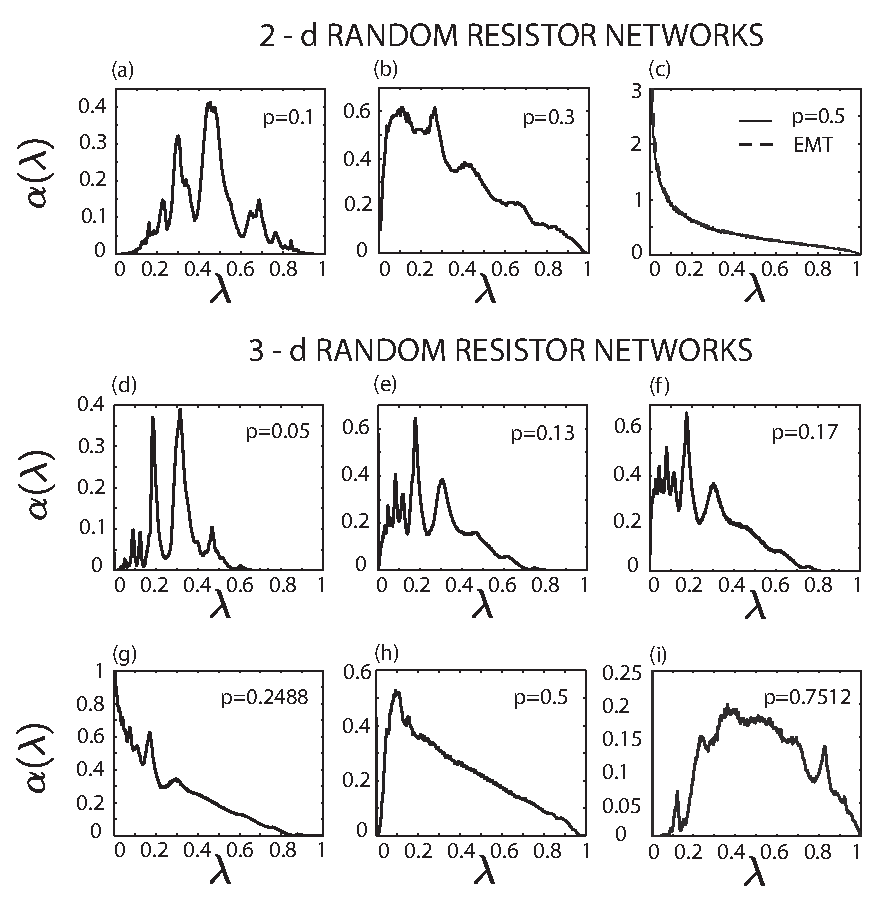
\includegraphics[width=25pc]{2-3-d_Random_Resistor_Networks.eps}
\caption{\emph{The spectral function for the 2--d and 3--d square
    random resistor networks (RRN).} In the 2--d RRN (a)--(c), as the
  volume fraction $p$ increases from left to right,
  the width of the gaps in the spectrum near $\lambda=0,1$ shrink to 0
  \emph{symmetrically} with increasing connectedness as
  $p\to p_c=1-p_c=0.5$. In (c) the effective medium theory (EMT)  
  prediction of the the spectral measure, which coincides with the
  exact duality prediction, is also displayed. In
  the 3--d RRN (d)--(i), as $p\to p_c\approx0.2488$ the width of the gap near
  $\lambda=0$ shrinks to 0, and as $p\to1-p_c\approx0.7512$ the width of the gap
  near $\lambda=1$ shrinks to 0.} 
\end{figure} \label{fig:2D-RBN}
%
%

For bond lattice systems with a finite number $n$ of 
bonds, the differential equations in \eqref{eq:Maxwells_Equations_E}
become difference equations (Kirchoff's laws)
\cite{Golden:JMP-5627}. Consequently, the operators $\mathbf{M}_j$,
$j=1,2$ are given by $N\times N$ matrices, say
\cite{Golden:JoB:337,Golden:JMP-5627} and 
the spectral measure $\alpha_{ik}(d\lambda)$ of the matrix $\mathbf{M}_2$ is
given by a sum of ``Dirac $\delta$ functions,''
%
\begin{align}\label{eq:Spectral_Function}
  \alpha_{ik}(d\lambda)=
    \left[\sum_{j=1}^N m_j \delta_{\lambda_j}(d\lambda)\right]d\lambda
      =\alpha_{ik}(\lambda)d\lambda,
\end{align}
%
where $\delta_{\lambda_j}(d\lambda)$ is the Dirac delta measure concentrated at $\lambda_j$,
$m_j=\langle\vec{e}_i^{\;T}[\vec{v}_j\vec{v}_j^{\;T}]\,\vec{e}_k\rangle$, 
$\vec{e}_k$ is a standard basis vector on the lattice, for some
$k=1,\ldots,d$, and $\lambda_j$ and $\vec{v}_j$ are the eigenvalues and
eigenvectors of $\mathbf{M}_2$, 
respectively \cite{Golden:JoB:337}. 
The associated Stieltjes transformation of the measure in
\eqref{eq:Herglotz_Funs_sed_LYRB} is  
given by the sum $G(t)=\sum_{j=1}^nm_j/(t-\lambda_j)$, and $\alpha_{ik}(\lambda)$ in equation
\eqref{eq:Spectral_Function} is called ``\emph{the spectral
  function},'' which is defined only pointwise on the set of
eigenvalues $\{\lambda_j\}$.

In Figure 1 we give a graphical
representation of the spectral measure for finite 2--$d$ and 3--$d$
RRN. It displays linearly connected peaks of histograms with bin
sizes on the order of $10^{-2}$. The apparent smoothness of the
spectral function graphs in this figure is due to the large number
($\sim10^6$) of eigenvalues and eigenvectors calculated, and ensemble
averaged. Consistent with the isotropy of the
RRN, the diagonal components $\alpha_{kk}$ are virtually identical,
positive measures of equal mass $1/d$, while the $\alpha_{ik}$, $i\neq k$, are
signed measures of zero mass, up to numerical accuracy. The $\alpha_{kk}$
do not have mass $p$, as the eigenvectors are normalized in the $l_2$
innerproduct, not that weighted by the characteristic function $\chi_2$,
like in the general theory. In Figure 1 the mass of the measures has
been scaled to the volume fraction $p$.  

We now provide an analytical proof for the existence of spectral gaps
in $\alpha_{ik}$ about the spectral endpoints $\lambda=0,1$ for arbitrary, finite
lattice systems. More specifically, for $p\ll1$, $\hat{\lambda}_0>0$ and
$\hat{\lambda}_1<1$. We focus on
$\mathbf{M}_2=\chi_2\Gamma\chi_2$ and $\alpha_{ik}$, as our results extend to 
$\mathbf{M}_1=\chi_1\Gamma\chi_1$ and $\mu_{ik}$ by symmetry. In this lattice setting, $\Gamma$  
is a real symmetric projection matrix which can be diagonalized:
$\Gamma=\mathbf{Q}\mathbf{D}\mathbf{Q}^T$, where 
$\mathbf{D}=\text{diag(1,\ldots,1,0,\ldots,0)}$ is a diagonal matrix of $L$ ones
and $N-L$ zeros,
%along the principle diagonal,
$0<L<N$ when $N\gg1$, and
$\mathbf{Q}$ is a real orthogonal matrix with columns $q_i$,
$i=1,\ldots,N$, which are the eigenvectors of $\Gamma$. More specifically,
%
\begin{align*}
  \Gamma_{i,j}=(\vec{q}_i\cdot\vec{q}_j)_L
\end{align*}
%
where 
$(\vec{q}_i\cdot\vec{q}_j)_L=\sum_{l=1}^L(\vec{q}_i)_l(\vec{q}_j)_l$, and
$(\vec{q}_i)_l$ is the $l^{\text{th}}$ component of the vector
$\vec{q}_i\in\mathbb{R}^N$. Here, we consider the non--degenerate case
$L<N$.

In the matrix case, the action of $\chi_2$ is given by that of a square
diagonal matrix of zeros and ones \cite{Golden:JoB:337}. The action
of $\chi_2$ in the matrix $\chi_2\Gamma\chi_2$ introduces a row and column
of zeros in the matrix $\Gamma$, corresponding to every diagonal entry of
$\chi_2$ with value 0. When there is only one $\sigma_2$ inclusion ($p=1/n$)
located at the $j^{\text{th}}$ bond, $\chi_2$ has all zero entries except
at the $j^{\text{th}}$ diagonal:
$\chi_2=\text{diag}(0,\cdots,0,1,0,\cdots,0)=\text{diag}(\vec{\text{v}}_j)$. Therefore, 
the only non-trivial eigenvalue is given by 
$\lambda_0=(\vec{q}_j\cdot\vec{q}_j)_L=\sum_{l=1}^L(\vec{q}_j)_l^2=1-\sum_{l=L+1}^N(\vec{q}_j)_l^2$, 
with eigenvector $\vec{\text{v}}_j$
and weight $m_0=\vec{e}_i^{\;T}\vec{\text{v}}_j\vec{\text{v}}_j^T\vec{e}_k$.
This implies that there is a gap at $\lambda=0$, $\theta_0=\sum_{l=1}^L(\vec{q}_j)_l^2>0$,
and a gap at $\lambda=1$, $\theta_1=\sum_{l=L+1}^N(\vec{q}_j)_l^2>0$. It is clear
that these bounds hold for all $\omega\in\Omega$ such that $p=1/n$ when $L<N$. We
have already mentioned that the eigenvalues of $\mathbf{M}_2$ are
restricted to the set $\{0,1\}$ when $p=1$
$(\chi_2\equiv\mathbf{I}_N)$. Therefore, there exists $0<p_0<1$ such that,
for all $p\geq p_0$, there exists a $\omega\in\Omega$ such that $\theta_0(\omega)=0$ and/or
$\theta_1(\omega)=0$. This concludes our proof.


%(\textbf{Is it worth doing the 2x2 case?})
%
% The eigenvalue problem for the case of two defect inclusions at the
% $i^{th}$ and $j^{th}$ bond is given by that of a $2\times2$ symmetric
% matrix. In this case, the non--trivial part of the matrix $\chi_2\Gamma\chi_2$
% is given by the matrix 
% % 
% \begin{align}
%   \mathbf{M}_0=
%   \left[
%     \begin{matrix}
%       (\vec{q}_i\cdot\vec{q}_i)_L&(\vec{q}_i\cdot\vec{q}_j)_L\\
%       (\vec{q}_j\cdot\vec{q}_i)_L&(\vec{q}_j\cdot\vec{q}_j)_L
%     \end{matrix}
%   \right].  
% \end{align}
% The eigenvalues are given by 
% %
% \begin{align}
% \lambda_\pm=\frac{\text{Tr}\mathbf{M}_0}{2}
% \left[1\pm\sqrt{1-\frac{4\text{Det}\mathbf{M}_0}{(\text{Tr}\mathbf{M}_0)^2}}
% \right],  
% \end{align}
% %
% where $\text{Tr}\mathbf{M}_0$ is the trace of $\mathbf{M}_0$ and
% $\text{Det}\mathbf{M}_0$ is the determinant of $\mathbf{M}_0$. By the
% symmetry of $\mathbf{M}_0$, we have $\lambda_\pm\in\mathbb{R}$. Therefore
% $\lambda_+\lambda_-=\text{Det}\mathbf{M}_0<(\text{Tr}\mathbf{M}_0/2)^2<1$, as
% $\lambda_++\lambda_-=\text{Tr}\mathbf{M}_0=(\vec{q}_i\cdot\vec{q}_i)_L+(\vec{q}_j\cdot\vec{q}_j)_L
% =2-\sum_{l=L+1}^N[(\vec{q}_i)_l^2+(\vec{q}_j)_l^2]<2$.
%

\section{Concluding Remarks}
%
We have constructed a mathematical framework which unifies the critical
theory of transport for binary composite media, in continuum and
lattice settings. We have focused on critical transitions exhibited by
the effective complex conductivity $\sigma^*=\sigma_2m(h)=\sigma_1w(z)$, as the
symmetries underlying this framework extend our results to that
regarding the effective complex resistivity
$\rho^*=\tilde{m}(h)/\sigma_1=\tilde{w}(z)/\sigma_2$. We have shown in section
\ref{sec:Measure_Equivalences} that critical transitions in transport
properties are, in general, characterized by the formation of delta
%function
components in the underlying spectral measures at the spectral
endpoints. Moreover, for percolation models, we have shown that the
onset of the critical transition (the formation of these delta
components) occurs \emph{precisely} at the percolation threshold $p_c$
and $1-p_c$.        

The mathematical transport properties of such systems, displayed in
sections \ref{eq:TACM} and \ref{sec:SF_Reps}, hold for general
two--component stationary random media in lattice and continuum settings
\cite{Golden:CMP-473}. While the critical exponent scaling relations
and the various transport properties, displayed in Lemmas
\ref{lem:nonzero_gamma1_etc}--\ref{lem:s_t}, hold for percolation
models of the composites class $\mathcal{B}_{n_\upsilon}$, $\upsilon=\phi,\ph\,$,
introduced in definition \ref{def:Bounded_diff_g}. Under the  
condition that $n_\phi,n_{\ph}\geq1$, i.e., that $m(p,0)$ and $\chi(p,0)$ in
\eqref{eq:Crit_Exponents_mh} exist for $p>p_c$, and $w(p,z(0))$ and
$\hat{\chi}(p,z(0))$ in \eqref{eq:Crit_Exponents_wh} exist for $p<p_c$,
we linked the two sets of critical exponents in
\eqref{eq:Crit_Exponents_mh} and 
\eqref{eq:Crit_Exponents_wh} showing that, for percolation models like
EMT where $n_\phi,n_{\ph}=\infty$, they are all determined by only three critical
exponents, and are determined by only two critical exponents under the 
symmetry condition of Lemma \ref{lem:s_t}. This type of critical
behavior has been studied before for the lattice
\cite{Efros:PSSB-303,Clerc:AP-191,Bergman:SSP-147}, and alternate
methods have shown that $\Delta=s+t$, $\delta=(s+t)/t$, and $\gamma=s$. These are
precisely the relations that we have shown to hold for lattice and
continuum percolation models of this class, under these
conditions. The EMT percolation model satisfies these
conditions, however, there is no apparent mathematical necessity for
these conditions to hold, in general. Although they lead to the well
known two dimensional duality relation $s=t$ for the lattice
\cite{Bergman:SSP-147,Clerc:AP-191,Efros:PSSB-303}. 


Numerical and analytical work on the
sequence of critical exponents $\tilde{\psi}(q)$ for the moments of
the current distribution in RRN, e.g.,
\cite{Stauffer-92,Blumenfeld:PRB-3524,Deuring:JSP-113}, has shown that
this sequence exhibits nonlinear dependence in $q$, or multifractal
behavior. We proved in Lemma \ref{lem:Scaling_rel_t_s_gamman} that the
exponents $\gamma_n$ have linear dependence in $n$ for all
$1\leq n\leq n_{\ph}\leq n_\phi$. This is consistent with the absence of
multifractal behavior for percolation models
of class $\mathcal{B}_{\infty}$, such as EMT. However for percolation
models with $n_{\ph},n_\phi<\infty$, multifractal behavior is not ruled out by Lemma
\ref{lem:Scaling_rel_t_s_gamman}. It is interesting, though, that the
$\tilde{\psi}(q)$ satisfy Baker's inequalities
\eqref{eq:CondBakerIneq_m} \cite{Blumenfeld:PRB-3524}.


As in EMT, our general scaling relations involving $|h|$ are
independent of the limiting path as $h\to0$. This represents an
alternative to the results of other workers
\cite{Efros:PSSB-303,Clerc:AP-191,Bergman:SSP-147} who have used
heuristic scaling forms as a starting point. For our critical theory
the starting point is equation \eqref{eq:Herglotz_Funs_sed_LYRB},
which displays \emph{exact} formulas for infinite systems
\cite{Golden:PRL-3935}. We have verified the validity of our framework
using several consistency checks including the verification that our
relations are satisfied directly by the exponents of effective medium
theory. 


% If in two-column mode, this environment will change to single-column format so that long equations can be displayed. 
% Use only when necessary.
%\begin{widetext}
%$$\mbox{put long equation here}$$
%\end{widetext}

% Figures should be put into the text as floats. 
% Use the graphics or graphicx packages (distributed with LaTeX2e).
% See the LaTeX Graphics Companion by Michel Goosens, Sebastian Rahtz, and Frank Mittelbach for examples. 
%
% Here is an example of the general form of a figure:
% Fill in the caption in the braces of the \caption{} command. 
% Put the label that you will use with \ref{} command in the braces of the \label{} command.
%
% \begin{figure}
% \includegraphics{}%
% \caption{\label{}}%
% \end{figure}

% Tables may be be put in the text as floats.
% Here is an example of the general form of a table:
% Fill in the caption in the braces of the \caption{} command. Put the label
% that you will use with \ref{} command in the braces of the \label{} command.
% Insert the column specifiers (l, r, c, d, etc.) in the empty braces of the
% \begin{tabular}{} command.
%
% \begin{table}
% \caption{\label{} }
% \begin{tabular}{}
% \end{tabular}
% \end{table}

% If you have acknowledgments, this puts in the proper section head.
\begin{acknowledgments}
We gratefully acknowledge support from the Division of Mathematical
Sciences and the Office of Polar Programs at the US National Science
Foundation through grants DMS-1009704 and ARC-0934721.
\end{acknowledgments}

% Create the reference section using BibTeX:
\bibliographystyle{plain}
\bibliography{murphy}

\end{document}
%
% ****** End of file aiptemplate.tex ******
